\documentclass[10pt]{article}
\usepackage{graphicx} % Required for inserting images
\usepackage{tabularx,lipsum,environ,amsmath,amssymb}
\usepackage{algorithm}
\usepackage{algpseudocode}
\usepackage{placeins}
\usepackage{xcolor}
\usepackage{amsthm}
\usepackage{hyperref}
\usepackage{graphicx}
\usepackage{subcaption}



\usepackage{apxproof}

\makeatletter

%\usepackage[a4paper, total={6in, 8in}]{geometry}
\usepackage[margin=1in]{geometry}


%\newtheorem{theorem}{Theorem}
%\newtheorem{lemma}{Lemma}

\newtheoremrep{theorem}{Theorem}
\newtheoremrep{lemma}{Lemma}


\newenvironment{hashtable}[1][]
  {\begin{tabular}[#1]{
     @{} 
     > {\small} r <{\normalsize~\rlap{\fbox{\strut~~}}$~~\rightarrow$~}
     @{} l @{}}}
  {\end{tabular}}


\newcommand{\lca}{\texttt{lca}}

\newcommand{\problemtitle}[1]{\gdef\@problemtitle{#1}}% Store problem title
\newcommand{\probleminput}[1]{\gdef\@probleminput{#1}}% Store problem input
\newcommand{\problemquestion}[1]{\gdef\@problemquestion{#1}}% Store problem question
\NewEnviron{problem}{
  \problemtitle{}\probleminput{}\problemquestion{}% Default input is empty
  \BODY% Parse input
  \par\addvspace{.5\baselineskip}
  \noindent
  \begin{tabularx}{\textwidth}{@{\hspace{\parindent}} l X c}
    \multicolumn{2}{@{\hspace{\parindent}}l}{\@problemtitle} \\% Title
    \textbf{Input:} & \@probleminput \\% Input
    \textbf{Problem:} & \@problemquestion% Question
  \end{tabularx}
  \par\addvspace{.5\baselineskip}
}
\makeatother

\newcommand{\ml}[1]{\begingroup\color{blue}#1\endgroup}
\newcommand{\rk}[1]{\begingroup\color{red}#1\endgroup}

\title{Tractable Phylogenomics Reconciliation}
\author{Reza Kalhor, Manuel Lafond, Celine Scornavacca}
\date{}

\begin{document}

\maketitle


\begin{abstract}
    Abstract here, note that title page does not count.
    Also find a better paper title.
\end{abstract}

\newpage




\section{Introduction}

%\rk{The evolutionary paths of gene families often deviate from the species' history due to macro-evolutionary events beyond simple speciation. This divergence can arise from various factors, such as gene duplication, gene loss, horizontal gene transfer, or incomplete lineage sorting \cite{maddison1997gene}. To reveal these macro-evolutionary events, reconciliation methods are used to align gene trees with the species tree by analyzing the discrepancies between their topologies \cite{goodman1979fitting, page1994maps}.} 

Gene duplication is a fundamental mechanism for the development of novel functions and species adaptation~\cite{ohno1970evolution}. 
Inferring past duplication events is therefore essential in understanding evolution, with applications ranging from 
reconstructing ancestral genomes~\cite{duchemin2017decostar}, inferring functionally similar genes~\cite{ullah2015integrating,lafond2018accurate,hellmuth2015phylogenomics}, \ml{[and XYX]}.
\emph{Reconciliation} is commonly used to infer duplications, among other events, by explaining the discrepancies between a gene tree and a species tree~\cite{goodman1979fitting}.
There are now several tools for reconciliation~\cite{doyon2010efficient,jacox2016eccetera,durand2006hybrid,bansal2018ranger}, most of them tailored for the comparison of an individual gene tree against a species tree.  This assumes that gene families can be reconciled independently, although it is well-known that ancestral macro-evolutionary events can be segmental and affect multiple genes.  A striking example includes \emph{whole genome duplication} (WGD), which copies the entire genome and doubles all of the gene content [REFS] \ml{[maybe discuss importance of WGD, see ~\cite{gorecki2024unifying} for refs]}.  Since reconciling gene families separately may miss such events, \emph{phylogenomics reconciliation} incorporates multiple gene families and trees simultaneously for the prediction of ancestral events.

% \rk{Examining these macro-evolutionary events helps us gain a clearer understanding of evolutionary mechanisms and improves our ability to reconstruct ancestral genomes \cite{dondi2017approximating, lafond2016link, lafond2018accurate, ullah2015integrating}. Moreover, since gene families are interconnected in their evolution, a robust approach would be to reconcile multiple gene trees simultaneously while specifically accounting for segmental duplications—events that impact entire chromosome segments rather than individual genes \cite{duchemin2017decostar}.} (several models infer duplications and losses, most assume that gene histories are independent, even though segmental events are know to occur, lca is the de facto standard, etc) 
Guigo et al.~\cite{guigo1996reconstruction} were among the first to extend reconciliation to multiple gene trees.  They developed heuristics for this task, until Page and Cotton~\cite{page1994maps} formalized it into the \emph{Episodes Clustering} (EC) problem, which asks to map the duplication events into a minimum number of species.  This was later extended to a variant called \emph{Minimum Episodes} (ME)~\cite{bansal2008multiple}, where the number of duplication rounds within each species is also counted \ml{[todo: backcheck if this description is accurate]}.
There are very efficient algorithms for these problems~\cite{luo2009linear,mettanant2008linear,paszek2017efficient} and related variants (see e.g.~\cite{gorecki2024unifying}, and~\cite{paszek2017efficient} for a survey), but these models have inherent drawbacks.  First, the speciation events predicted by the \emph{lca-mapping}, which maps genes to their latest possible species, usually cannot be contested.  This in turn fixes the set of duplications \emph{a priori}, before searching for segmental events, which significantly reduces the space of considered reconciliations.  Indeed, the range of possible species of ancestral genes is limited by the lca-mapping speciations, even though several works argue that alternate scenarios should be explored~\cite{doyon2011efficient,arvestad2003bayesian}.  Second, these models do not consider gene losses, even though they are informative as they often eliminate redundancy after large-scale duplications.  

Recently, Delabre et al. \cite{delabre2018reconstructing,anselmetti2022reconciliation} introduced a multi-gene reconciliation model that does handle losses.  They aim to reconstruct the evolution of syntenic blocks, which can be used to infer segmental duplication events.  However, the scale of such events is limited by the size of detectable syntenies among dozens of species, which is usually small.  The model also requires all the gene families within a block to evolve in compatible gene trees, making the approach not always usable in practice.

%\rk{In this direction, three primary models have been explored: Episode Clustering (EC), Minimum Episodes (ME)~\cite{bansal2008multiple, guigo1996reconstruction}, and Multiple Gene Duplication (MGD)~\cite{fellows1998multiple}. Both the EC and MGD formulations focus on grouping duplications by minimizing the number of locations in the species tree where at least one duplication occurred. The MGD problem introduces an additional constraint: a cluster cannot contain two gene duplications from the same gene tree. Among these, the ME problem is considered more biologically relevant because it aims to minimize the actual number of segmental duplications. Most exact solutions proposed for the ME problem \cite{luo2009linear, paszek2017efficient} focus on a constrained version, where the possible mappings of a gene tree node are limited to specific intervals \cite{bansal2008multiple}. Additionally, Delabre et al. \cite{delabre2018reconstructing} explored the reconstruction of syntenic block evolution. Their model allows for segmental duplications but is more restrictive, requiring that every gene family within a block evolves along the same tree.}

In this work, we focus on a reconciliation approach that avoid the aforementioned drawbacks: it infers segmental duplications in a model that is \emph{synteny-free}, that \emph{considers losses}, and that is \emph{not restricted by the lca-mapping}.
The model was introduced in~\cite{dondi2019reconciling}
and, unlike previous multi-gene approaches, allows all time-consistent gene-species maps and speciation events to be relabeled to duplications --- such remappings imply gene losses, which naturally limit how far a gene can be remapped with respect to the lca-mapping.
%Although several models have been introduced to find segmental duplications, their power over the traditional lca-mapping is unclear.   To our knowledge, it has not been established whether there are situations where the lca-mapping cannot find enough evolutionary signals to recover segmental events accurately.  In this work, we focus on comparing the lca-mapping with the reconciliation model introduced in [REF] \cite{dondi2019reconciling}, which considers segmental duplications and single losses. 
Finding a most parsimonious reconciliation under this model was shown to be NP-hard, but a $O(\lceil \delta/\lambda \rceil^d \cdot n)$ time algorithm is known, where $\delta$ is the cost of a segmental duplication, $\lambda$ is the cost of a single loss, and $d$ is the number of segmental duplications in an optimal scenario. 



Unfortunately, the implementation of this algorithm can only handle small datasets - it could not terminate on modest simulated instances with around 30 species and 100 gene trees.  Moreover, the base $\lceil \delta/\lambda \rceil$ of the exponential complexity only allows small duplication/loss ratios, which has the same undesired effect of limiting the range of possible species of ancestral genes as previous work.  
Due to these limitations, the potential of the novel model has not been fully explored.  Since practical exact algorithms appear difficult to achieve, we turn to heuristics to explore this question.  We introduce an approach inspired by simulated annealing that starts with a given initial reconciliation, then explores the solution space by performing gene remapping moves until convergence.  
%This can be used in a greedy manner in a hill-climbing strategy by always choosing the optimal move until exhaustion, or stochastically by assigning a probability to each move based on their change in reconciliation cost.  
The supported moves include remapping a single gene to a higher or lower species, or remapping a whole segmental duplication in a single move.

Even with this simple strategy, the gargantuan size of the solution space comes with algorithmic challenges.  In datasets of moderate size, there can be hundreds of thousands of possible moves, which need to be re-evaluated at each iteration.  Minimizing the computation time per iteration is therefore crucial, leading to the combinatorial problem of evaluating the change in cost of each move. 
We propose a dynamic programming algorithm that computes the cost impact of each such move in O(1) amortized time, allowing phylogenmics reconciliation that scales to thousands of gene trees.  


We implemented our approach and performed extensive experiments to assess the potential in recovering large-scale segmental duplications.  To our knowledge, the added value of phylogenomics reconciliation against the traditional lca-mapping has not been established clearly in the literature.  It may well be that the latter performs just fine and that sophisticated reconciliation models are not needed.  Our experiments say otherwise though.  
Indeed, in the presence of WGD, we show on SimPhy simulations that the standard lca-mapping may map ancestral genes incorrectly, and even indicate incorrect WGD locations.  This is mostly due to the fractionation and complex loss patterns that follows WGD, to which our approach exhibits more robustness.

This trend is confirmed on real data.  We analyze three sets of species known to have undergone one or more WGD.  \ml{buff this part later}








\section{Methods}

We first formalize our reconciliation model, then discuss our efficient exploration of the solution space.
We use the standard notions of trees, forests, height, and distance, and refer the reader to the appendix for complete definitions.
The root of a tree $T$ is denoted $r(T)$;  its set of leaves is $L(T)$ and its height is $h(T)$.  The \emph{distance} between two nodes $u, v$ of $T$ is $dist_T(u, v)$. 
The set of trees in a forest $F$ is denoted $t(F)$.  The leaves of $F$ are $L(F) = \bigcup_{T \in t(F)} L(T)$, and the \emph{height} of $F$ is $h(F) = \max_{T \in t(F)} h(T)$.
The subgraph of $F$ induced by $X$ is denoted $F[X]$.
For $u, v \in V(F)$ in the same tree, we write $u \preceq_F v$ if $u$ is a descendant of $v$, and $u \prec_F v$ when $u \neq v$.  Two nodes $u, v$ of $F$ are \emph{incomparable} if neither is an ancestor of the other.
If $X \subseteq L(F)$ is a set of leaves that all belong to the same tree of $t(F)$, we write $\lca_F(X)$ for the lowest common ancestor of $X$.   We may drop the subscript $F$ in the notation if unambiguous.
%Note that a tree is a special case of a forest, so all the above notation also applies to trees.











\paragraph{Reconciliations.}
A \emph{gene tree} is a tree in which the leaves contain extant genes, and 
a \emph{gene forest} is a forest $G$ of gene trees.  A \emph{species tree} is a tree $S$ in which $L(S)$ is a set of extant species. 
A \emph{leaf species map} is a function $\sigma : L(G) \rightarrow L(S)$ that assigns each extant gene to its extant species.

Given a gene forest $G$, a species tree $S$, and a leaf species map $\sigma$, a \emph{reconciliation} is a map $m : V(G) \rightarrow V(S)$ that assigns each gene forest node to a species node.
Moreover, $m$ must satisfy the following conditions:\\
\emph{1. preserve leaf maps}: for each $u \in L(G)$, $m(u)=\sigma(u)$;\\
\emph{2: time consistency}: for each non-root node $u \in V(G)$ with parent $p_u$, we have $m(u) \preceq_S m(p_u)$.

The \emph{lca-mapping} between $G$ and $S$ is the unique reconciliation $\mu$ that assigns each node to to the lowest possible species according to time-consistency (see Figure~\ref{fig:fig1} top row).  That is, for each internal node $u$ of $G$, 
$\mu(u) = \lca_S( \{ \sigma(w) : w \in L(G) \mbox{ and } w \preceq u \} )$.  \ml{todo: check if I reconciled correctly in fig}


\begin{figure}[htb]
    \centering
    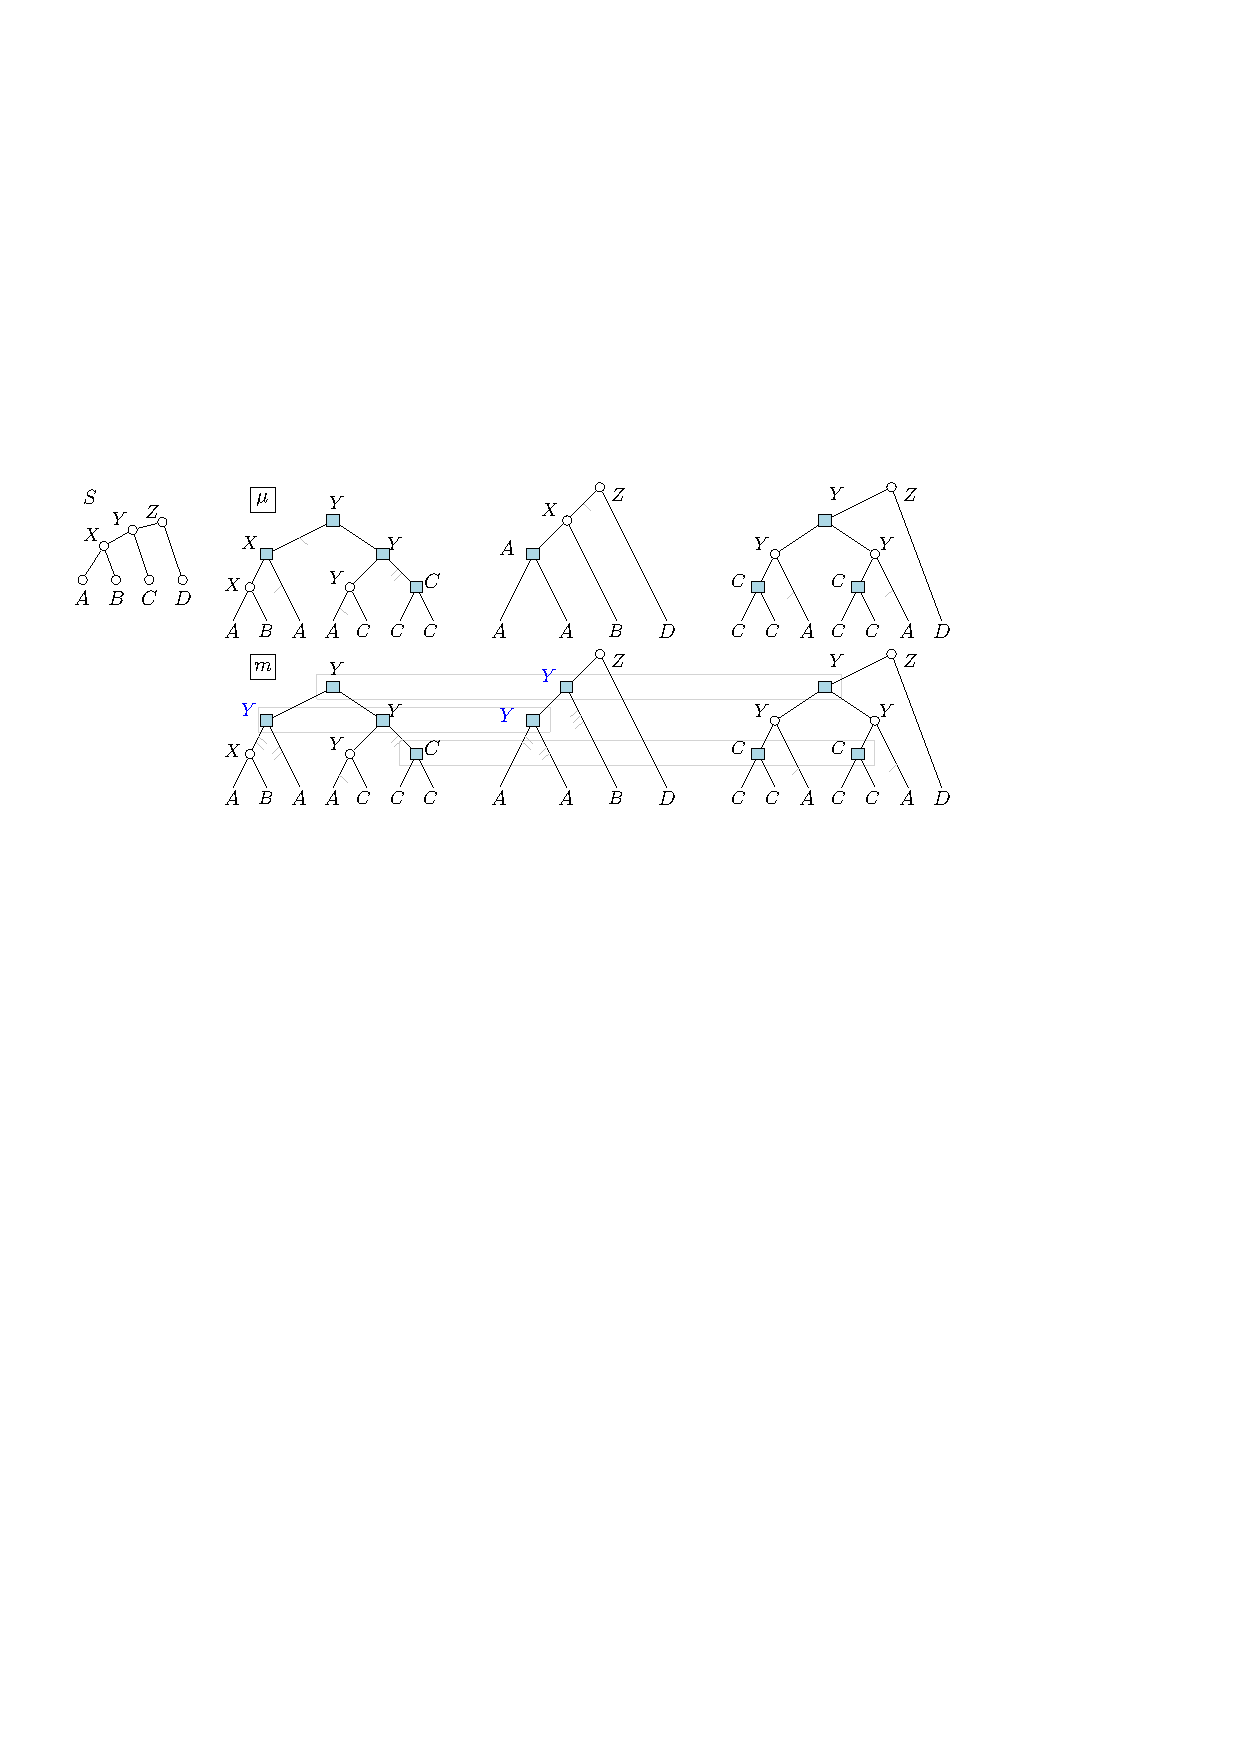
\includegraphics[width=0.8\linewidth]{figs_theory/fig1.pdf}
    \caption{Two possible reconciliations for a species tree $S$ and a forest of three gene trees.  Each leaf is labeled by $\sigma$, the species that contains it, and internal nodes are labeled according to $\mu$ (top) or $m$ (bottom).
    Blue squares are $Dup$ nodes, white circles are $Spec$ nodes, and light gray edges are losses.
    The reconciliation $m$ can be explained with three segmental duplications (gray rectangles), whereas $\mu$ needs five.
    }
    \label{fig:fig1}
\end{figure}


\paragraph{Speciation, duplication, and loss.}
We use an established framework~\cite{gorecki2006dls,zhang1997mirkin} to infer whether each internal node of $G$ underwent a speciation ($Spec$) or duplication ($Dup$) event under a reconciliation $m$.  In essence, we infer a speciation at $u$ if its children branched into two separate species.
The \emph{event labeling under $m$} is that function $ev_m : V(G) \setminus L(G) \rightarrow \{Spec, Dup\}$ that, for each $u \in V(G)$ with children $u_1, u_2$, puts:
\begin{align*}
    ev_m(u) = \begin{cases}
        Spec & \mbox{if $m(u_1)$ has children $x_1, x_2$ such that } \mbox{$u_1 \preceq_S x_1$ and $u_2 \preceq_S x_2$}\\
        Dup &\mbox{otherwise.}
    \end{cases}
\end{align*}
A node $u \in V(G)$ with $m(u) = s$ and $ev_m(u) = Dup$ is called an \emph{$s$-duplication} (with respect to $m$).
As an example, in middle gene tree of Figure~\ref{fig:fig1}, the node mapped to $X$ according to $\mu$ is a $Spec$ (top), but the same node mapped to $Y$ according to $m$ is a $Dup$ (bottom).

Gene losses are counted on the branches of $G$ by listing the species that should be present but are not.  For an edge $uv \in E(G)$, the number of losses on $uv$ is $dist_S(m(u), m(v)) - 1$ if $ev_m(u) = Spec$, and $dist_S(m(u), m(v))$ if $ev_m(u) = Dup$. 
The total number of losses under $m$ is
$l_m = \sum_{uv \in E(G)} l_m(uv)$.






\paragraph{Segmental duplications.}
For a species $s \in V(S)$, the \emph{duplication forest} of $s$ (under $m$), denoted $F_m(s)$, is the subgraph of $G$ induced by $s$-duplications.  Formally: 
$F_m(s) = G[ \{v \in V(G) : m(v) = s, ev_m(v) = Dup\}]$.
A \emph{segmental duplication} is a single duplication event that contains multiple genes.  Such genes must coexist in the same species and must be incomparable in $G$ and $F_m(s)$, and so it is not hard to see that 
the smallest possible number of segmental duplications in species $s$ is the height of $F_m(s)$, which we recall is $h(F_m(s))$.  The total number of segmental duplications in $m$ is thus 
$d_m = \sum_{s \in V(S)} h(F_m(s))$.
For example in Figure~\ref{fig:fig1}, $d_{\mu} = 5$ (two duplications in $Y$, one in $X, A, C$), whereas $d_m = 3$ (two duplications in $Y$, one in $C$).
We can finally state our problem formulation.

\medskip

\noindent 
The \textsc{Most Parsimonious Segmental Reconciliation} problem

\noindent 
\textbf{Input:} a gene forest $G$, a species tree $S$, a leaf species map $\sigma$, and a duplication cost $\delta$ and loss cost $\lambda$.

\noindent 
\textbf{Goal:} find a reconciliation $m$ between $G$ and $S$ that minimizes the cost 
$\delta \cdot d_m + \lambda \cdot l_m$.








\subsection*{Efficient exploration of the solution space}

To solve the above problem, we propose the following strategy to explore the space of reconciliations:  

\medskip

\noindent
1) start with an initial reconciliation $m$ (typically the lca-mapping $\mu$); \\
2) for each gene node $u \in V(G)$, and for each species $s$, compute the change in cost if we remap $u$ to $s$; \\
3) choose one of the moves from the previous step according to some criteria, and apply it; \\
4) repeat step 2 until no more moves need to be considered.

\medskip

The types of ``remapping moves'' that we consider at step 2 follows, and then we discuss step 3.

\begin{figure}[b]
    \centering
    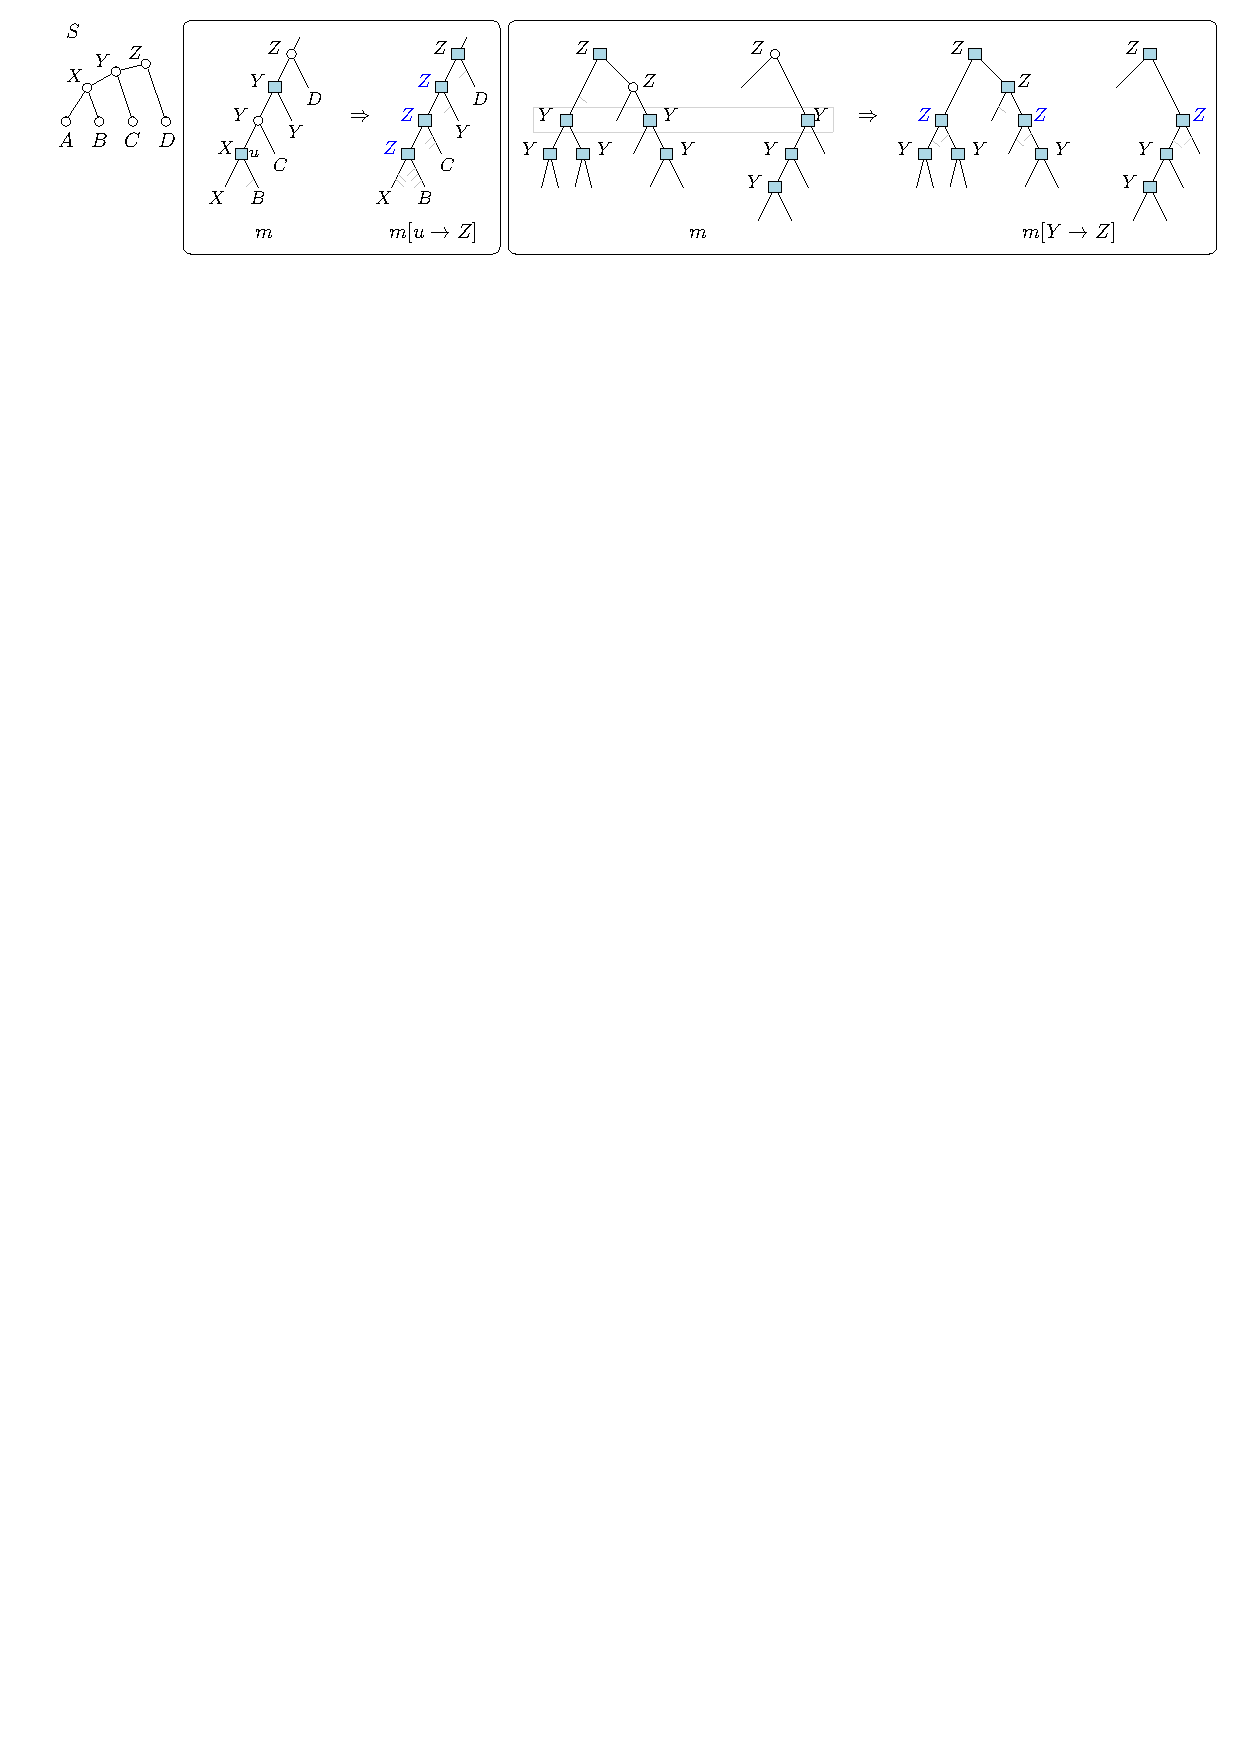
\includegraphics[width=1\linewidth]{figs_theory/upmoves.pdf}
    \caption{An illustration of up-moves and bulk up-moves.  Left: the species tree $S$.  Middle: a portion of a gene tree undergoing an up-move that remaps $u$ from $X$ to $Z$.  To satisfy time-consistency, the parent and grand-parent of $u$ must also be remapped to $Z$, which creates a chain of duplications in $Z$ and additional losses.  Right: a bulk up-move that takes the earliest segmental duplication in $Y$ spanning two gene trees, which consists of the roots of the trees in $F_m(Y)$, and remaps them to the species $Z$.}
    \label{fig:up-moves}
\end{figure}

\medskip 

\noindent 
\textbf{Up-moves.}
Let $u \in V(G)$ and $s \succ m(u)$.  Remapping $u$ to $s$ may create time-inconsistencies with its parent $p_u$, for instance if we remap $u$ to a species that pre-existed $m(p_u)$.  Our moves can thus also remap ancestors to preserve time-consistency.  See Figure~\ref{fig:up-moves} left box for an example, where remapping $u$ to $Z$ enforces remapping all the ancestors in $Y$.
The \emph{up-remapping of $u$ to $s$} is another mapping $m[u \rightarrow s]$ in which: \\
(1) $m[u \rightarrow s](w) = s$ for every ancestor $w$ of $u$ such that $m(w) \prec s$ (including $u$); \\
(2) $m[u \rightarrow s](w) = m(w)$ for every other node of $G$.

We note that considering up-moves that can remap ancestors allows a much more efficient exploration than restricting to moves that cannot.  If only the latter were allowed, we may be forced into a valley of high-cost reconciliations before finding an improvement (this occurs in Figure~\ref{fig:up-moves}, see appendix for details).



\medskip 

\noindent
\textbf{Bulk up-moves.}  We may need to remap several genes upwards to save a segmental duplication.  One way is to take the genes in the same segmental duplication in some species $s$, and move that duplication to an ancestor of $s$.
For $s \in V(S)$ and $t \succ s$, the \emph{bulk up-remapping from $s$ to $t$}
is another mapping $m[s \rightarrow t]$ in which, for every root $u$ of the forest $F_m(s)$, we apply the up-move that remaps $u$ to $t$ (in any order).  



Such bulk up-moves always reduce the height of $F_m(s)$, although they can increase
the duplication height of other species.  
This is illustrated in Figure~\ref{fig:up-moves}, where the roots of the $Y$ duplication forest are all remapped to $Z$, thereby reducing the number of segmental duplications in $Y$, but increasing those in $Z$ in this case.  
%Also note that such a move is guaranteed to increase the number of losses.  Therefore, they can only be advantageous if they reduce the height of $F_m(s)$ without increasing another height.  
%A bulk up-remapping from $s$ to $t$ will be called \emph{admissible} if $d_{m[s \rightarrow t]} < d_m$. 






\medskip 

\noindent 
\textbf{Down-moves.}
A down-move remaps $u \in V(G)$ to a species $s$ below $m(u)$.  Since $\mu(u)$ is the lowest possible, such an $s$ must satisfy $\mu(s) \preceq s \prec m(u)$, and we may need to remap descendants of $u$ to $s$ to avoid time-inconsistencies.
The \emph{down-remapping of $u$ to $s$} is another mapping $m[u \rightarrow s]$ in which: \\
(1) $m[u \rightarrow s](w) = s$ for every descendant $w$ of $u$ such that $m(w) \succ s$ (including $u$);\\
(2) $m[u \rightarrow s](w) = m(w)$ for every other node of $G$.
    


Notice that the notation $m[u \rightarrow s]$ does not distinguish between up-moves and down-moves, that distinction can be deduced from $s$.
Also note that unlike up-moves, applying a down-move to $u$ may make it change from a $Dup$ node to a $Spec$, and even its parent $p_u$ can become a $Spec$.


\medskip 

\noindent
\textbf{Bulk down-moves.} As for up-moves, several genes may be remapped ``downwards'' at once to save a duplication (or more).  Here, we take the deepest segmental duplication in $s$, and move it to a lower species.

For $s \in V(S)$ and $t \prec s$, the \emph{bulk remapping from $s$ to $t$} is another mapping $m[s \rightarrow t]$ that takes each deepest leaf $u$ of $F_m(s)$, that is, every $u$ of maximum depth $h(F_m(s))$, and applies the down-remapping of $u$ to $t$.  If such a down-move is not possible because $\mu(u) \preceq t \prec s$ does not hold, then $m[s \rightarrow t]$ is \emph{invalid}.  

\paragraph{Strategies and bottlenecks.}
We consider two strategies to implement Step 3) abvoe, which chooses a move.  
The \emph{greedy} strategy simply chooses the move that yields the lowest reconciliation cost.  The \emph{stochastic} strategy assigns each possible reconciliation $m'$ a weight $w_{m'} = e^{r / (kT)}$, where $k$ is the Boltzmann constant and $T$ is a user-specified \emph{temperature} parameter.  It then normalizes the weights to obtain a probability distribution and then chooses randomly.  We stop when convergence is reached or when a specified maximum number of iterations is achieved.


The main bottleneck of our exploration procedure is Step 2), the computation of cost changes of each move.  Its complexity controls the number of iterations we can perform in reasonable time.  
A naive implementation takes time $O(|V(G)|^2 h(S))$ to compute every entry, per iteration (see appendix).   
Since we need to scale to gene forests with thousands of trees and tens of thousands of nodes, a quadratic dependency on $|V(G)|$ is not acceptable.  In the following, we aim for an amortized time of $O(1)$ per entry.

\subsubsection*{Computing the change in cost of up-moves}

We briefly a dynamic programming strategy to compute up-moves quickly.    
Consider an up-move $m[u \rightarrow s]$ that remaps $u$ to $s \succ m(u)$. 
For any $t \in V(S)$, 
we denote $\Delta(u, s, t) = h(F_{m[u \rightarrow s]}(t)) - h(F_m(t))$, which is the change in duplication height in species $t$ after remapping $u$ to $s$. 
Then denote
$\Delta(u, s) = \sum_{t \in V(S)} \Delta(u, s, t)$, the \emph{total} change in duplication heights after remapping $u$ to $s$. 

If we calculate those in pre-order on $G$ (i.e, parents are handled before children), then we can re-use the information from the parents and only require a constant number of entries.  

\begin{lemma}\label{lem:deltasum}
    Let $u \in V(G)$ and let $s \in V(S)$ be an ancestor of $m(u)$.
    If $u$ is a root, or if $u$ has parent $p_u$ satisfying $s \prec m(p_u)$, then $\Delta(u, s) = \Delta(u, s, s) + \Delta(u, s, m(u))$.
    Otherwise, $u$ has a parent $p_u$ satisfying $s \succeq m(p_u)$, in which case
    %\begin{align*}
    $\Delta(u, s) = \Delta(p_u, s) - \Delta(p_u, s, s) - \Delta(p_u, s, m(u)) 
    + \Delta(u, s, s) + \Delta(u, s, m(u)).$
    %\end{align*}
\end{lemma}

\begin{proofsketch}
	If $u$ is a root, it suffices to notice that only $u$ gets remapped, and only the heights in $m(u)$ and $s$ can change.    If $s \prec m(p_u)$, again only the $u$ gets remapped, and the type of $p_u$ ($Spec$ or $Dup$) does not get affected, and the same argument applies.  In the last case, the remapping only affects duplications in $s, m(u)$, or $t$ with $m(u) \prec t \prec s$.  For those, the set of $t$-duplications that get removed is the same whether we remap $u$ to $s$ or $p_u$ to $s$, because such a duplication must be a strict ancestor of $u$.  Hence the difference in duplication heights for those $t$'s is already counted in $\Delta(p_u, s)$.  It is possible to have differences in $s$ or $m(u)$ though, so we take $\Delta(p_u, s)$, remove $\Delta(p_u, s, s)$ and $\Delta(p_u, s, m(u))$ which could be different, and replace them with $\Delta(u, s, s)$ and $\Delta(u, s, m(u))$.
\end{proofsketch}



    As a consequence of Lemma~\ref{lem:deltasum}, using a top-down approach, one can obtain $\Delta(u, s)$ by reusing $\Delta(p_u, s)$ and computing only four additional values, at most.
    This is far from being over though, as these are not trivial to obtain in $O(1)$ time each.  Computing these values require information from other trees in the forest, which in turn require maintaining auxiliary data structures efficiently.  In a similar fashion, we can also compute the change in number of losses after remapping $u$ to $s$, which we denote as $\Lambda(u, s)$.  This is easier if $\Lambda(p_u, s)$ is known, since then we only need to look around $u$ locally to infer additional losses.  
    Those techniques are all detailed in the appendix, as well as the analogous bottom-up algorithms to compute the change in costs of down-moves.  The summary of our technical results is the following (by amortized time, we mean that each entry takes time $O(1)$ to compute on average).

\begin{theorem}\label{thm:mainthm}
Given a gene forest $G$, a species tree $S$, and a reconciliation $m$, the values of $\Delta(u, s)$ and $\Lambda(u, s)$ for up-moves and down moves can be computed in amortized time $O(1)$ per entry.
\end{theorem}





\paragraph{Estimating bulk up-moves and bulk down-moves}
It is quite challenging to efficiently compute the exact change in cost of every possible bulk move.  Instead, we focus on moves that are guaranteed to be advantageous, and use upper bounds on their change in cost.
Recall that in a bulk up-move $m[s \rightarrow t]$, we remap all the roots of the $s$-duplication subtrees of $F_m(s)$ to $t$.  With the data structures necessatry to achieve Theorem~\ref{thm:mainthm}, these are easy to obtain.  The move reduces the height in $s$-duplications by $1$, but might increase the height in other species.
If the latter happens, no reduction in segmental duplications occurs and because up-moves create losses, the move will not be advantageous and we ignore it.  We can detect this, and only add up-moves that reduce the number of segmental duplications in the list of candidates by $1$.  The number of losses of a bulk up-move can be estimated as the sum of losses created by moving each gene individually, stored when computing the $\Lambda$ values.
For bulk down-moves, we use a similar idea --- when considering a move $m[s \rightarrow t]$ with $t \prec s$, we take all the deepest nodes in the forest $F_m(s)$, and try to remap those to $t$.  If this is invalid, or if such a remapping would increase the number of segmentnal duplications, we ignore the move.  We can show that the list of candidate bulk moves can be built in total time $O(|V(G)| h(S))$, which does not add complexity to Theorem~\ref{thm:mainthm}.



\section{Results}

We evaluated our algorithms on (i) simulated trees with known WGD locations on the species tree; and (ii) three real datasets with well-documented WGDs. 
We compare our predicted segmental duplications against the lca-mapping, starting with the simulations.
\ml{[Should we have a name for the software?]}


\paragraph{Simulation of species and gene trees.}  We used SimPhy \cite{mallo2016simphy}, a comprehensive simulator for the evolution of multiple gene families in a species tree. 
Since SimPhy cannot replicate the effects of a WGD, we borrow ideas from \cite{gorecki2024unifying} by planting WGDs.  This is achieved by simulating a species tree, copying one of its subtrees, and letting Simphy evolve on the modified species tree.
One key aspect to consider after a WGD is \emph{fractionation}: since duplicated genes become redundant, there is often a gradual loss of one copy to restore genomic balance and reduce metabolic costs~\cite{lynch2000evolutionary, birchler2007gene, rabier2014detecting} \ml{[are Celine's refs here?]}. 
We enforced fractionation in a post-processing step: in each gene tree $G$, a leaf $v$ was deleted with probability $(n - 1)/n$, where $n$ is the number of leaves of $G$ in the same species as $v$.
We used several distributions of duplication and loss rates in SimPhy: fixed rates (F) between 1e-6 and 1e-18, uniformly distributed (U) per node in the range $[$1e-12,1e-6$]$; lognormally distributed (LN) with location in $[$-25,-15$]$ and scales in $\{0.1,0.3,1\}$.
Incomplete Lineage Sorting (ILS) and gene transfers were not activated.
For each set of parameters, we generated 100 simulations (called runs), each with 100 gene trees and a species tree having a random number of leaves between 30 and 80.
To assess the robustness of our reconciliations, we also experimented on a modified dataset in which we applied, on each gene tree, between 1 and 15 nearest neighbor interchanges (NNI), which can replicate the effect of reconstruction errors and ILS.



\paragraph{Evaluation metrics.}  We first  compared our inferred gene-species maps against the lca-mapping, using the (known) simulated maps as our ground truth.  
We used the \emph{path distance metric} for this purpose \cite{moulton1999retractions}.
Given the true SimPhy map $s$ and an inferred map $m$, the path distance is  
$pathdist(s, m) = \sum_{v \in V(G)} dist_S(s(v), m(v))$, i.e., the sum of distances between the true and inferred species for each gene.  Our values of path distances were similar to the lca-mapping. A more appreciable difference was seen when quantifying the percentage of improvement over lca.  Given the true SimPhy maps $s_1, \ldots, s_{100}$ on the 100 gene trees of pme simulation, our inferred maps $m_1, \ldots, m_{100}$, and  the lca-maps $\mu_1, \ldots, \mu_{100}$ we computed:
$\text{Improvement (\%)} = \left(1 - \frac{\sum_{i=1}^{100} pathdist(s_i, m_i)}{\sum_{i=1}^{100} pathdist(s_i, \mu_i)}\right) \times 100$. 
Note that the denominator was never $0$ in our experiments.
We also assessed the improvements of our approach in recovering WGD events. 
We posited that a species is considered to have undergone a WGD if it exhibits a duplication in more than 80\% of the gene trees.  Comparing the inferred WGDs from our maps and the lca-maps against the known planted WGDs allowed us to calculate the number of true positives/negatives and false positives/negatives, from which we obtained precision and recall values.




\paragraph*{Simulations results.}  Figure~\ref{fig:imp_1wgd} shows the improvement percentage for several duplication costs $\delta \in \{2, 5, 30, 100\}$ (the loss cost $\lambda$ is $1$).  Note that $\delta \leq 1$ yields the lca-mapping~\cite{dondi2019reconciling}. Smaller $\delta$'s make conservative moves, since remapping a gene much higher than its lca creates too many losses for its worth.  Thus for $\delta = 2$, the improvements are smaller but present.  At the other extreme, for $\delta = 100$ (equal to the number of gene trees), genes are remapped aggressively.   On smaller D\&L rates, most duplications are due to the planted WGD, in which case these remaps can recover it.  Under higher rates, most duplications are punctual, making them difficult to distinguish them from WGDs --- with $d = 100$ we tend to cluster those duplications in one species, leading to incorrect maps.  

\ml{[ML: I'm ok with this plot.  Maybe it's possible to save space by moving the plot to the right, and adding 2 boxes on top of each other on the right.  For instance, maybe add amplitudes (lca vs d100) on the right, and explain in the text.  Or maybe precision and recall?  In nay case, we need to use that space.]}


\begin{figure}[hbt!]
    \centering
    % First subfigure on the left (full height)
    \begin{subfigure}[t]{0.58\textwidth}
        \centering
        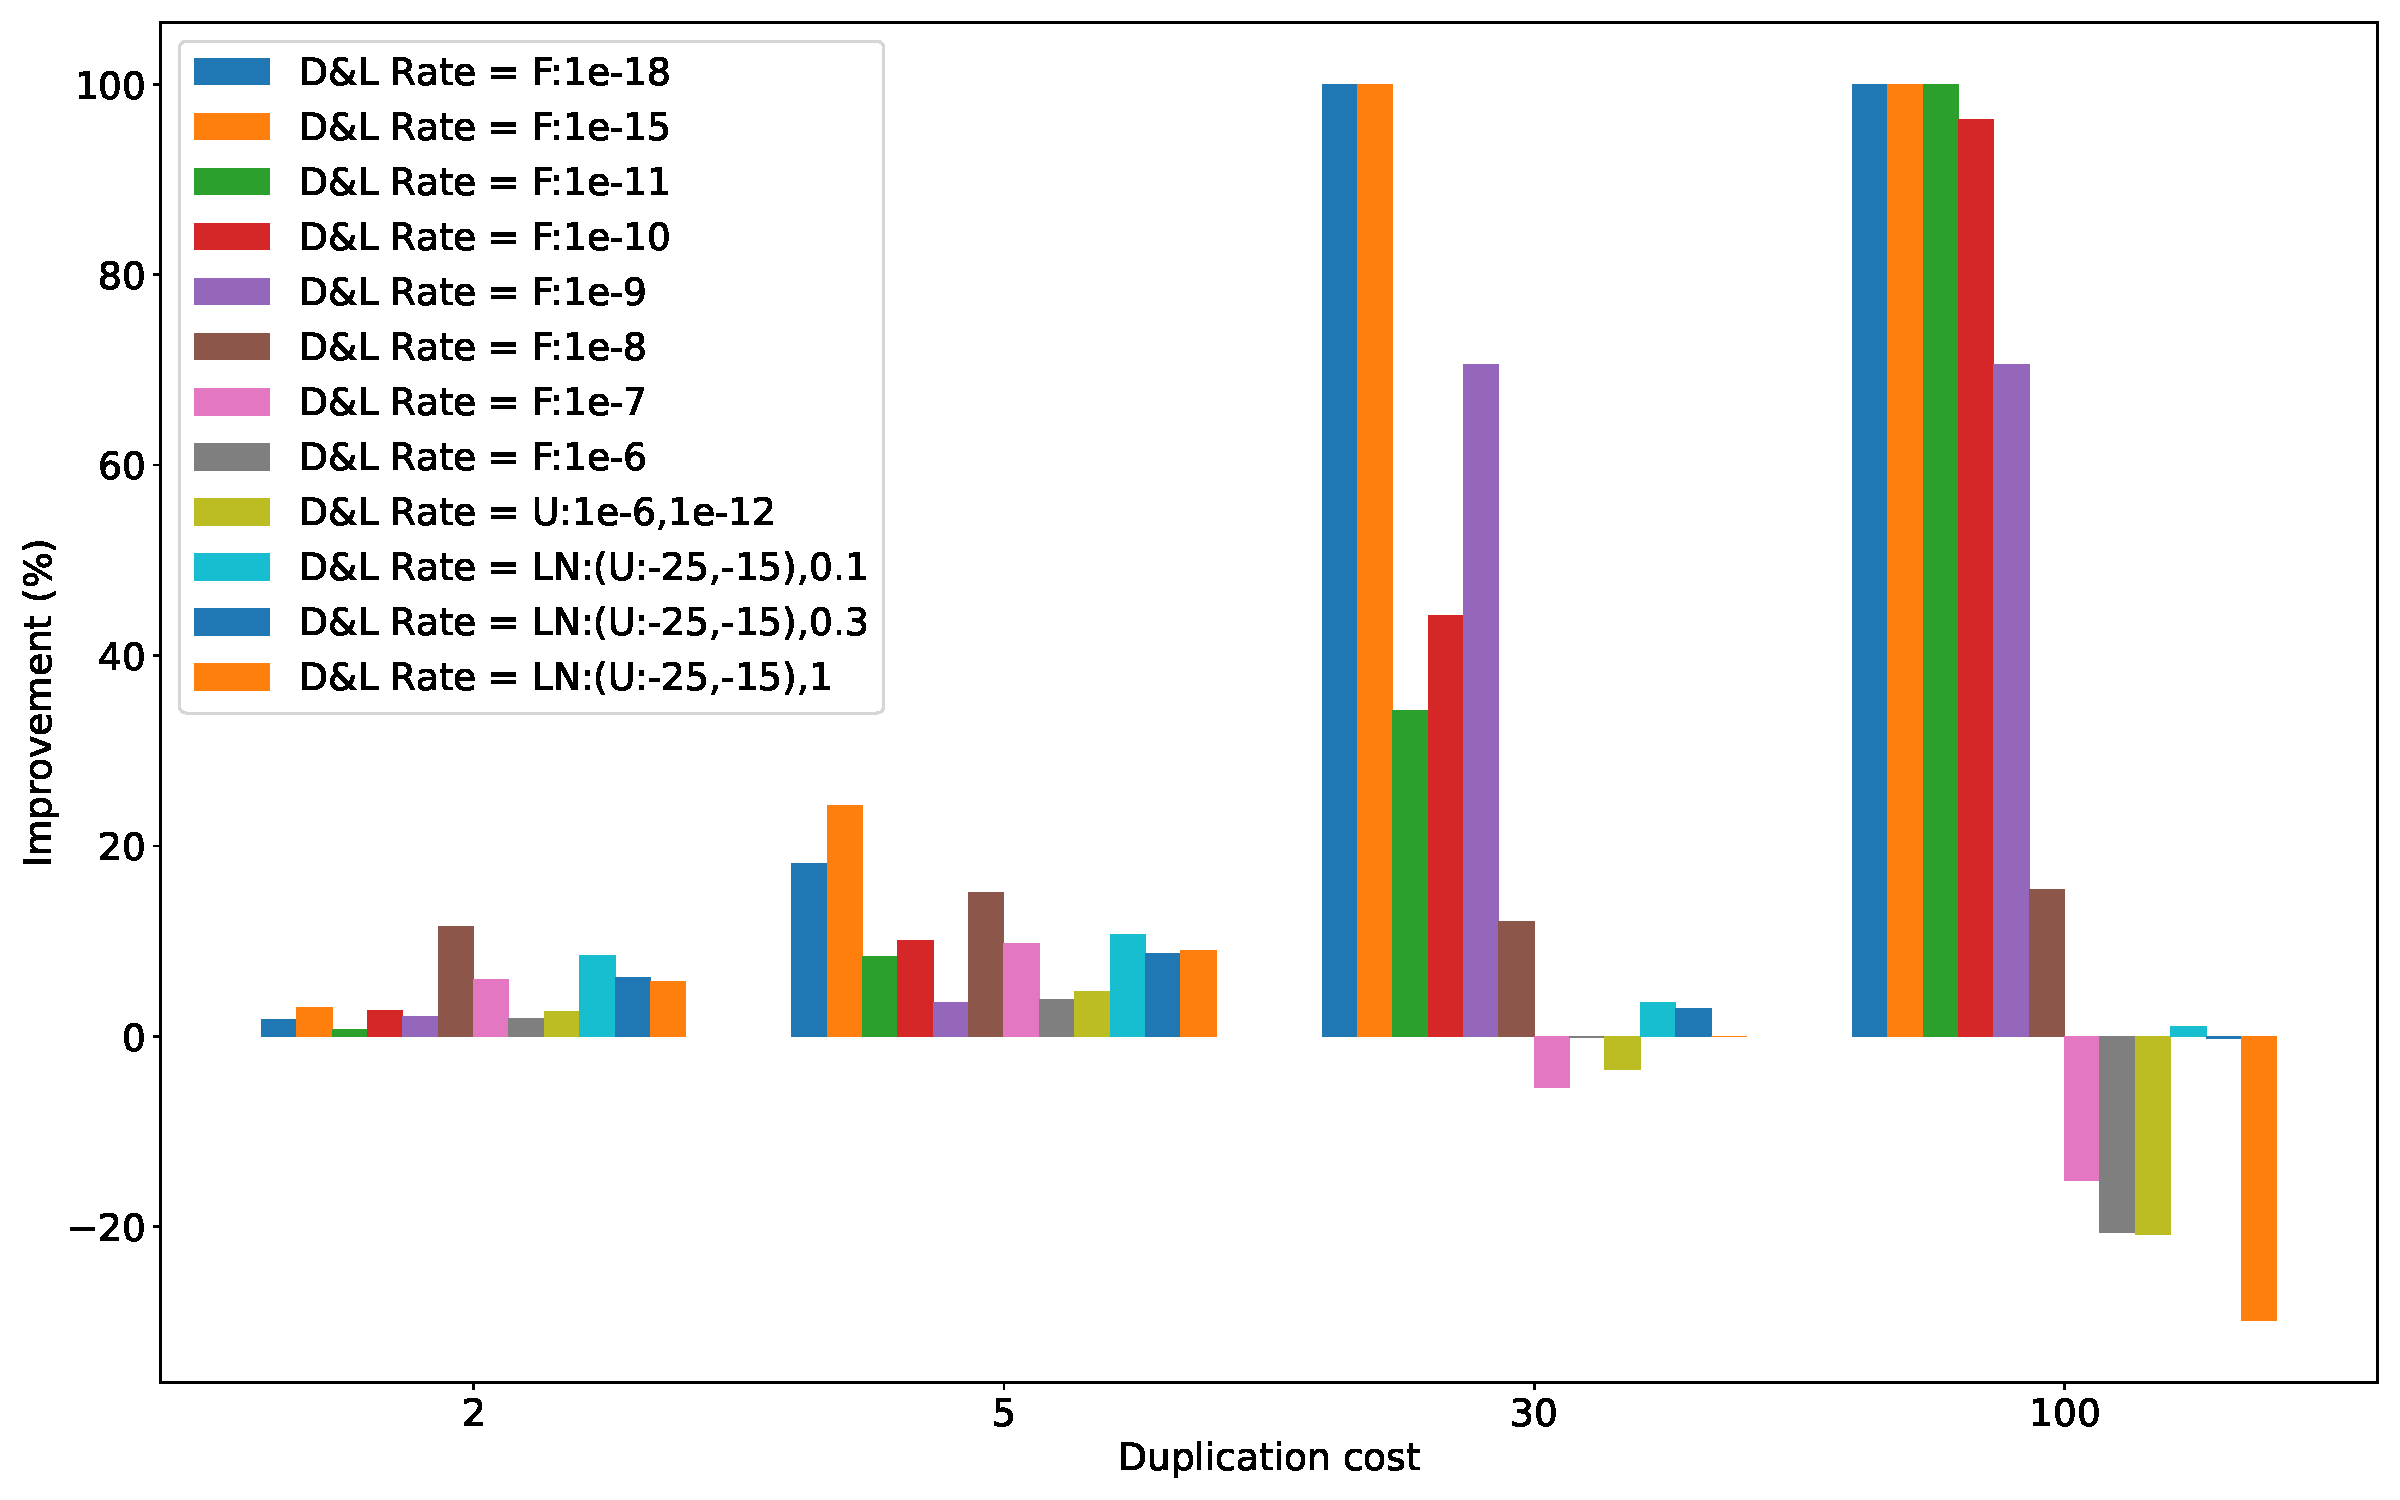
\includegraphics[width=\textwidth]{figs_shortversion/imp_1WGD.pdf} % Adjusted width
        \caption{Improvement percentages for SimPhy simulations, each simulation containing exactly one WGD.}
        \label{fig:imp}
    \end{subfigure}
    \hfill
    \begin{subfigure}[t]{0.41\textwidth}
        \centering
        \raisebox{35pt}{ % Move the figure up by adjusting this value
            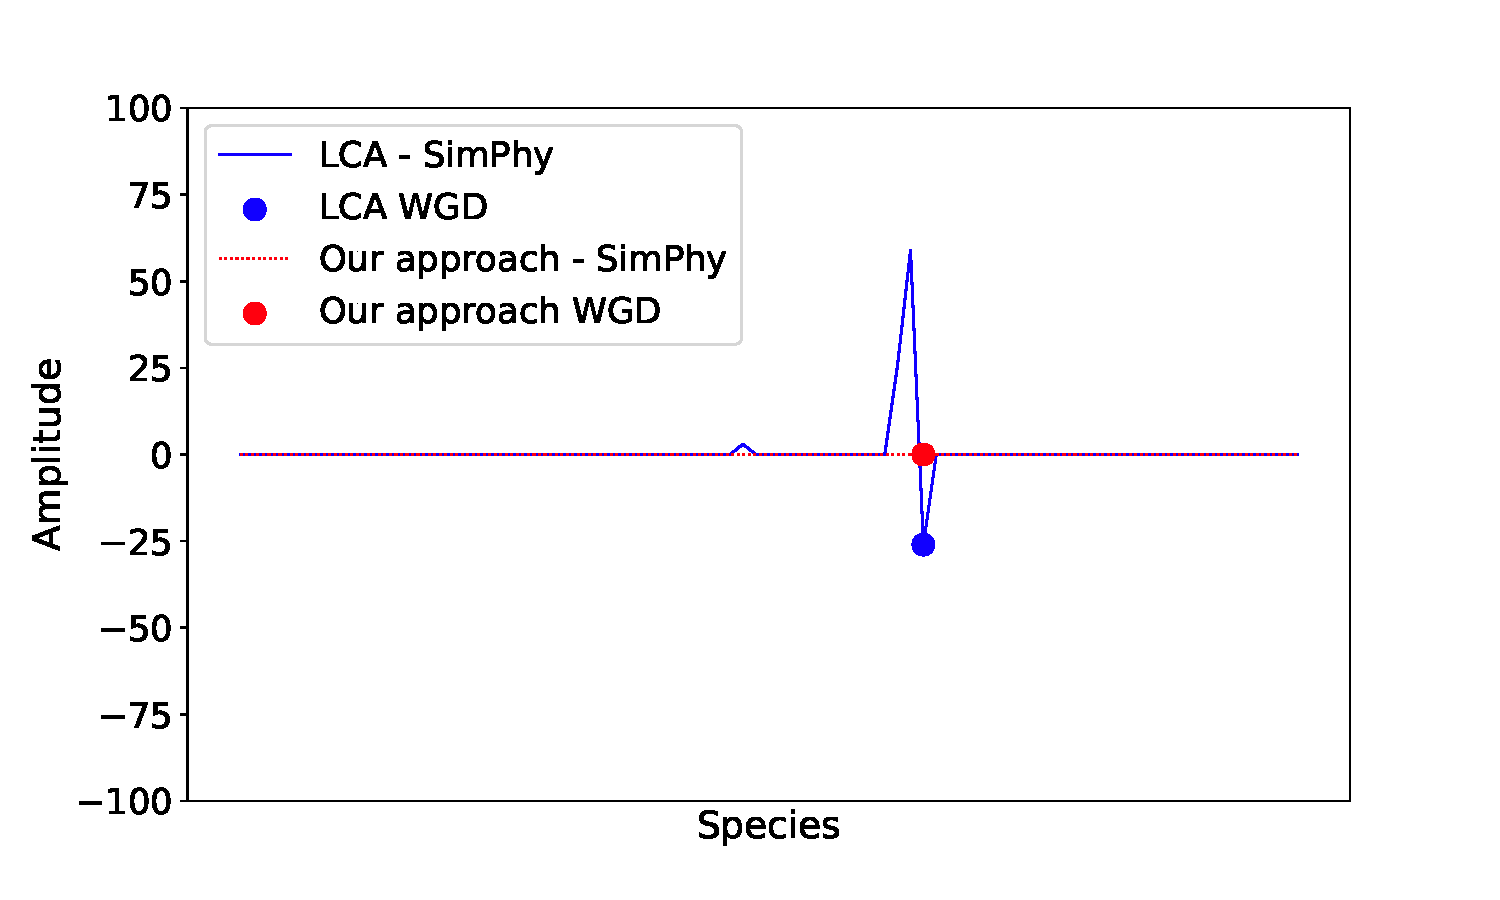
\includegraphics[width=\textwidth]{figs_shortversion/amp-92.pdf}
        }
        \caption{Amplitude}
        \label{fig:amp}
    \end{subfigure}

    \caption{Improvement percentages and amplitude}
    \label{fig:imp_amp}
\end{figure}





\begin{figure}[h!]
    \centering
    % First subplot at the top
    \begin{subfigure}[b]{0.48\textwidth}
        \centering
        %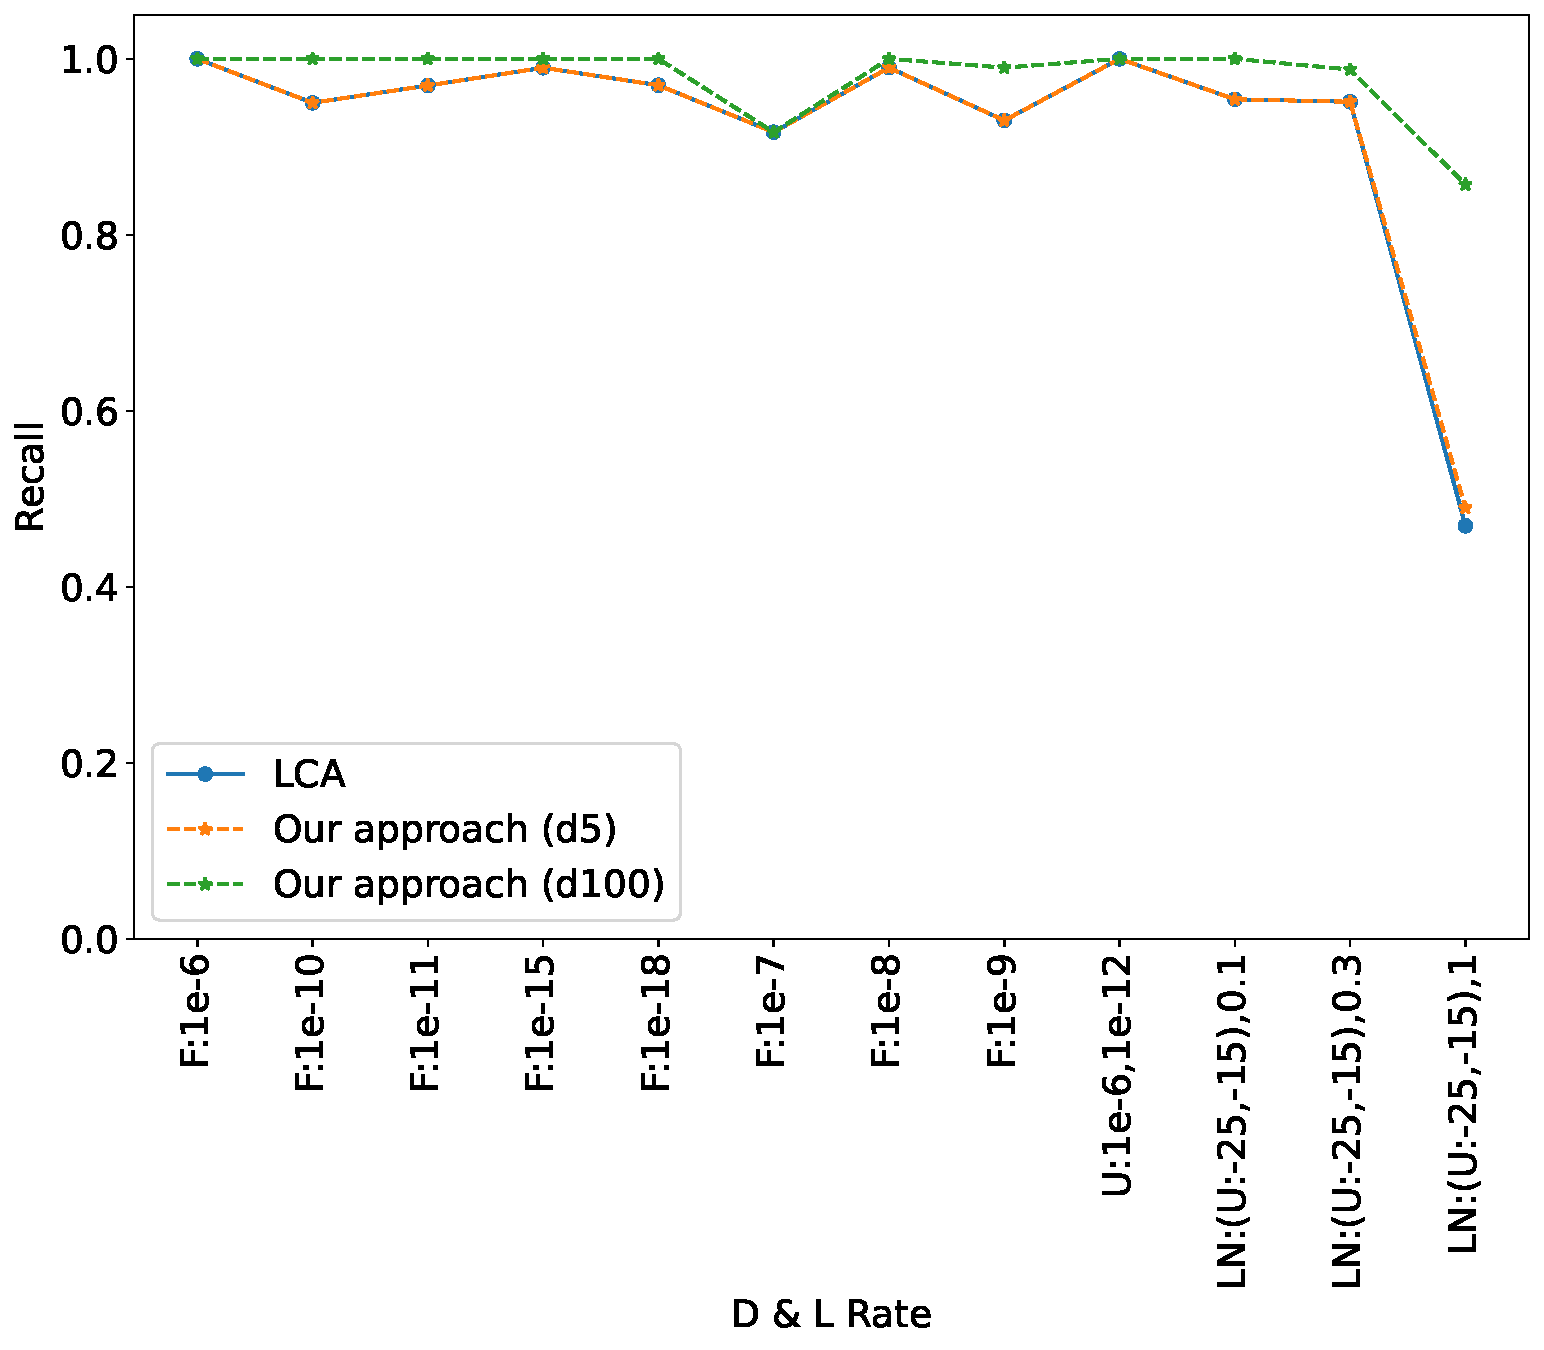
\includegraphics[width=\textwidth]{figs_shortversion/recall-WGD-t10-t80-Avg.pdf}
        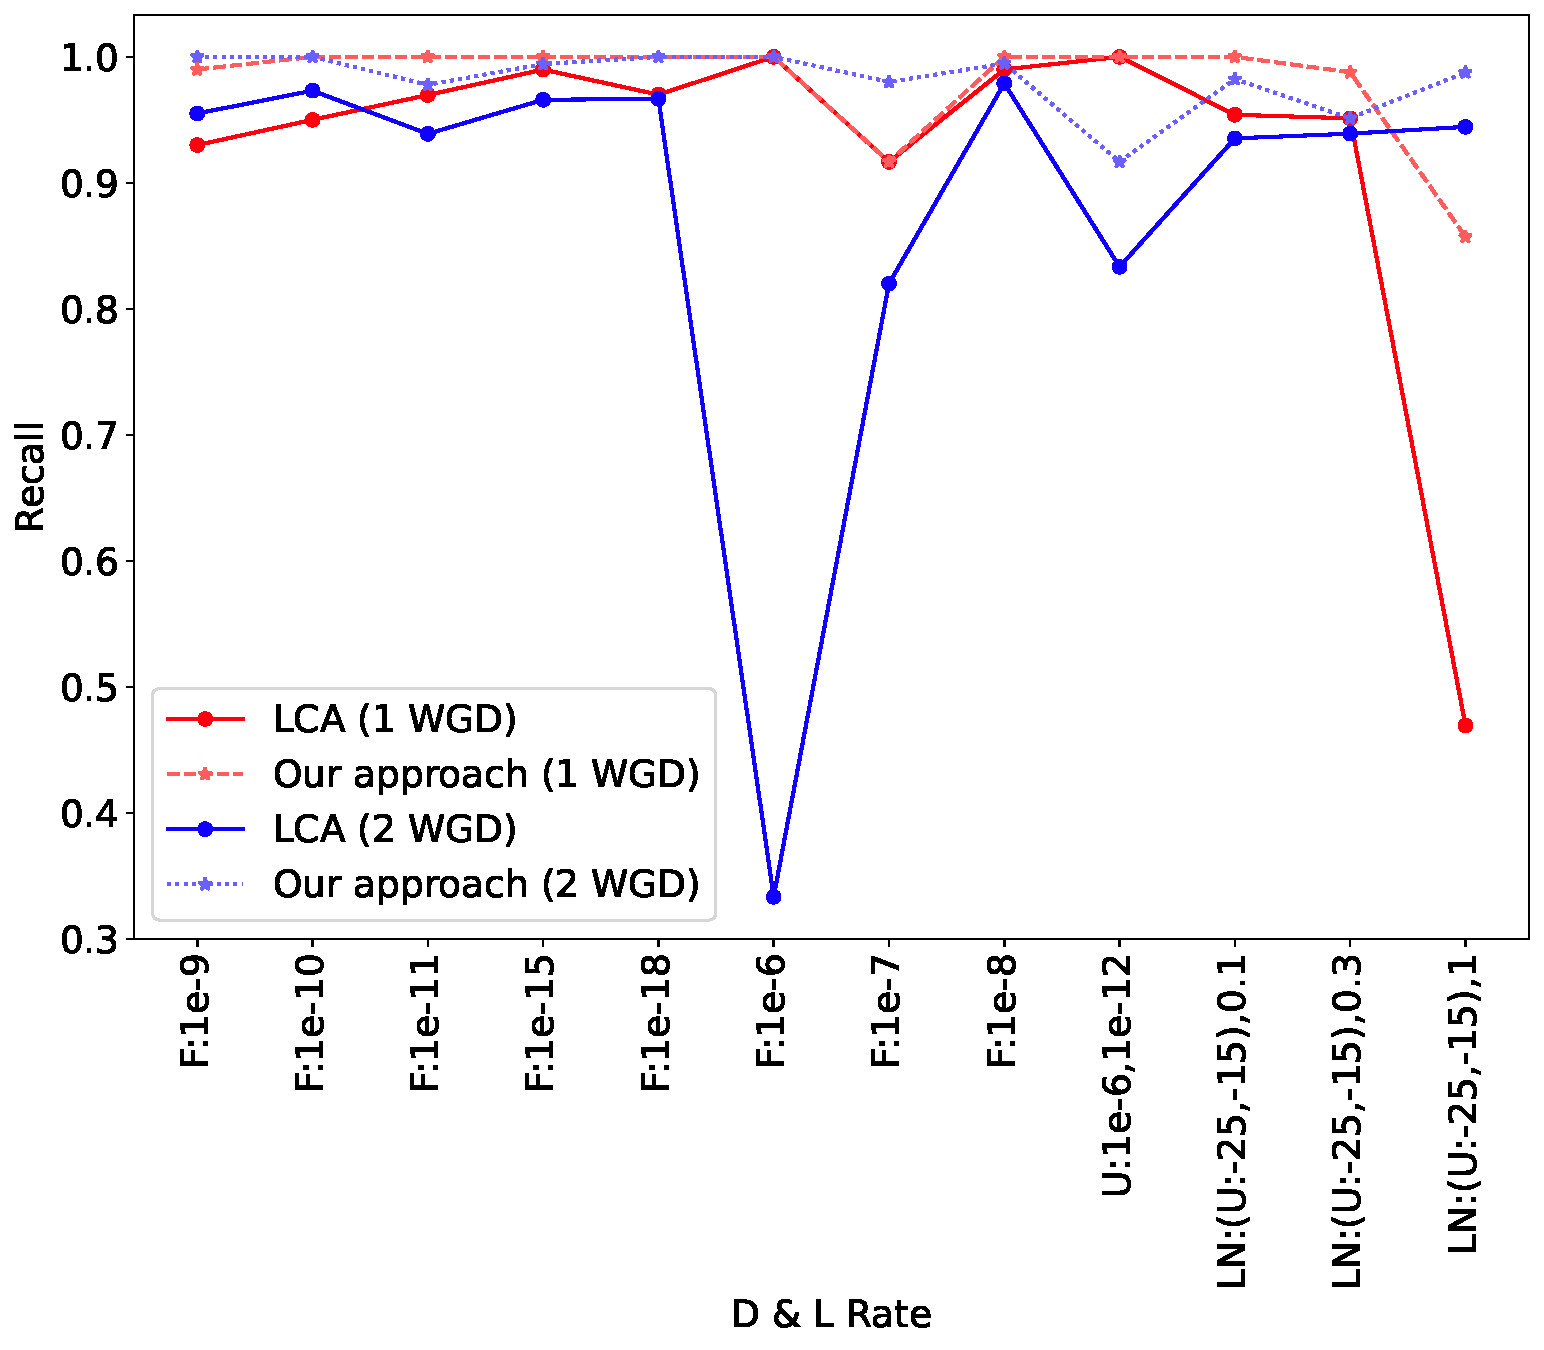
\includegraphics[width=\textwidth]{figs_shortversion/recall-WGD-t10-t80-Avg_recall-2W-WGD-t20-t80-Avg.pdf}
        \caption{Recall of WGD for simulations with 1 WGD and 2 WGD, averaged over 100 runs.}
        \label{fig:recall-wgd-1wgd}
    \end{subfigure}
    \hfill
    % Two subplots in the second row
    \begin{subfigure}[b]{0.48\textwidth}
        \centering
        %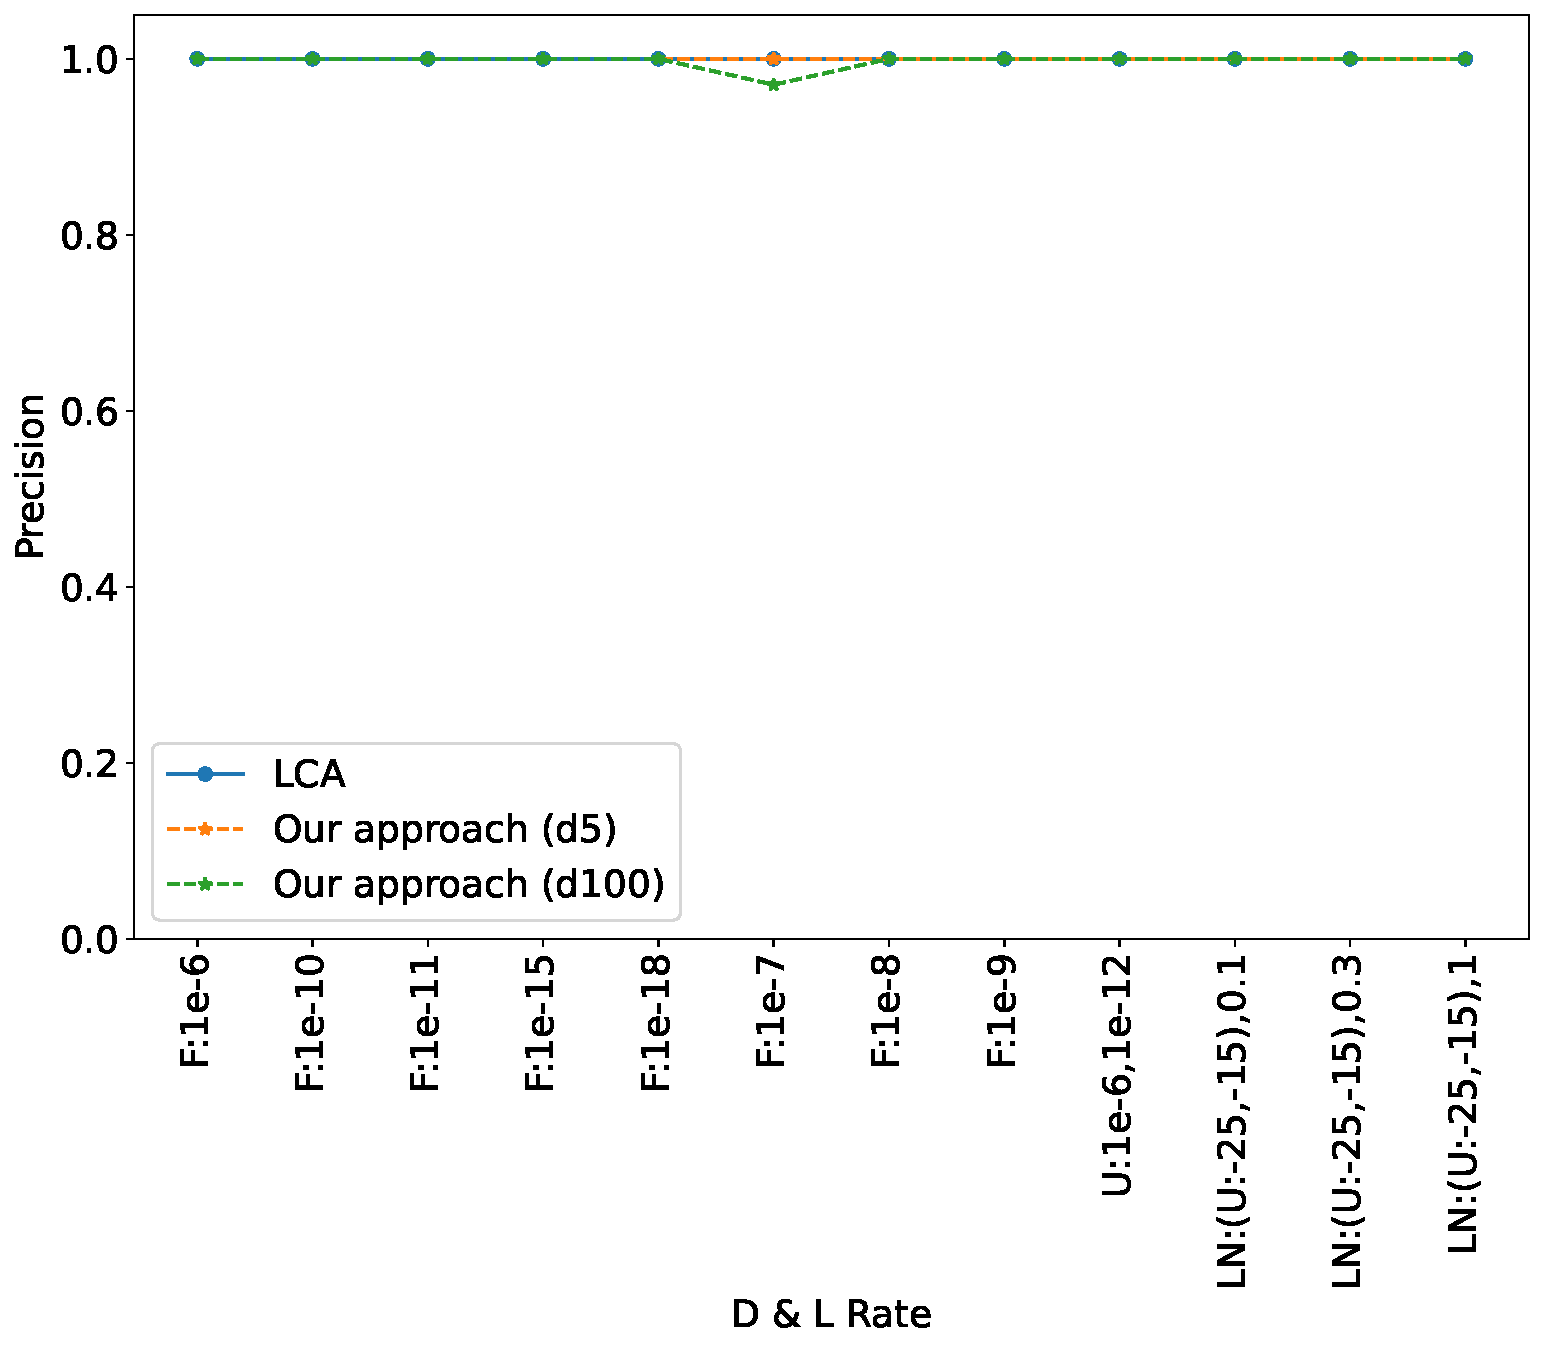
\includegraphics[width=\textwidth]{figs_shortversion/precision-WGD-t10-t80-Avg.pdf}
        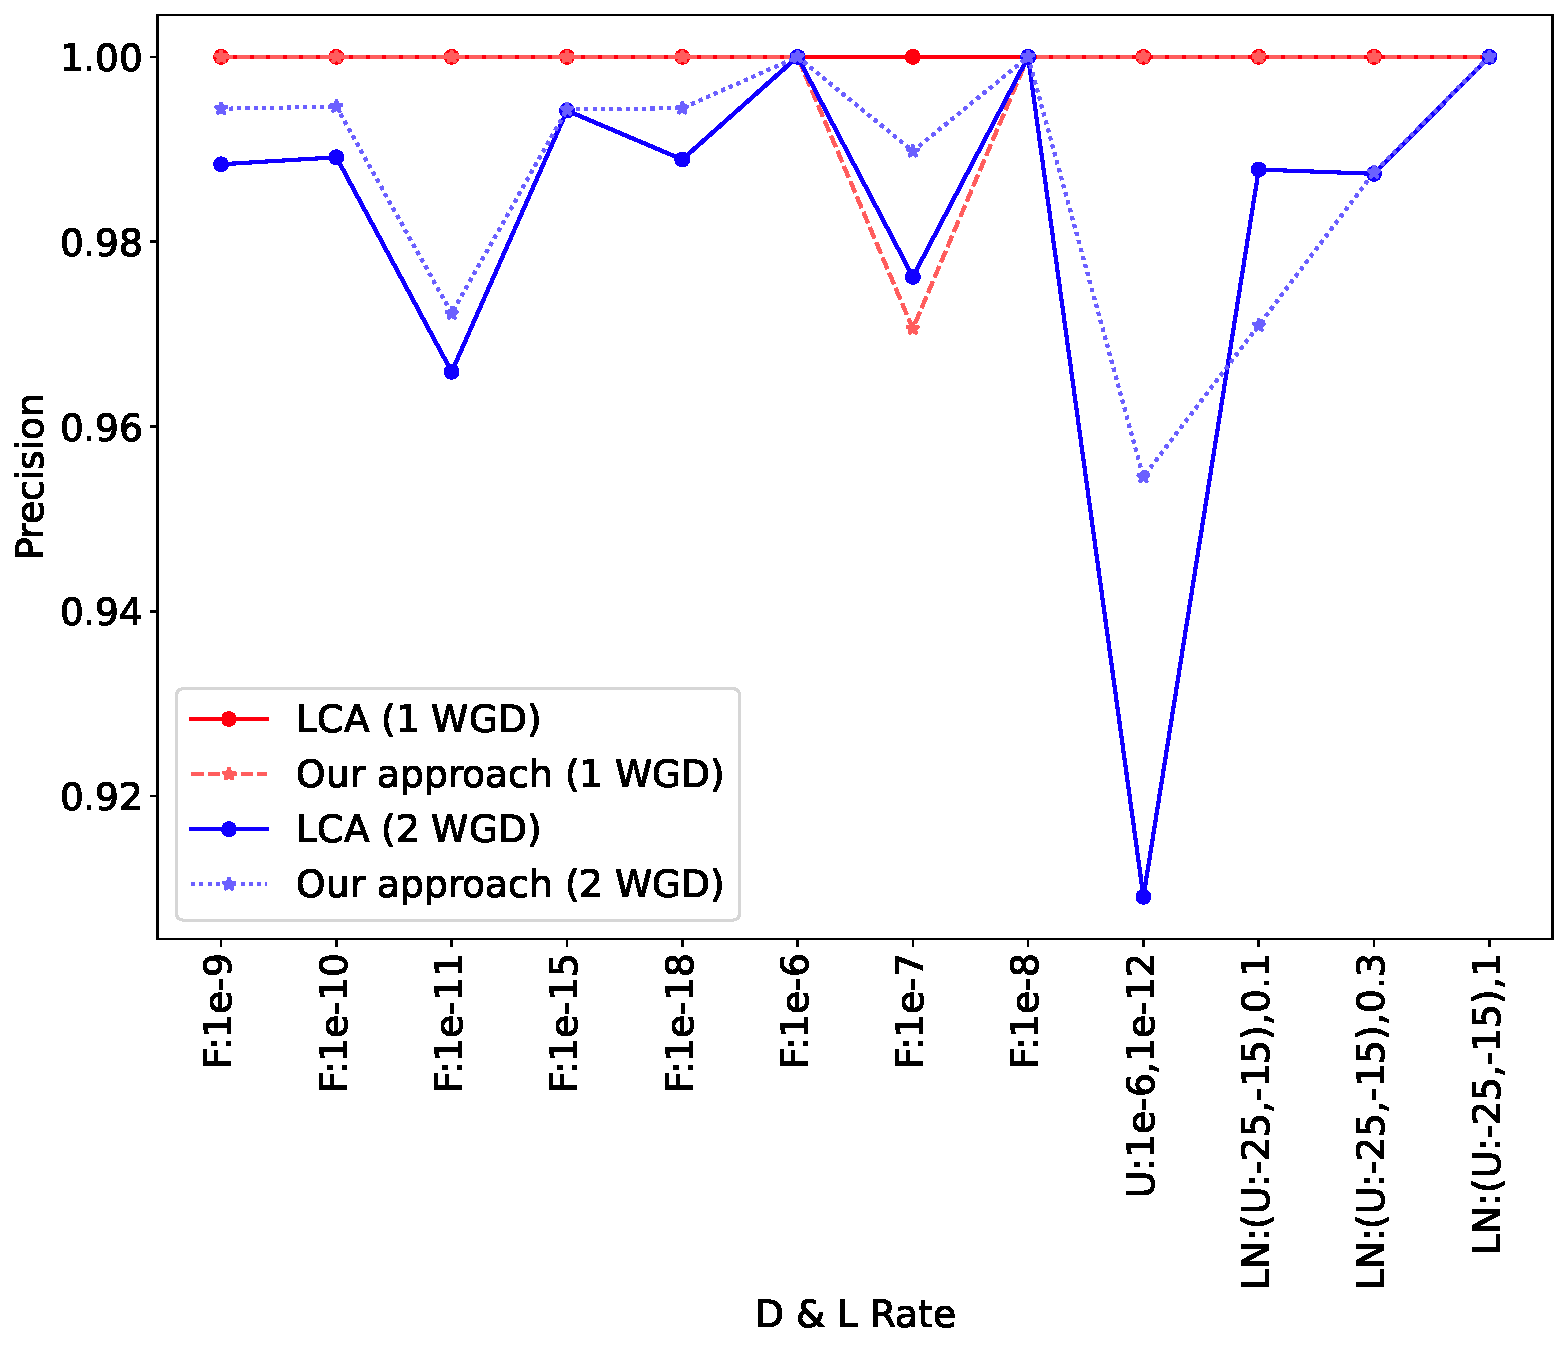
\includegraphics[width=\textwidth]{figs_shortversion/precision-WGD-t10-t80-Avg_precision-2W-WGD-t20-t80-Avg.pdf}
        \caption{Precision of WGD for simulations with 1 WGD and 2 WGD, averaged over 100 runs.}
        \label{fig:precision-wgd-1wgd}
    \end{subfigure}
    
    \caption{
Recall and Precision metrics for detecting WGD events in simulations containing either one WGD or two, analyzed under varying duplication and loss rates. Each result is an average derived from 100 simulation runs, ensuring reliability and robustness of the findings. Subfigure (a) shows the Recall metric, (b) displays the Precision metric.
    }
    \label{fig:recall-precision-wgd}
\end{figure}


\subsection{Results on real datasets}

\ml{[describe datasets we used, with references, and show differences between us and lca.]}
The first dataset we analyzed consists of 53 gene trees from 16 eukaryote species, introduced by Guigó et al. in \cite{guigo1996reconstruction} and previously analyzed in \cite{bansal2008multiple, page2001vertebrate, dondi2019reconciling}. In Figure \ref{fig:guigo}, each internal node is labeled as A/B, where A is the node ID, and B represents the number of gene trees supporting duplications at that species. In \cite{guigo1996reconstruction}, four segmental duplications were identified at nodes 6, 22, 28, and 30, supported by 6, 17, 9, and 13 gene trees, respectively. Additionally, two consecutive segmental duplications were observed at node 28.

Figure \ref{fig:guigo-greedy} shows that our method detects the same segmental duplications at nodes 6, 22, 28 (including two consecutive duplications), and 30, with the same number of supporting gene trees as reported in \cite{guigo1996reconstruction}, using a setup where $\delta = 50$ and $\lambda = 1$. While, Figure \ref{fig:guigo-lca} shows that the LCA method incorrectly identifies nodes 12 and 26 as segmental duplications. Additionally, the previous approach in \cite{dondi2019reconciling} missed node 6 as a segmental duplication.


\begin{figure}[h!]
    \centering

    % Two subplots in the second row
    \begin{subfigure}[b]{0.48\textwidth}
        \centering
        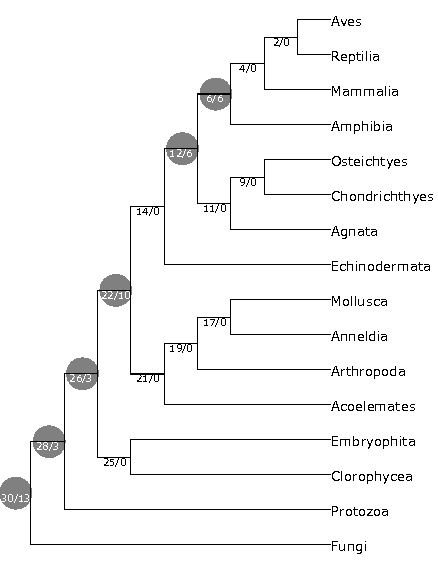
\includegraphics[scale=0.7]{figs_shortversion/guigo_lca.pdf} % Scale down the image
        \caption{Segmental duplications detected by LCA shown as gray circles.}
        \label{fig:guigo-lca}
    \end{subfigure}
    \hfill
    \begin{subfigure}[b]{0.48\textwidth}
        \centering
        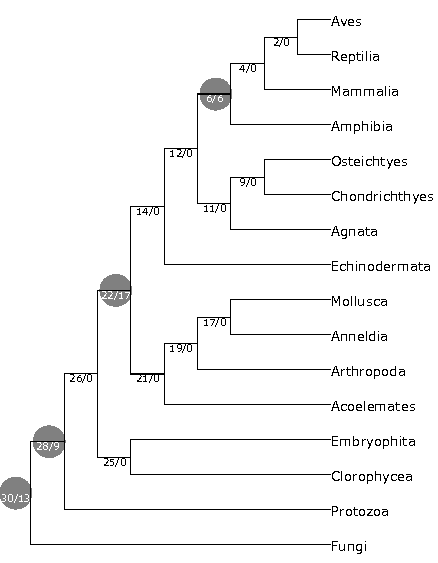
\includegraphics[scale=0.7]{figs_shortversion/guigo_greedy50.pdf} % Scale down the image
        \caption{Segmental duplications detected by our algorithm ($\delta=50$, $\lambda=1$) shown as gray circles.}
        \label{fig:guigo-greedy}
    \end{subfigure}
    
    \caption{
        Species tree of 16 eukaryotes studied by Guigó et al for 53 gene trees. Each node is labeled with two numbers (A/B), where A is the node ID and B is the number of gene trees supporting duplications in that species.
    }
    \label{fig:guigo}
\end{figure}

\subsection{Yeast}
We also analyzed the yeast species dataset, which includes 2,379 gene trees for 16 species, as presented in \cite{butler2009evolution}. To refine unsupported branches, we employed the method detailed in \cite{jacox2017resolution} and implemented in ecceTERA \cite{jacox2016eccetera}, using a bootstrap threshold of 0.9 and setting $\delta = \lambda = 1$. Figure \ref{fig:fungi-greedy} demonstrates that our method identifies two WGDs at nodes 10 and 16, while Figure \ref{fig:fungi-lca} confirms only one WGD at node 10. Additionally, the two segmental duplications at nodes 6 and 29 are consistent between both our algorithm and the LCA method. However, node 15 is identified as a segmental duplication by LCA, while our method relocates these duplications to the parent node, resulting in node 16 being classified as a WGD instead of a segmental duplication. \rk{[Need a discussion for node 16?]}



\begin{figure}[h!]
    \centering

    % Two subplots in the second row
    \begin{subfigure}[b]{0.48\textwidth}
        \centering
        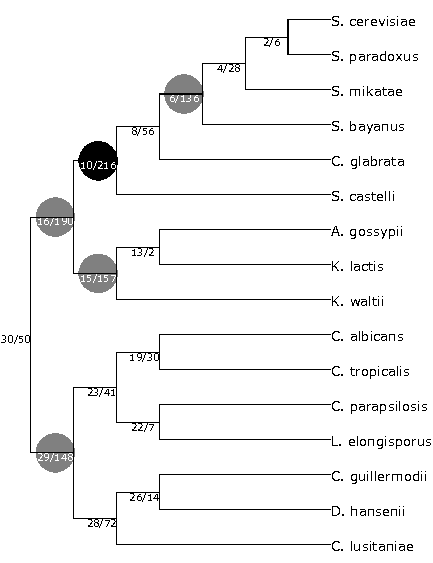
\includegraphics[scale=0.7]{figs/fungi_lca.pdf} % Scale down the image
        \caption{WGD (black cicles) and Segmental duplications (gray circles) detected by LCA.}
        \label{fig:fungi-lca}
    \end{subfigure}
    \hfill
    \begin{subfigure}[b]{0.48\textwidth}
        \centering
        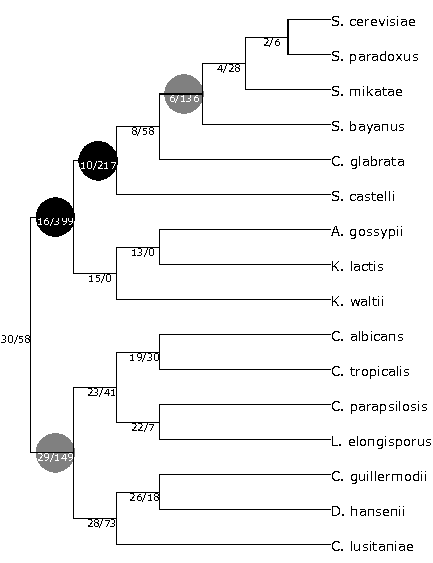
\includegraphics[scale=0.7]{figs/fungi_greedy2000.pdf} % Scale down the image
        \caption{WGD (black cicles) and Segmental duplications (gray circles) detected by our algorithm where $\delta=2000$, $\lambda=1$.}
        \label{fig:fungi-greedy}
    \end{subfigure}
    
    \caption{
        Species tree of 16 yeast species for 2379 gene trees. Each node is labeled with two numbers (A/B), where A is the node ID and B is the count of gene trees supporting duplications in that species.
    }
    \label{fig:fungi}
\end{figure}


\subsection{Fish}
The final dataset we analyzed is from the Atlantic salmon \cite{lien2016atlantic}, sequenced alongside the pike \cite{rondeau2014genome} and rainbow trout \cite{berthelot2014rainbow}. This dataset consists of 12,443 gene trees for 14 species and has been previously studied in \cite{meyer20052r, danzmann2008distribution, hermansen2016extracting}. In Figure \ref{fig:salmon-greedy}, two WGDs are identified at nodes 3 and 24, both of which align with previous findings. While, Figure \ref{fig:salmon-lca} shows that LCA misses the WGD at node 24. \rk{[I couldn't find anything related to the node 18 in the salmon's paper. Only thing I noticed is that in salmon's paper and its citations, they summarize leaves and consider a group of leaves as one leaf.]} 

\begin{figure}[h!]
    \centering

    % Two subplots in the second row
    \begin{subfigure}[b]{0.48\textwidth}
        \centering
        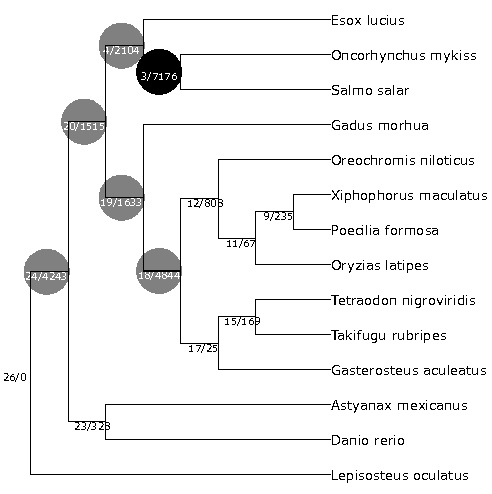
\includegraphics[scale=0.7]{figs/salmon_lca.pdf} % Scale down the image
        \caption{WGD (black cicles) and Segmental duplications (gray circles) detected by LCA.}
        \label{fig:salmon-lca}
    \end{subfigure}
    \hfill
    \begin{subfigure}[b]{0.48\textwidth}
        \centering
        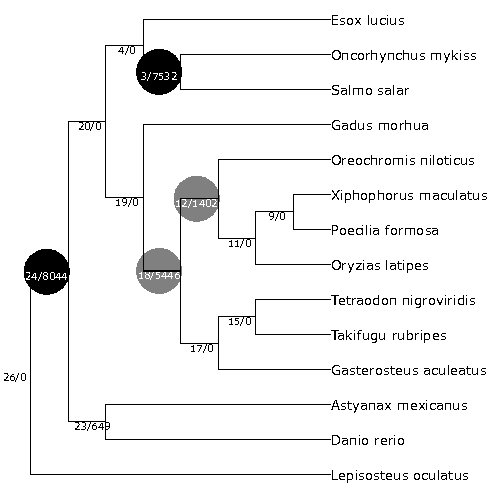
\includegraphics[scale=0.7]{figs/salmon_greedy10000.pdf} % Scale down the image
        \caption{WGD (black cicles) and Segmental duplications (gray circles) detected by our algorithm where $\delta=10000$, $\lambda=1$.}
        \label{fig:salmon-greedy}
    \end{subfigure}
    
    \caption{
        Species tree of atlantic salmon for 12443 gene trees. Each node is labeled with two numbers (A/B), where A is the node ID and B is the count of gene trees supporting duplications in that species.
    }
    \label{fig:salmon}
\end{figure}


\clearpage
\subsection*{Previous stuff}

To begin, we analyze the results from the simulations with one Whole Genome Duplication (WGD) and two WGDs, presented in Figures \ref{fig:imp_1wgd_beforelosses} and \ref{fig:imp_2wgd_beforelosses} respectively. These results are generated under the condition where no losses are applied to the gene trees after the SimPhy simulations, meaning the WGDs remain unaffected by losses. The figures illustrate the improvement percentages across various SimPhy simulations, each subjected to different duplication and loss rates. These results are evaluated under different duplication cost configurations, while keeping the loss cost consistently set to 1.

In the figures, the highest duplication and loss rates tested are $U:1e-6$, $U:1e-12$, and $F:1e-6$, followed by $F:1e-7$. Conversely, the lowest rates are $F:1e-18$, $F:1e-15$, and $F:1e-11$.

In most cases, the LCA mapping outperforms our approach. This is because, when no losses affect the WGDs, the ancestors in the gene trees can be correctly mapped to their respective species, creating an optimal scenario for the LCA method. Additionally, as the duplication cost increases in our approach, it tends to map the gene tree nodes to higher-level species, leading to a decrease in the improvement percentage.

\begin{figure}[hbt!]
    \centering
    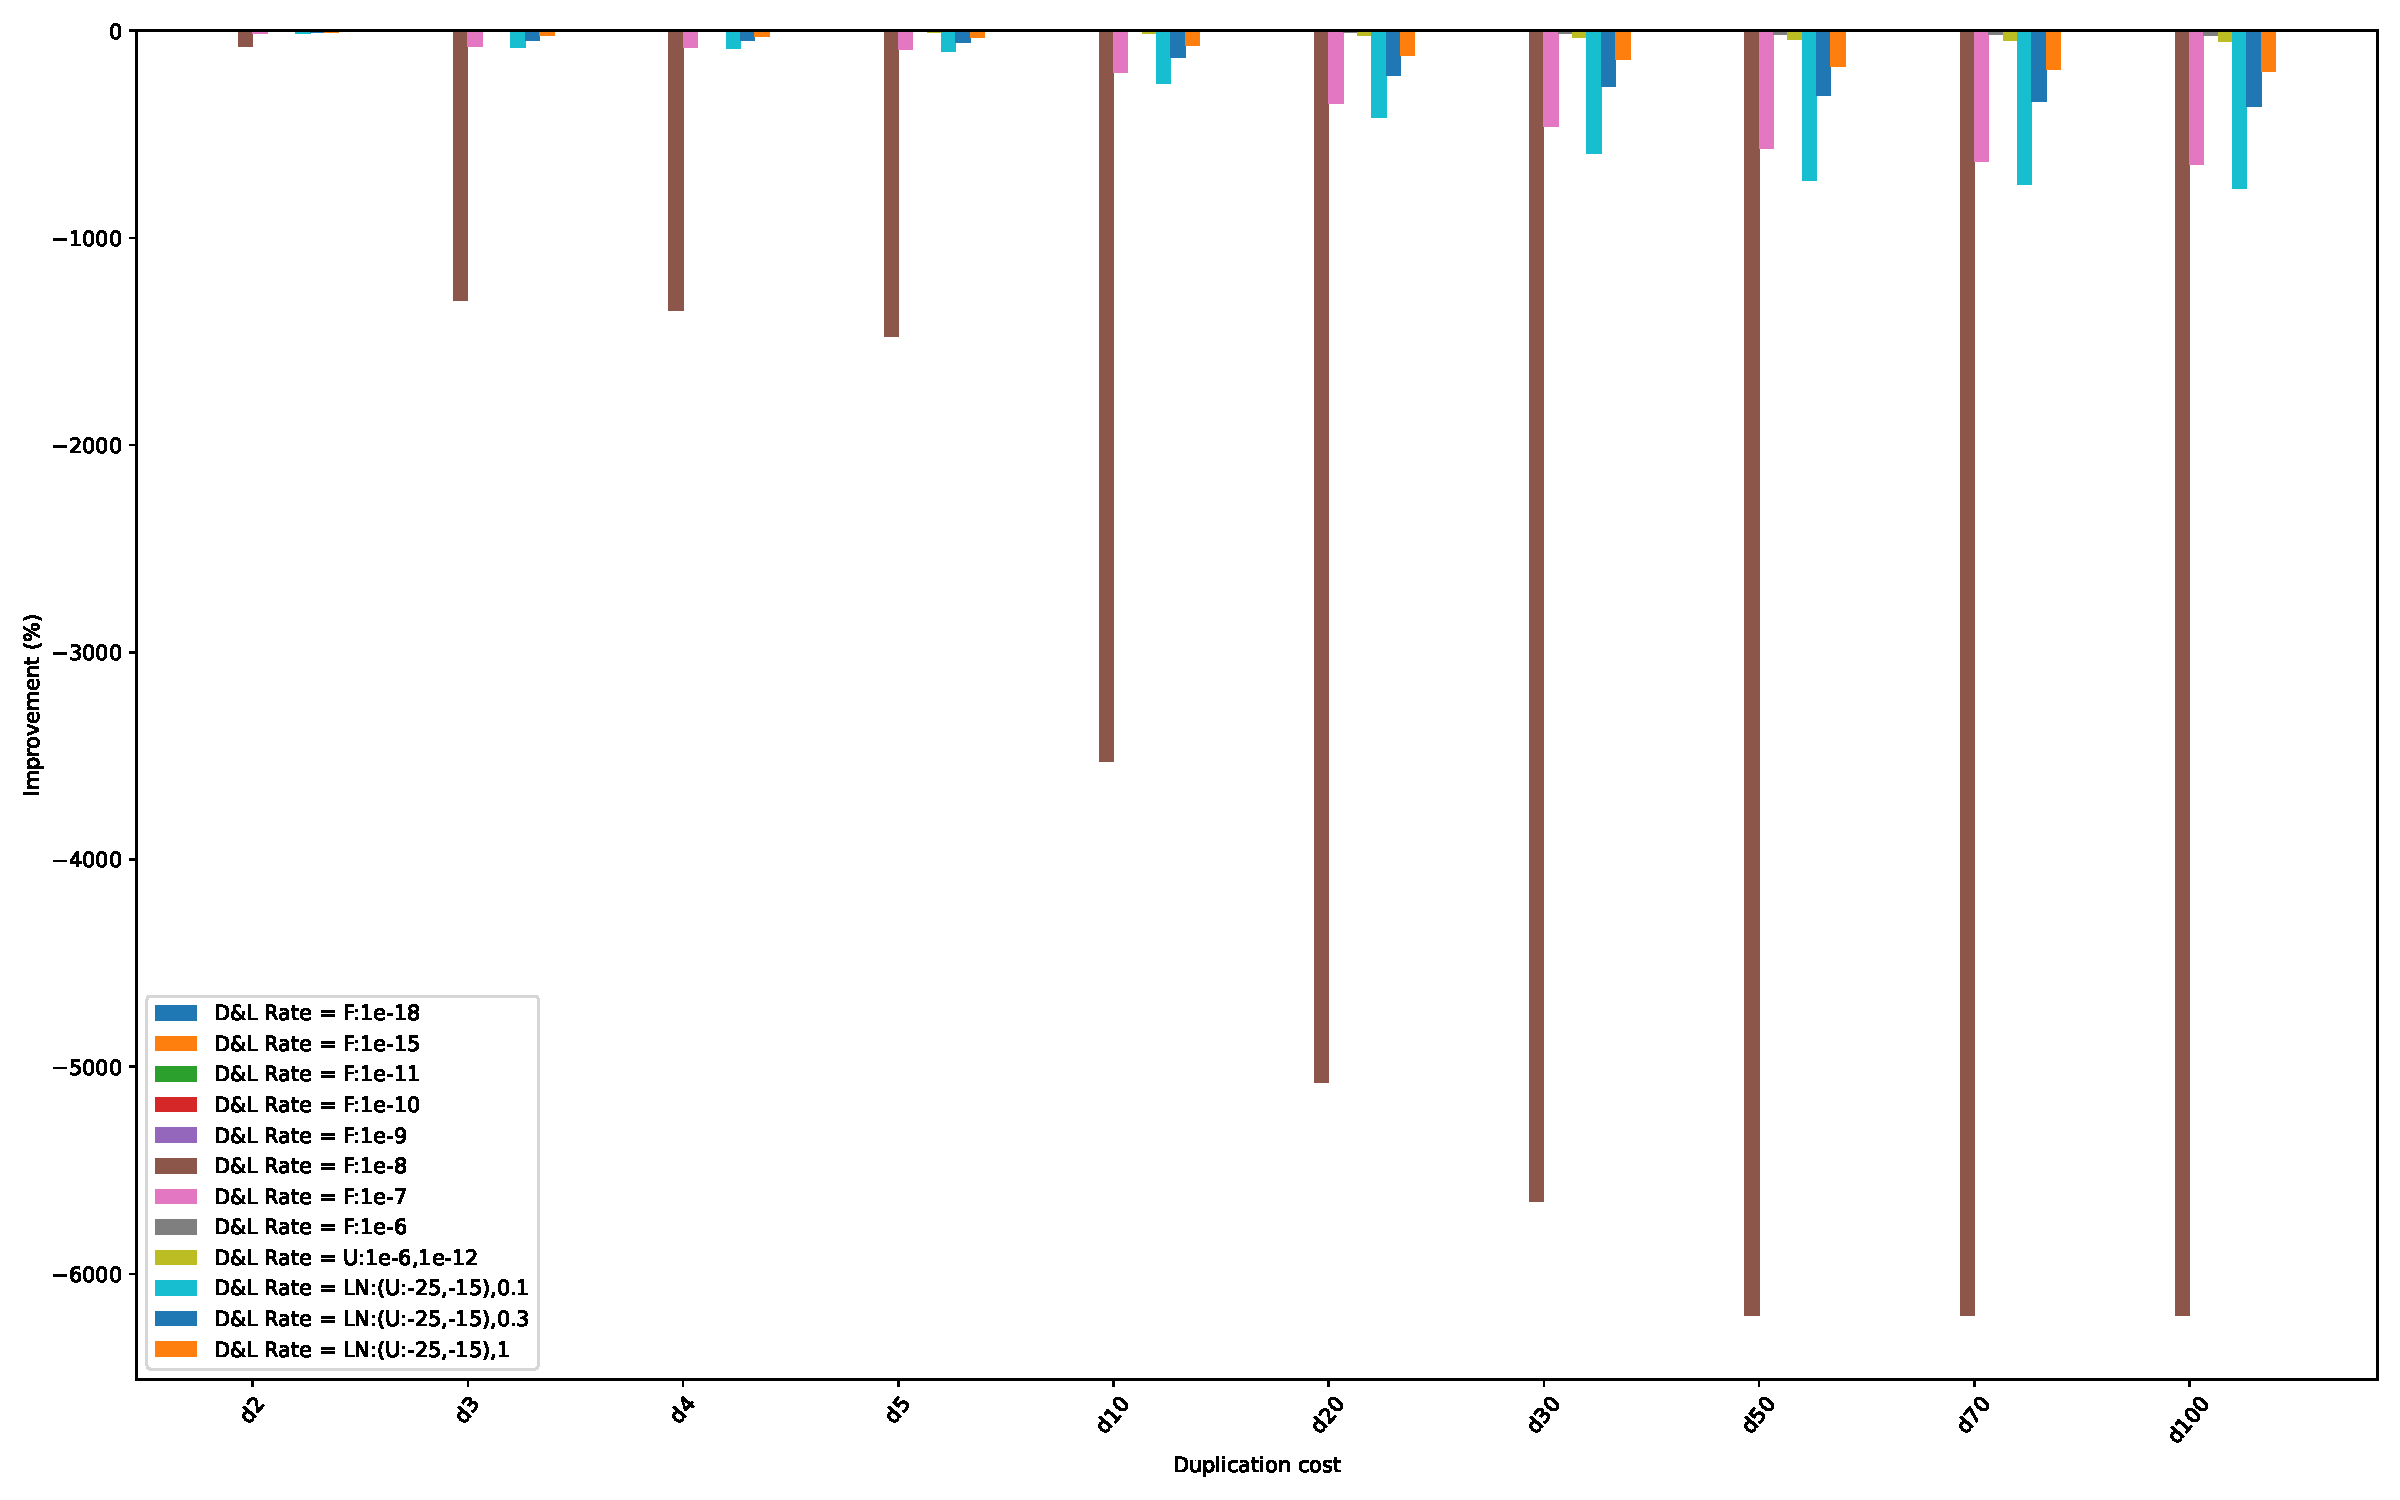
\includegraphics[width=1\textwidth]{figs/imp-1WGD-beforelosses.pdf}
    \caption{Improvement percentages for SimPhy simulations with varying duplication and loss rates. In the legend, "F" represents Point (fixed value) distribution, "U" represents Uniform distribution, and "LN" represents LogUniform distribution. Each simulation includes exactly one WGD event, with no losses applied to the gene trees after the SimPhy simulation.. The x-axis shows the duplication cost used in the algorithm's setup, with the loss cost consistently set to 1.}
    \label{fig:imp_1wgd_beforelosses}
\end{figure}

\begin{figure}[hbt!]
    \centering
    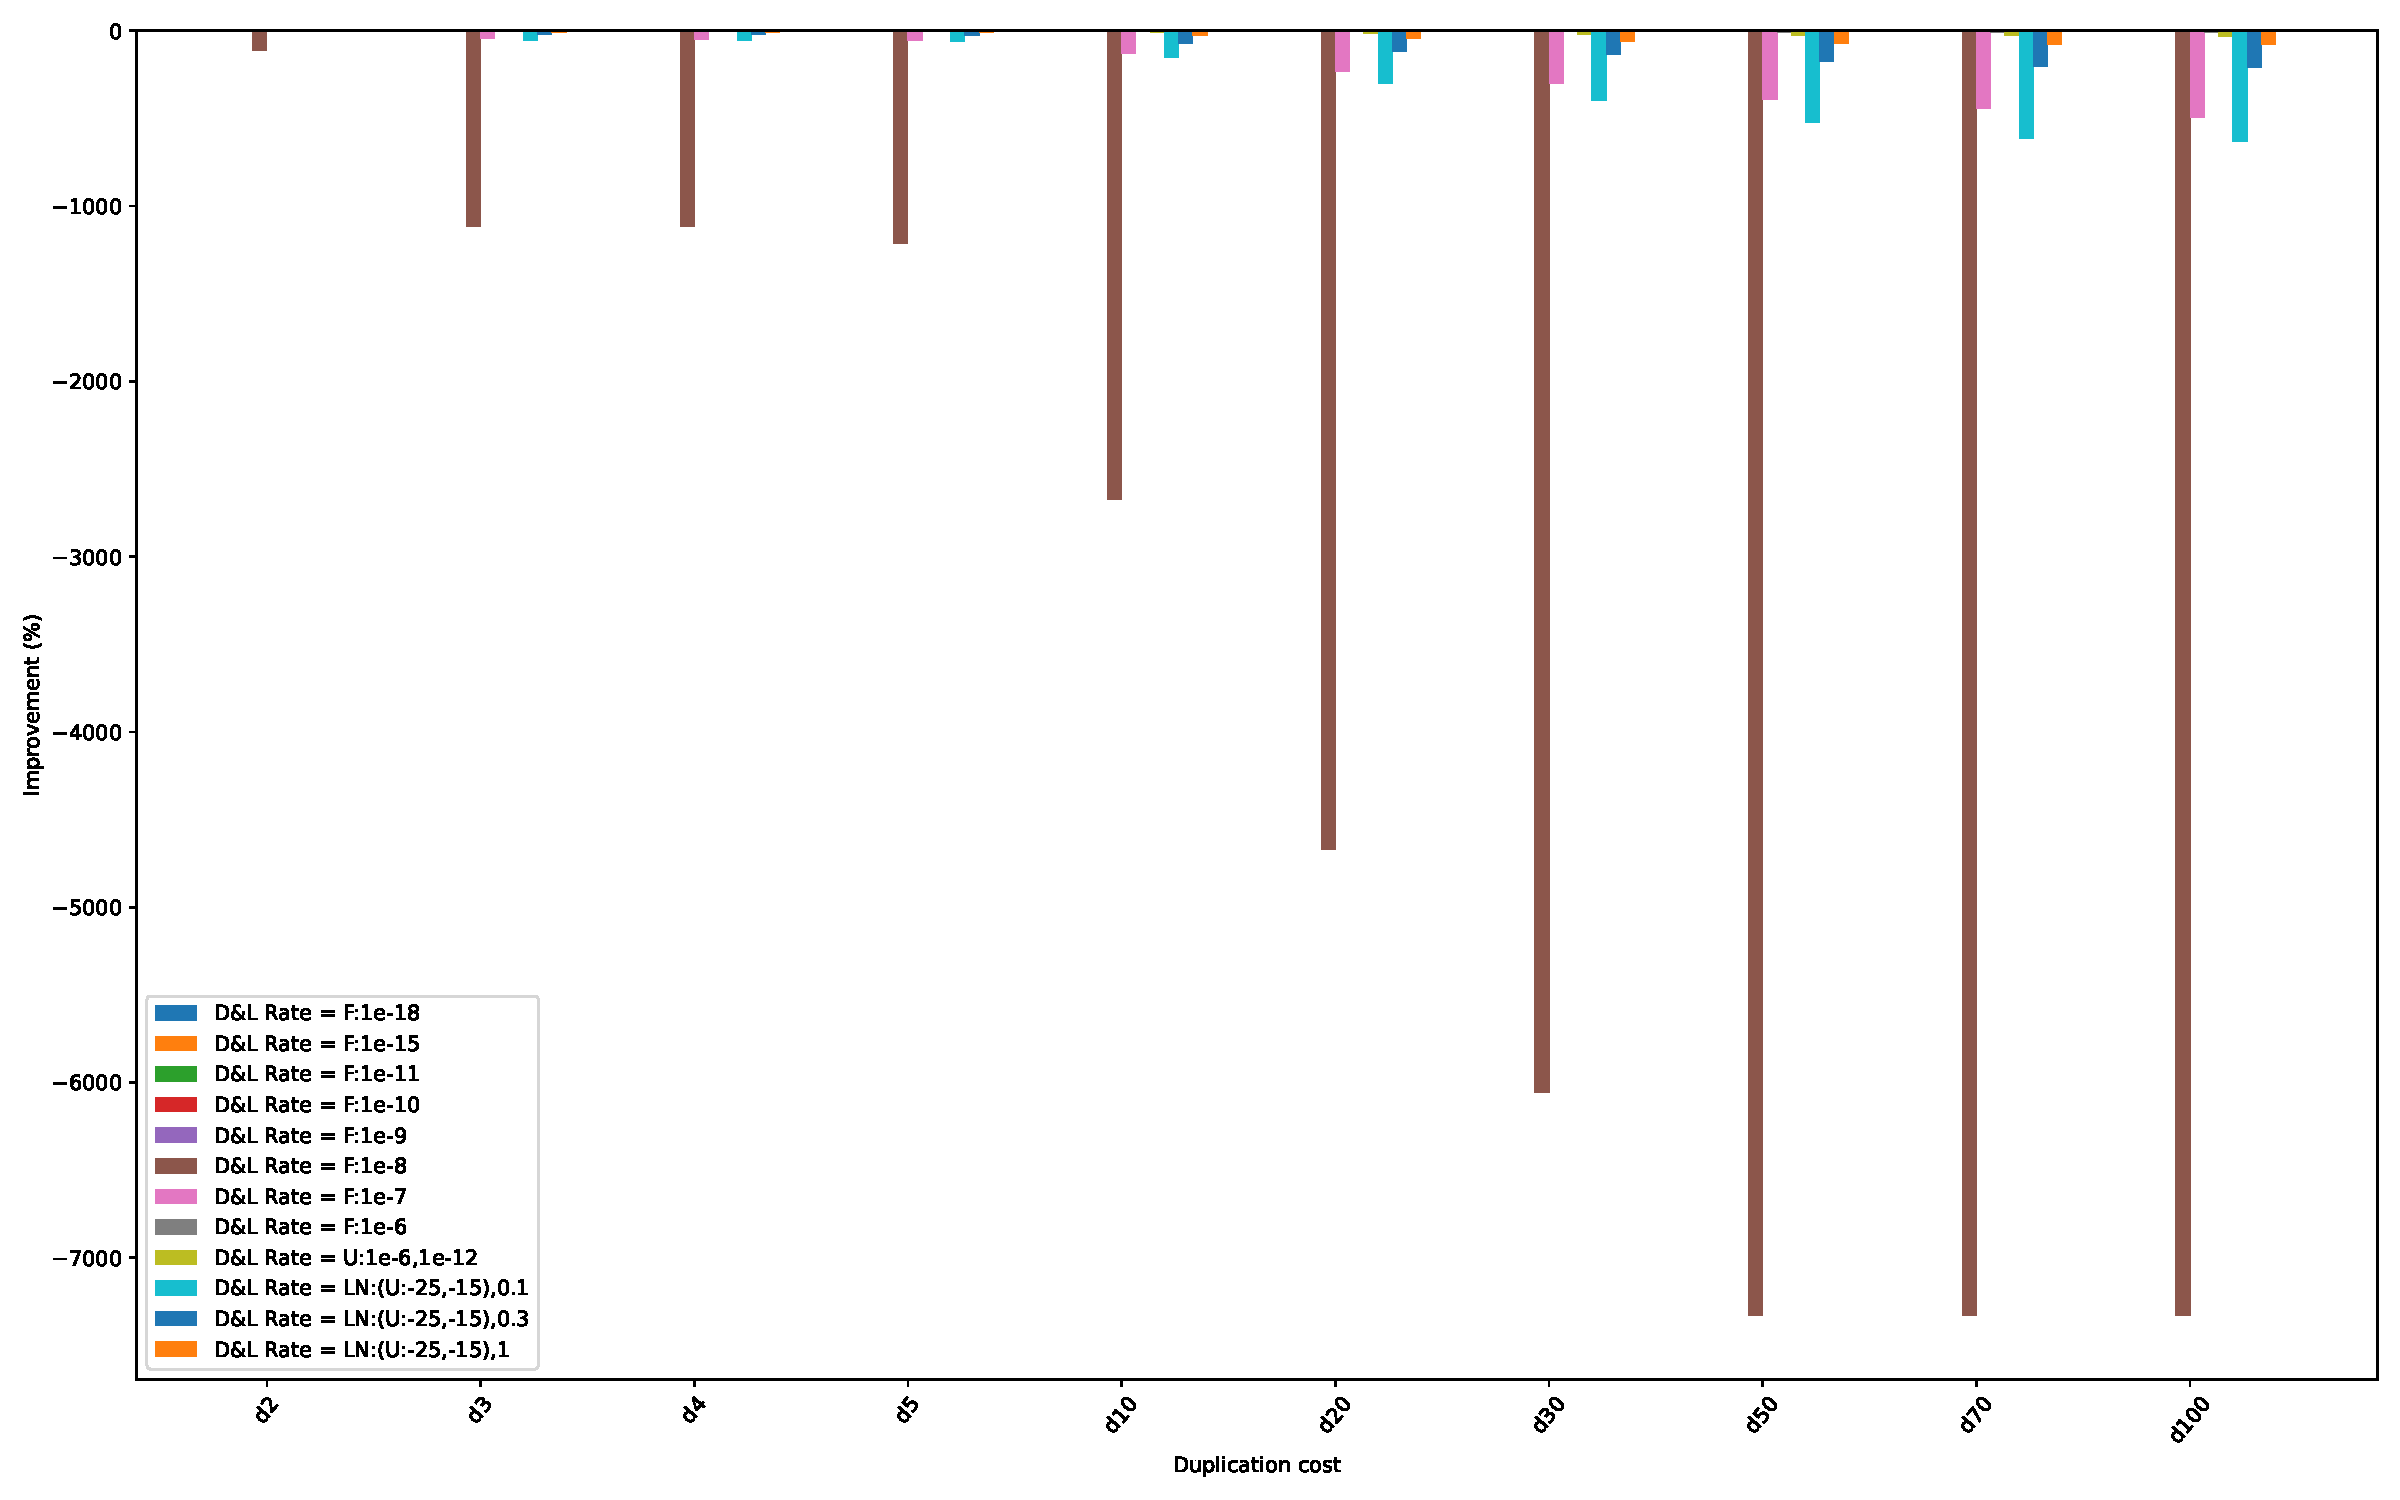
\includegraphics[width=1\textwidth]{figs/imp-2WGD-beforelosses.pdf}
    \caption{Improvement percentages for SimPhy simulations, each containing exactly two WGD events, with no losses applied to the gene trees after the SimPhy simulation.}
    \label{fig:imp_2wgd_beforelosses}
\end{figure}

In Figure \ref{fig:imp_1wgd} and \ref{fig:imp_2wgd}, we examine the results from simulations where losses were applied to the gene trees after SimPhy simulations. The loss rate used is $(n-1)/n$ for each species, where $n$ represents the number of copies of a species. This analysis helps us understand how the application of losses affects the improvement percentages in simulations with one and two WGD events, respectively.

The Figure \ref{fig:imp_1wgd} suggests that with higher duplication costs, the algorithm tends to map duplications to more distant species, leading to greater improvements for lower duplication and loss rates. However, for higher duplication and loss rates, this can result in reduced improvements. Notably, with lower duplication costs (ranging from $d=2$ to $d=20$), the improvements are consistently positive.


\begin{figure}[hbt!]
    \centering
    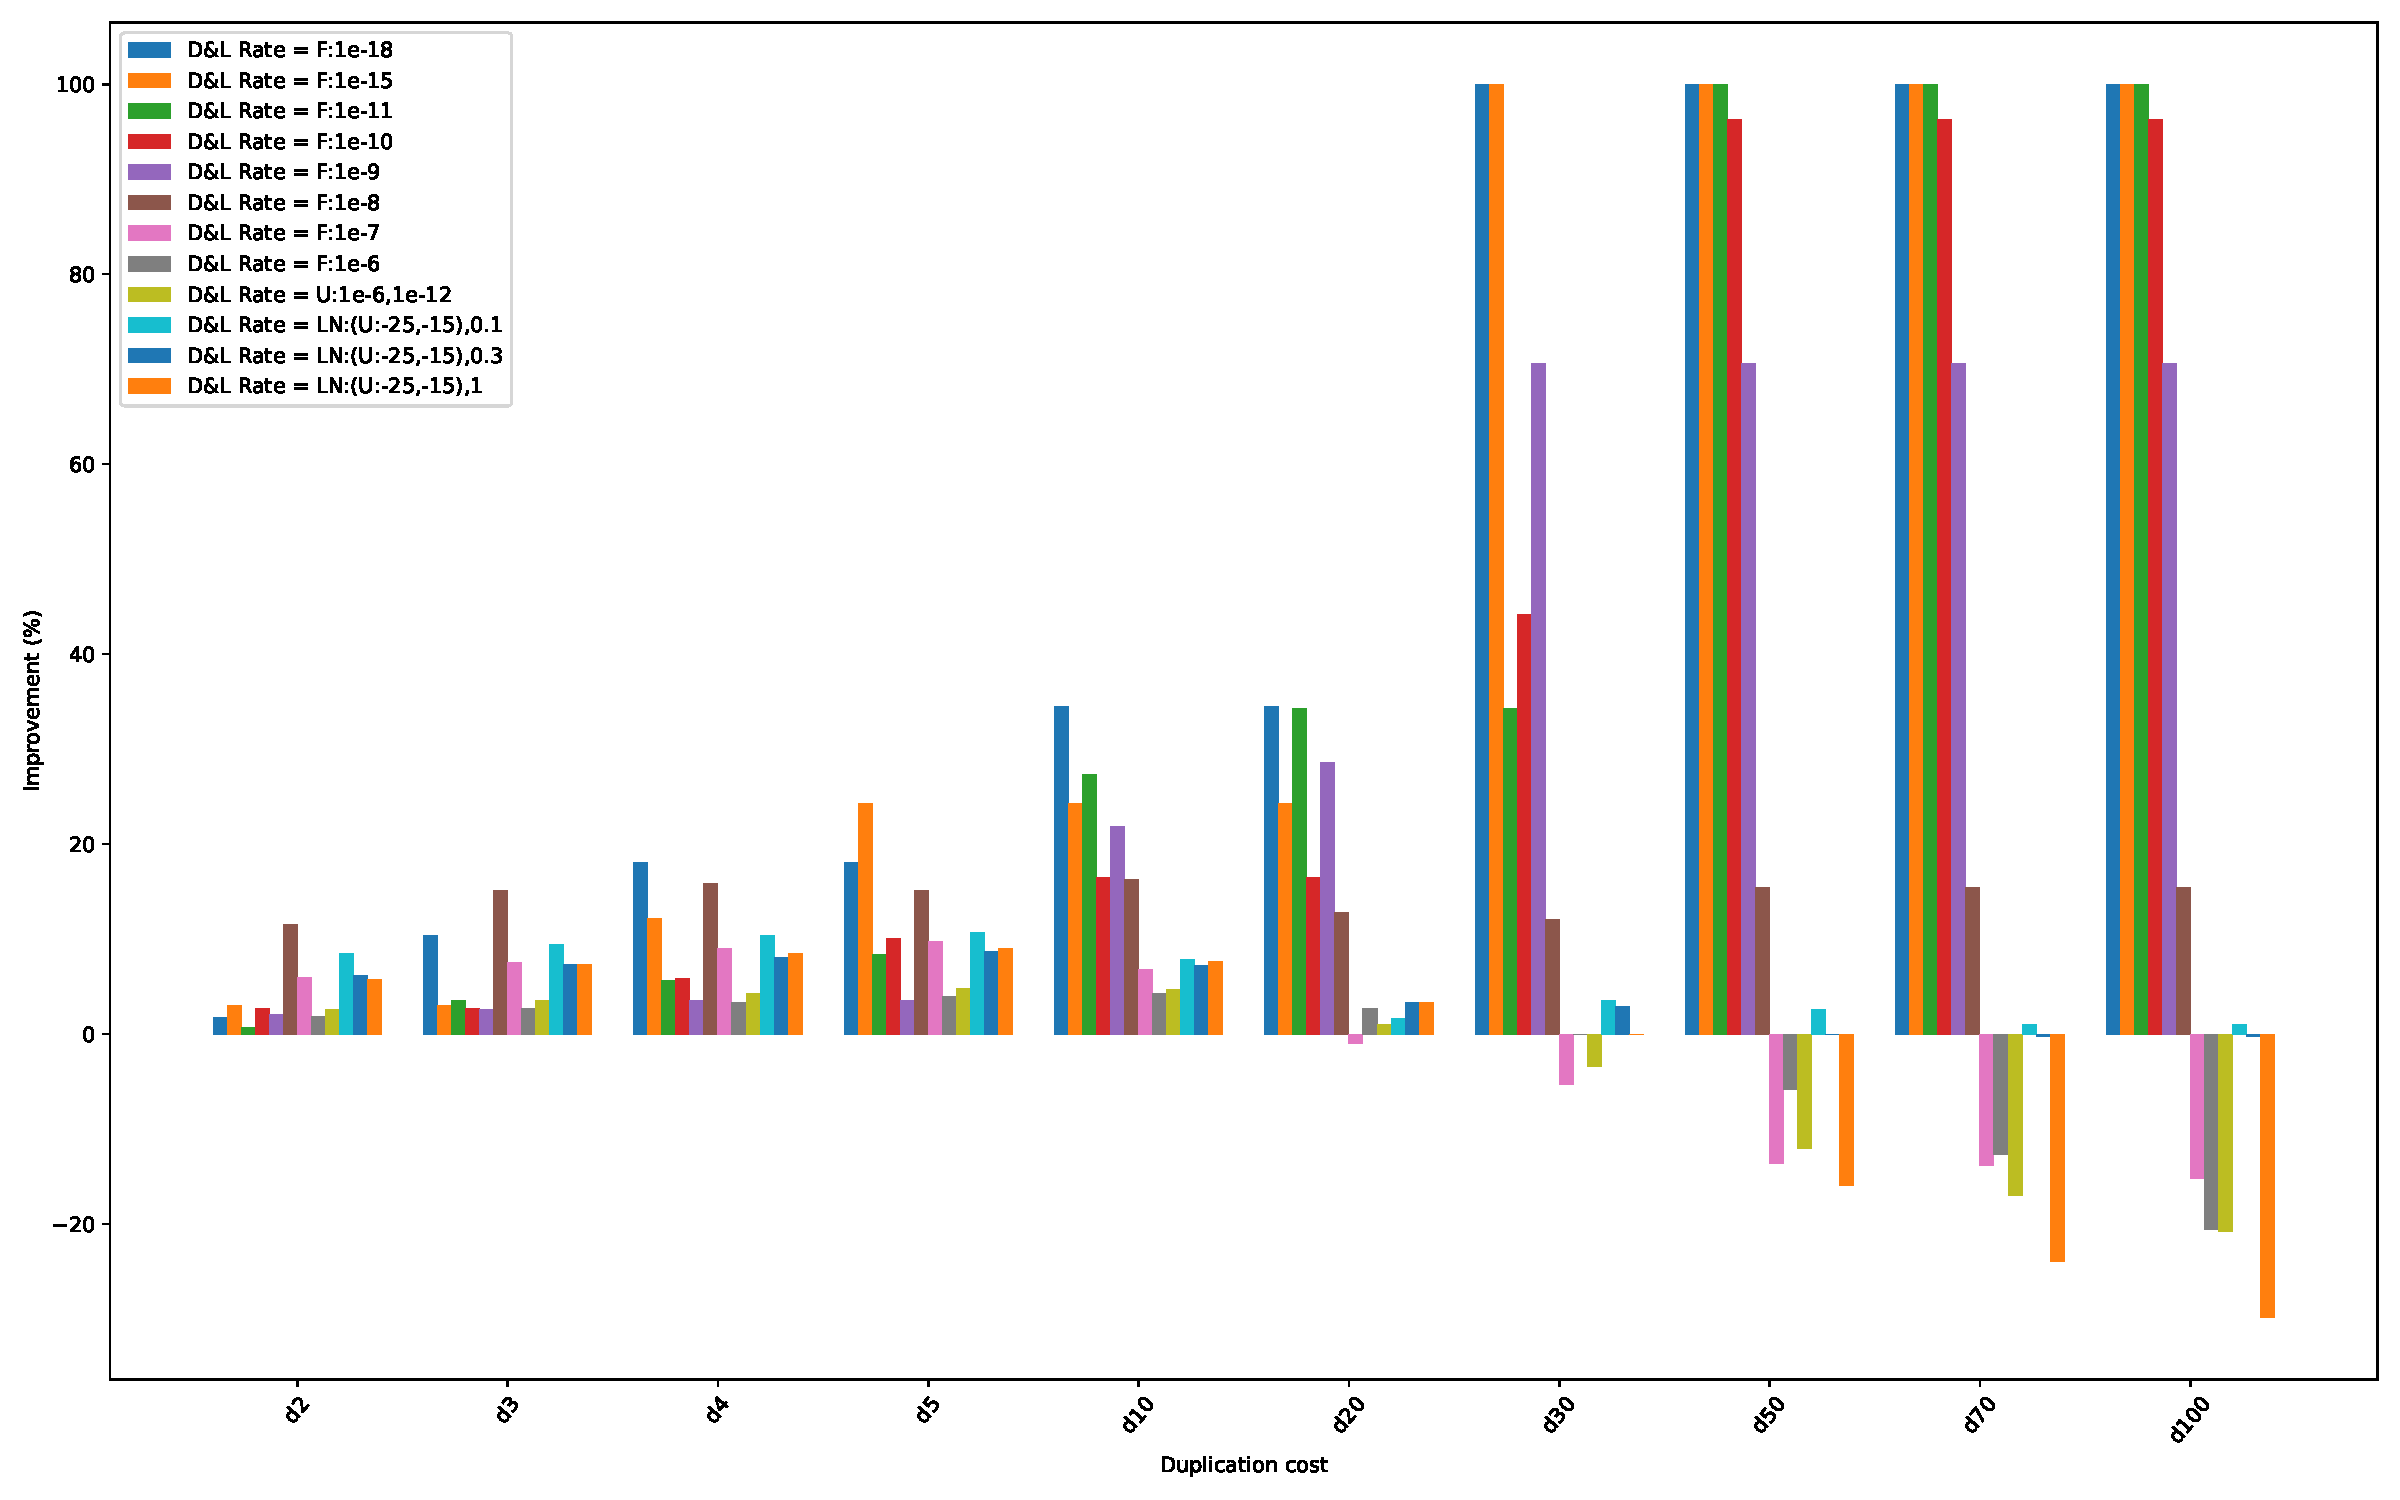
\includegraphics[width=1\textwidth]{figs/imp_1WGD.pdf}
    \caption{Improvement percentages for SimPhy simulations, each containing exactly one WGD events, where losses applied to the gene trees after the SimPhy simulation.}
    \label{fig:imp_1wgd_old}
\end{figure}

In Figure \ref{fig:imp_2wgd}, we present the improvement percentage results for SimPhy simulations where each simulation includes exactly two WGD events. The trends in this figure are similar to those in Figure \ref{fig:imp_1wgd}, which features simulations with a single WGD, showing similar effects of duplication and loss rates, as well as duplication cost. However, with two WGDs, the improvements tend to increase compared to Figure \ref{fig:imp_1wgd}. This is likely because the influence of random (non-tandem) duplications is reduced in our algorithm with a higher number of WGDs.

\begin{figure}[hbt!]
    \centering
    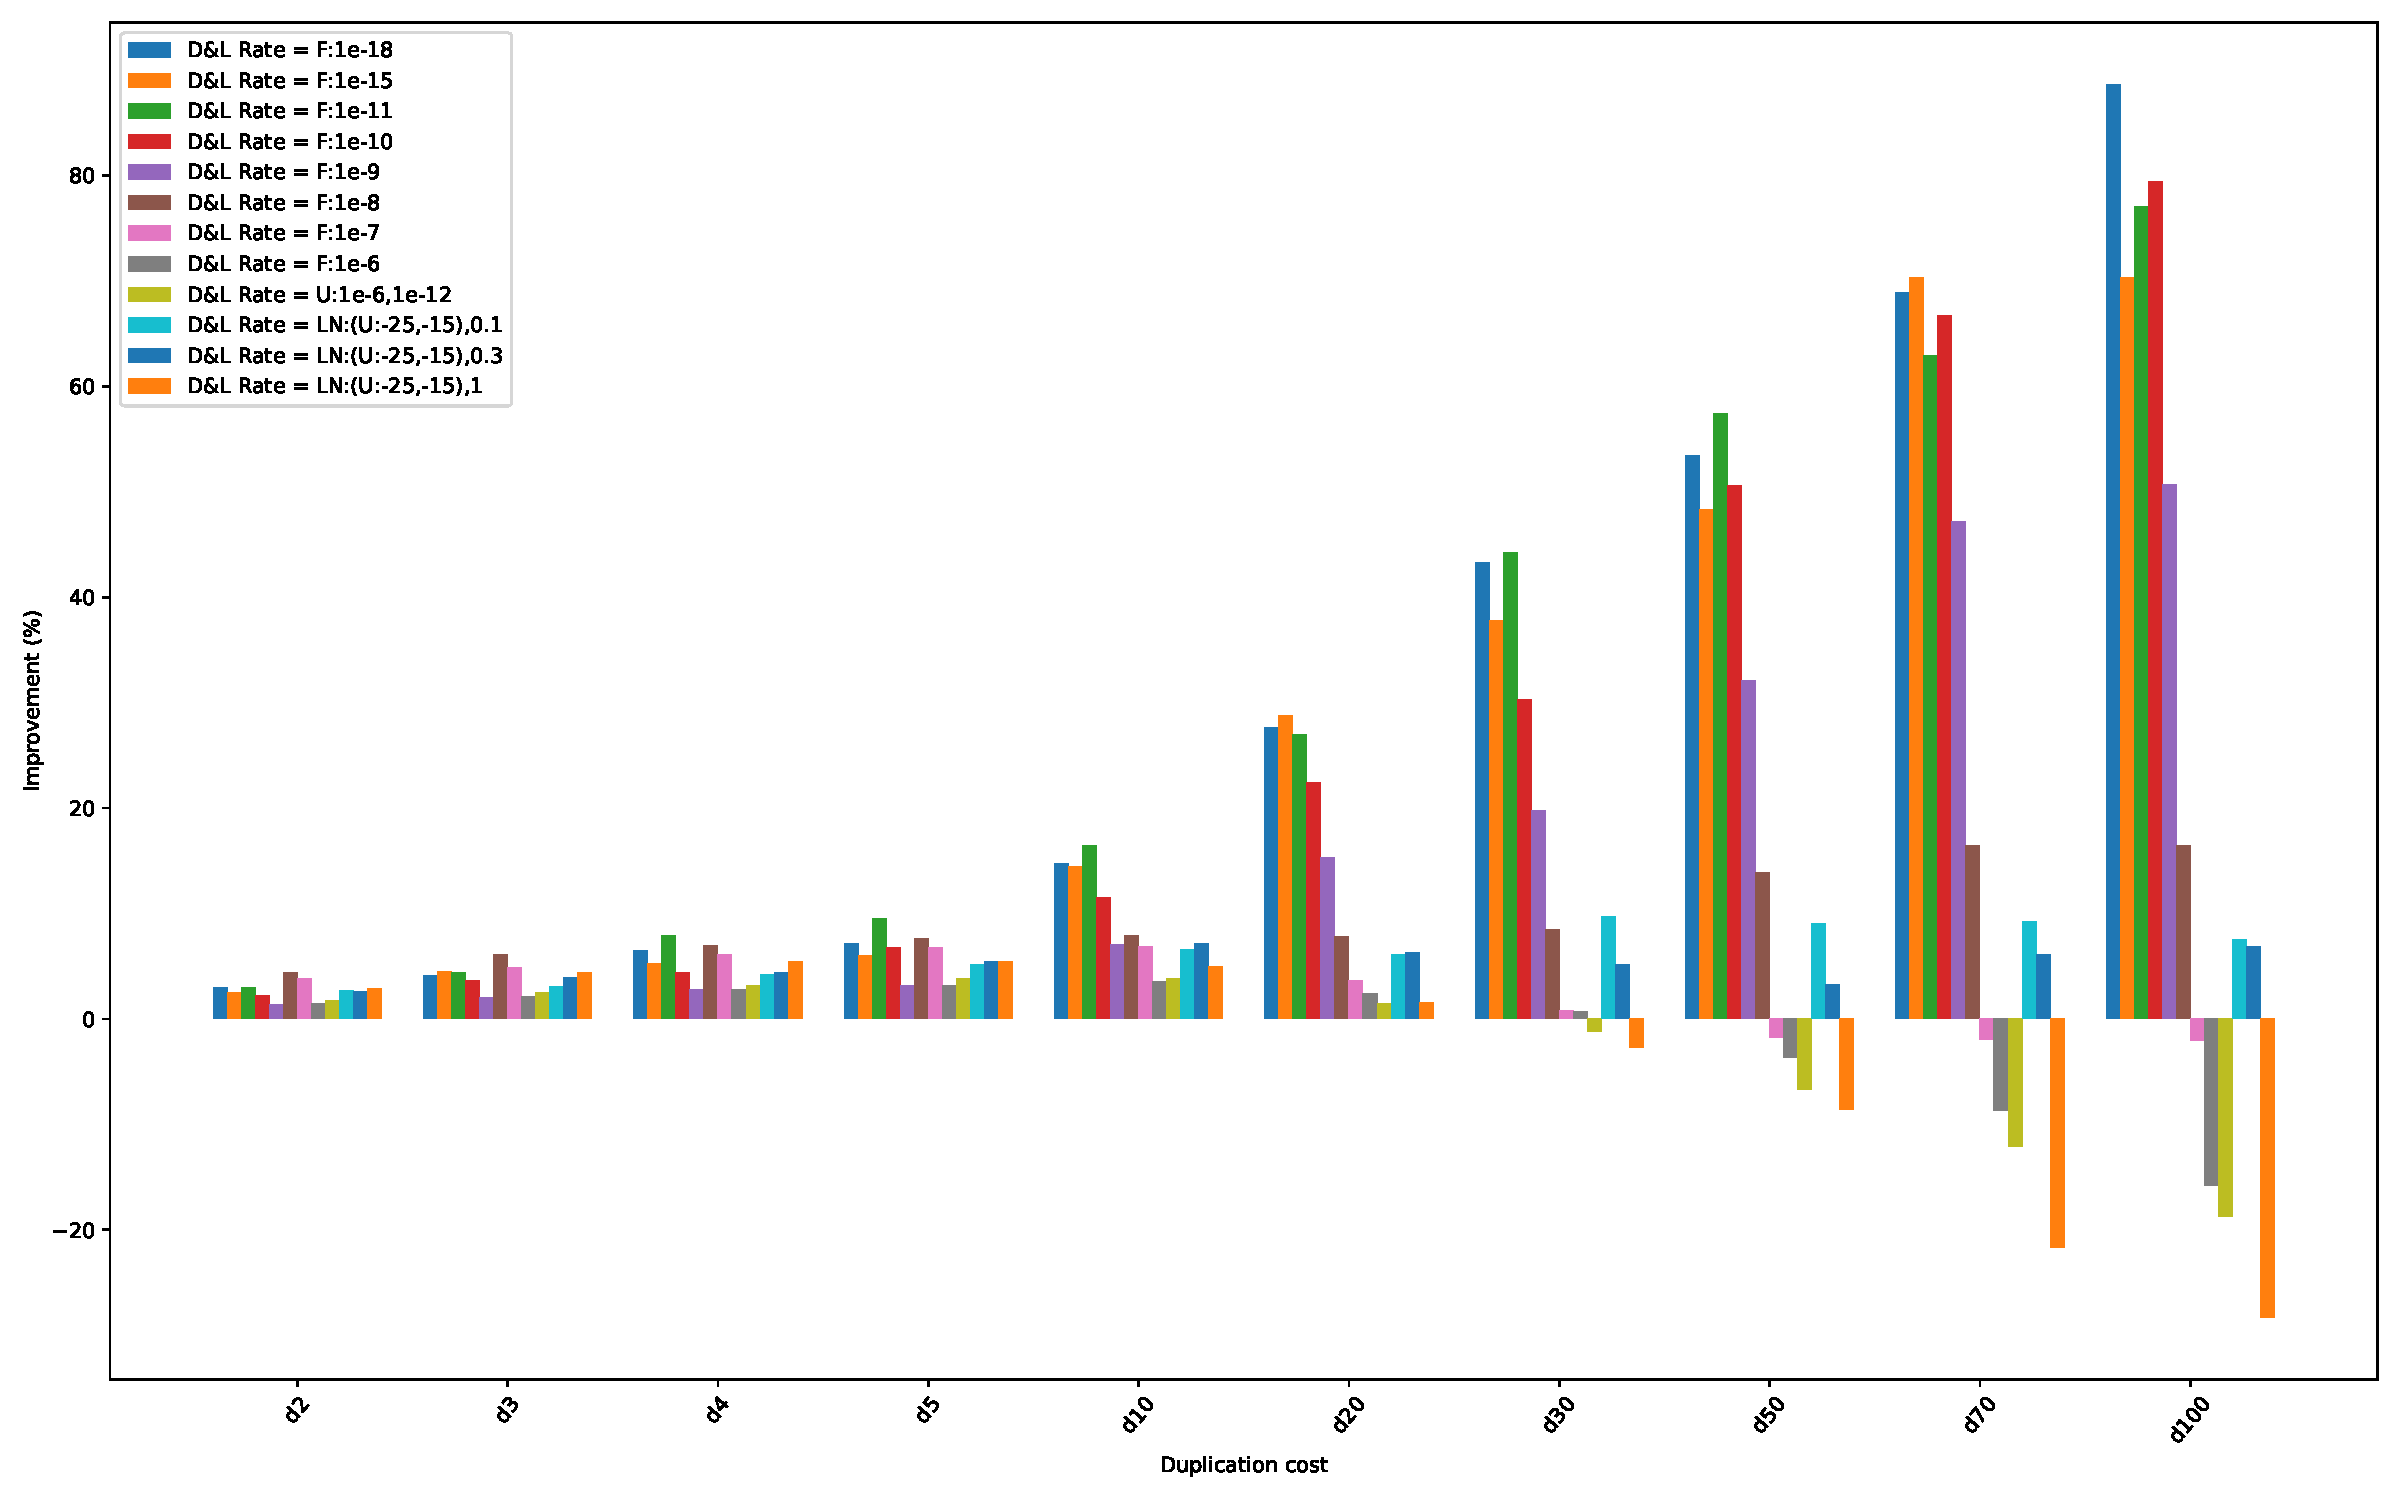
\includegraphics[width=1\textwidth]{figs/imp_2WGD.pdf}
    \caption{Improvement percentages for SimPhy simulations, each containing exactly two WGD events, where losses applied to the gene trees after the SimPhy simulation.}
    \label{fig:imp_2wgd}
\end{figure}

We also explored two additional versions of our algorithm. In the first variant, we disabled down moves (including bulk down moves), allowing only up moves to occur. This approach focuses on finding the best moves from the available up moves. The second variant, referred to as the stochastic version, calculates the total cost change for each possible move. It then uses a Boltzmann distribution to determine the probability of each move being selected like:

$$
\text{p}_i = \text{exp} \left(- \frac{\Delta C_i}{\text{T}}\right)
$$

where $\text{p}_i$ represents the probability of move $i$, $\Delta C_i$ denotes the total cost change associated with move $i$, and $\text{T}$ is the temperature parameter, set to 1. This probability formula allows us to weigh moves based on their cost changes, assigning higher probabilities to moves that result in greater reductions in total cost.

After computing the probabilities for all possible moves, we use a weighted random selection function to choose one move. This ensures that moves with higher probabilities are more likely to be selected. The stochastic algorithm performs this process for 2000 moves and returns the mapping that results in the lowest total cost out of these 2000 moves.

In Figure \ref{fig:imp_1wgd_allalg} and \ref{fig:imp_2wgd_allalg}, which present results for simulations with one and two WGDs, respectively, we compare the performance of three different versions of our algorithm, all using a duplication cost of 5. For scenarios with low duplication and loss rates, the version of our algorithm that disables down moves demonstrates superior performance. This improved performance can be attributed to the fact that with minimal losses, consistently mapping to higher species yields better results in terms of path distances. In these cases, avoiding down moves prevents unnecessary complexity and maintains more accurate mappings. However, for other duplication and loss rates, the three versions of the algorithm exhibit similar improvement percentages. This indicates that, under varying conditions, the advantage of disabling down moves may diminish, leading to comparable performance across the different algorithm versions.


\begin{figure}[hbt!]
    \centering
    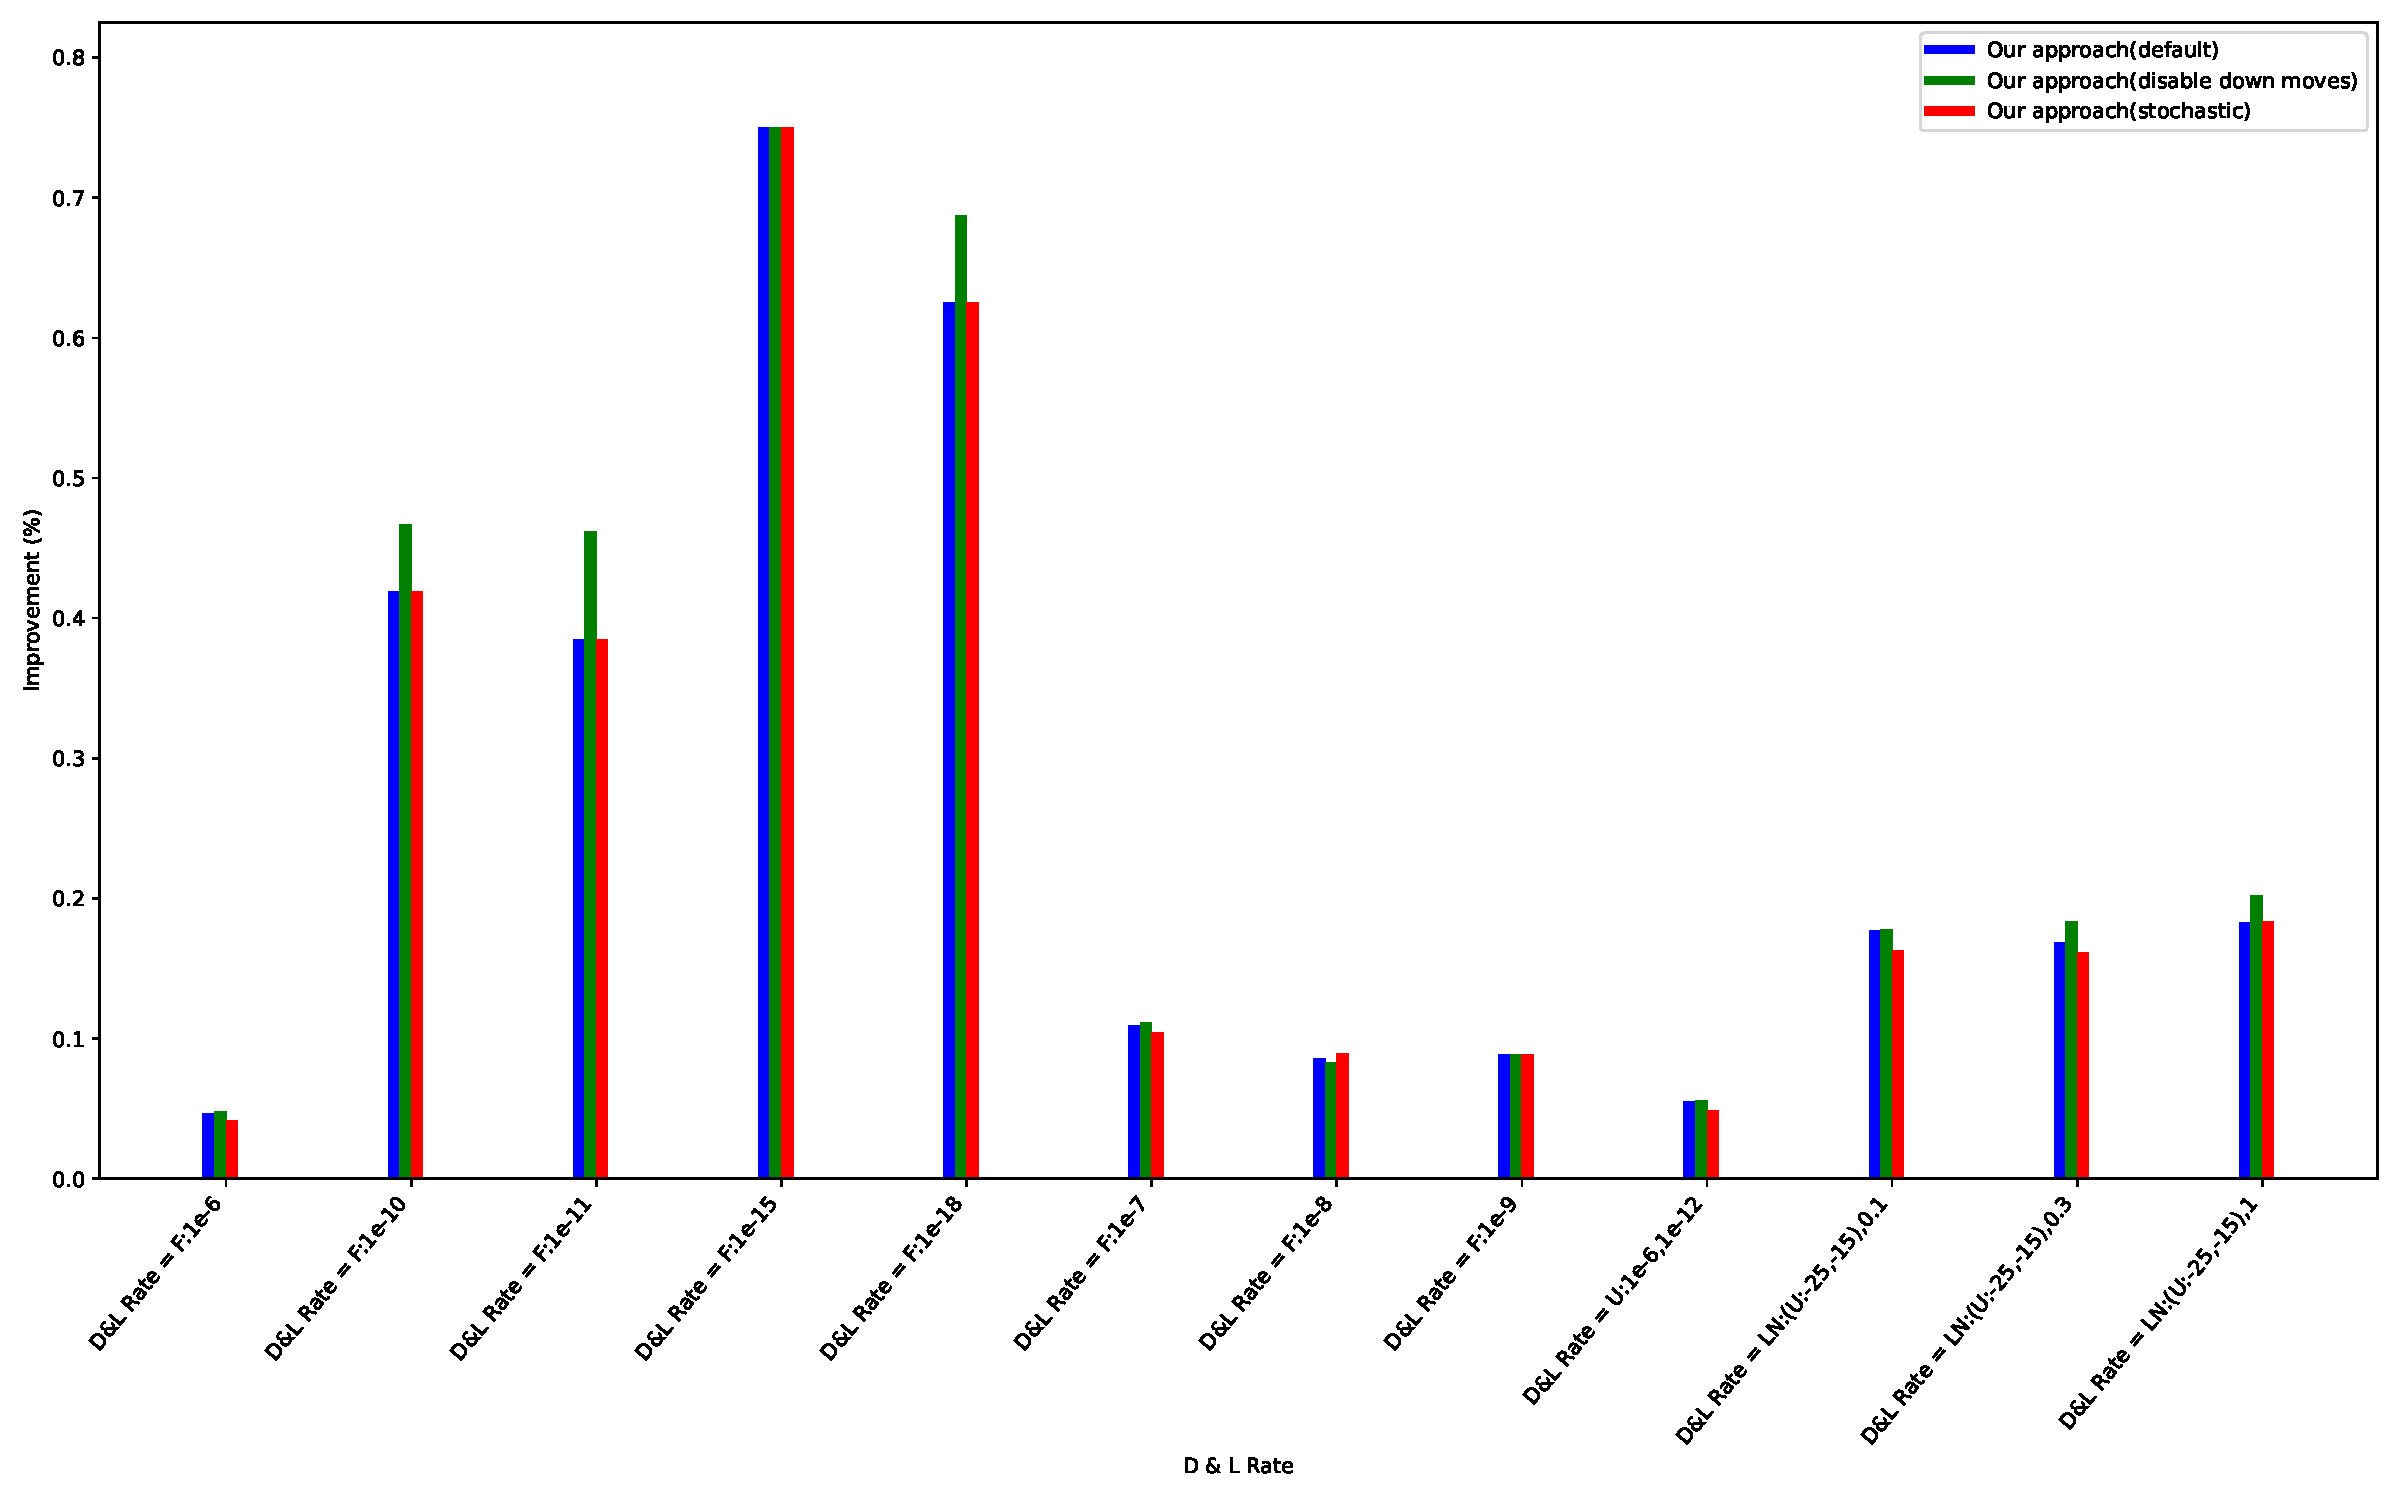
\includegraphics[width=1\textwidth]{figs_theory/imp_1WGD_allalgo_d5.pdf}
    \caption{Comparison of improvement percentages across three different versions of our algorithm for SimPhy simulations, each containing exactly one WGD events. In these simulations, losses were applied to the gene trees after the SimPhy simulation. This figure highlights how each algorithm version performs under varying conditions of duplication and loss rates.}
    \label{fig:imp_1wgd_allalg}
\end{figure}

\begin{figure}[hbt!]
    \centering
    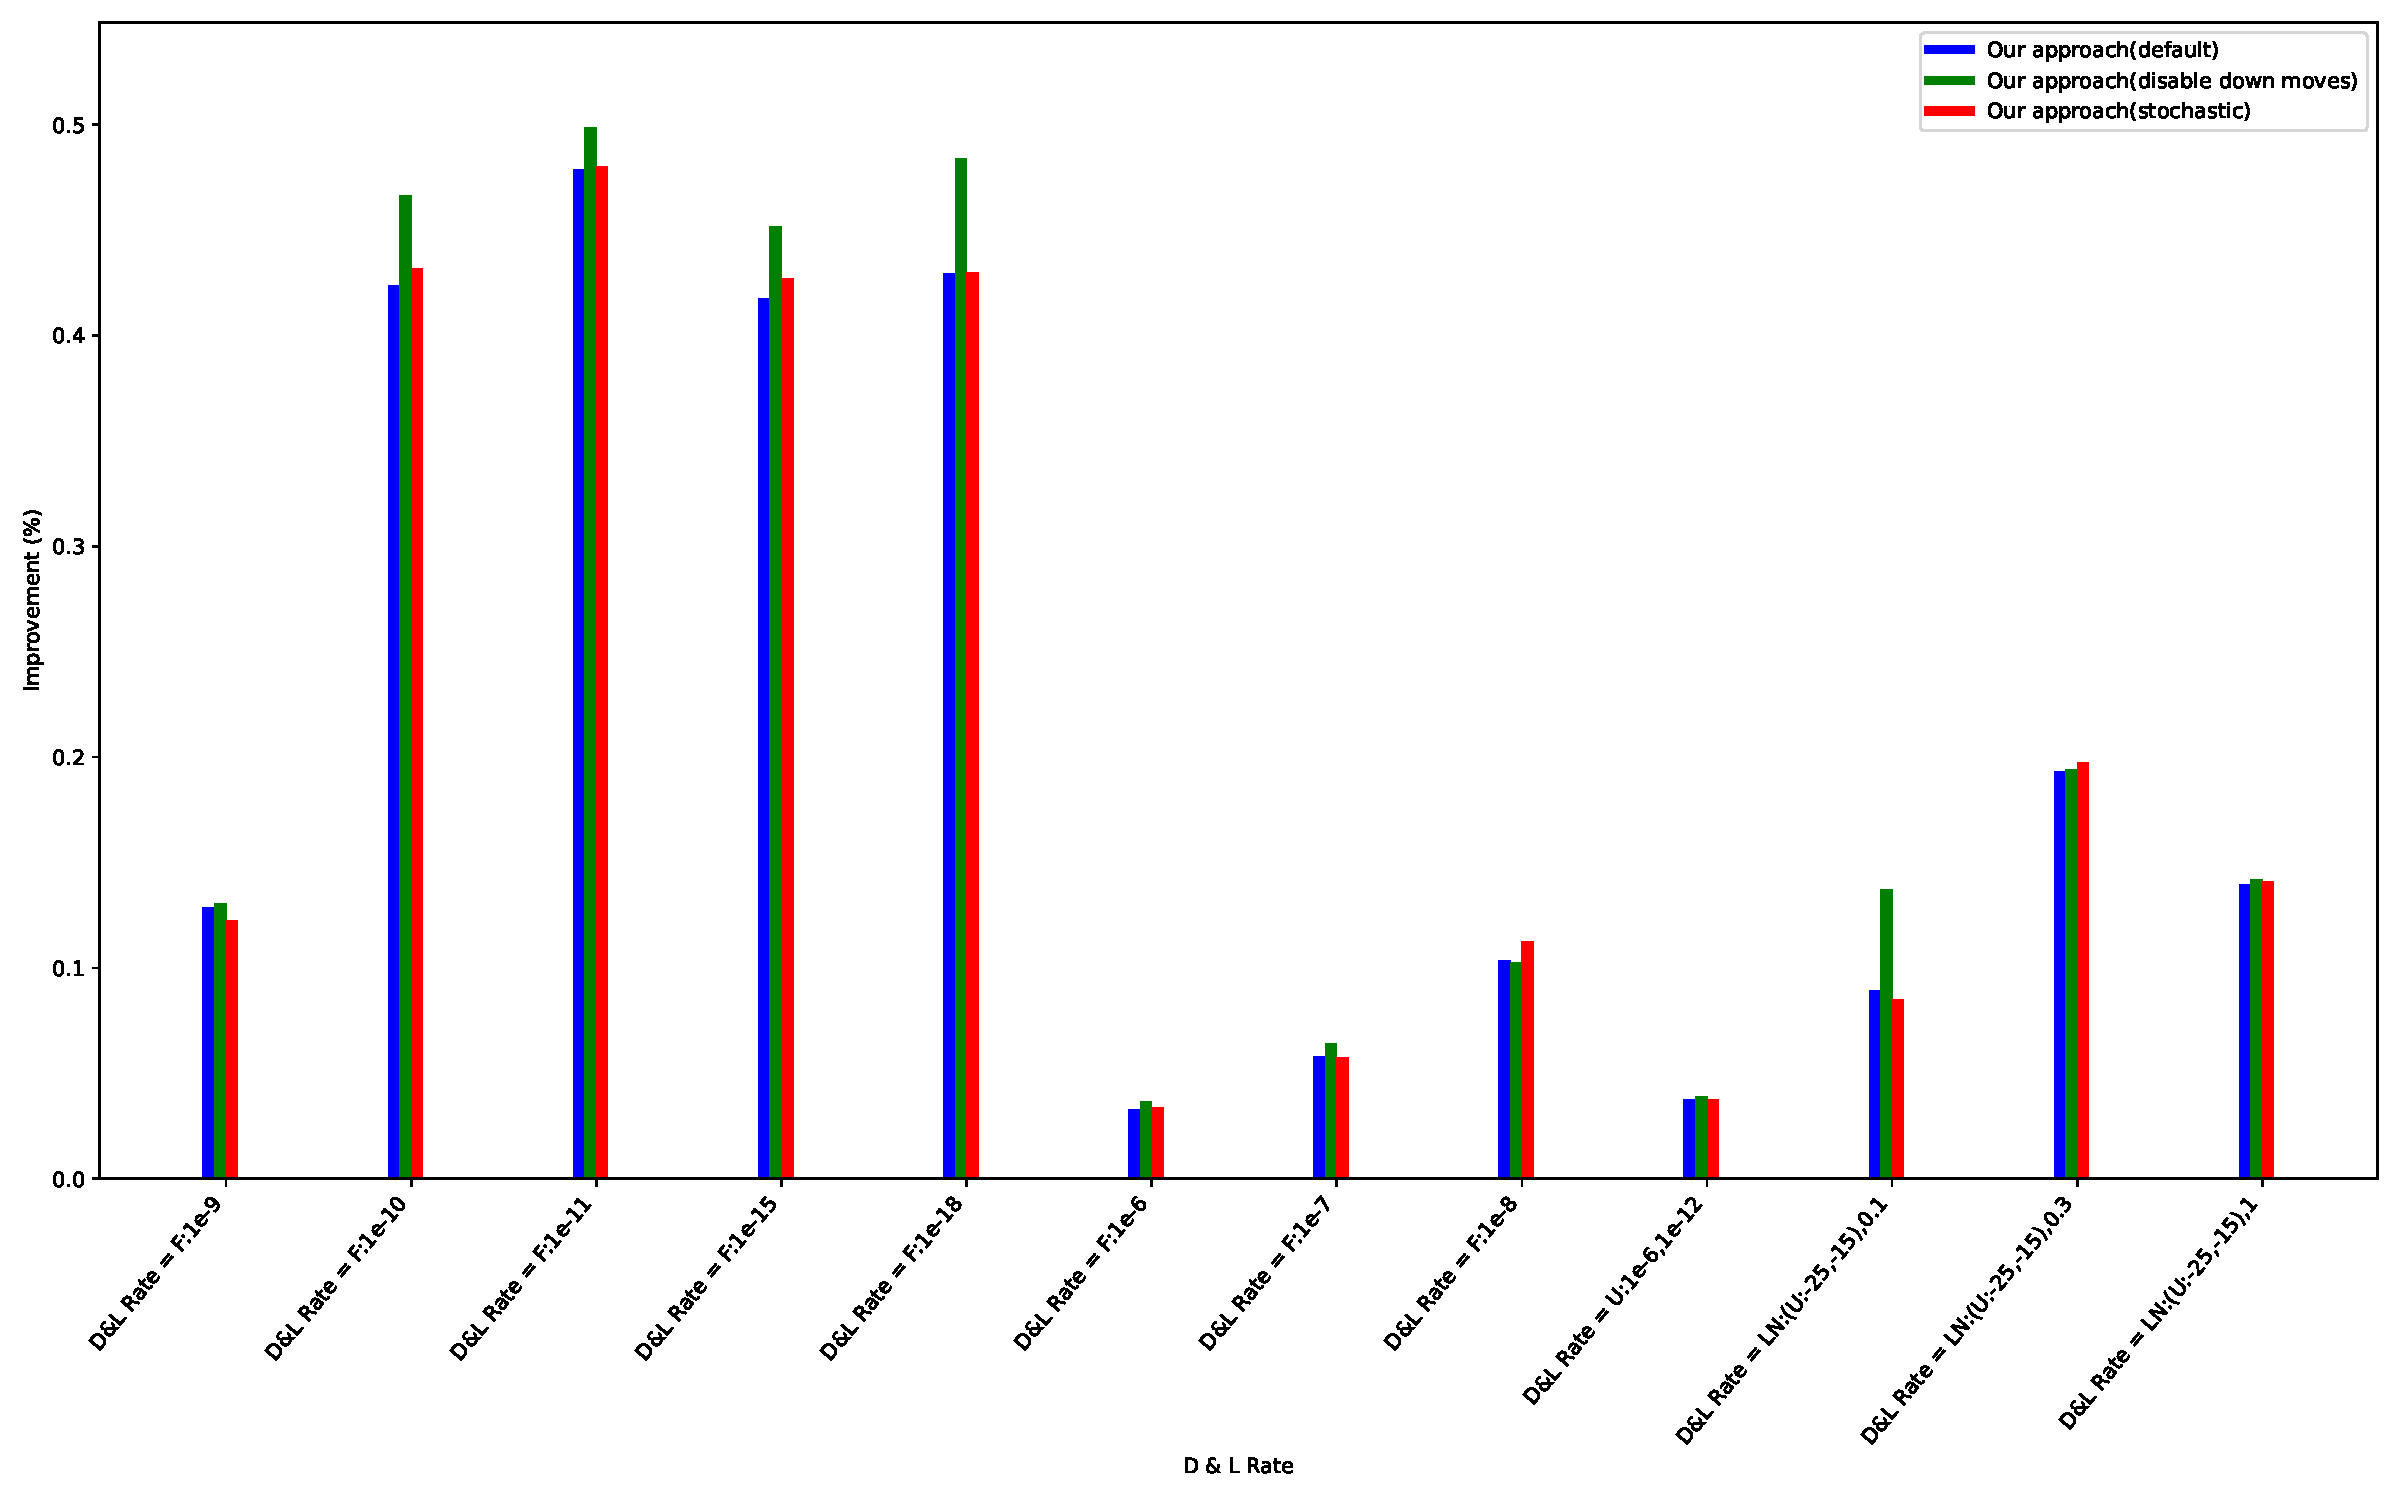
\includegraphics[width=1\textwidth]{figs_theory/imp_2WGD_allalgo_d5.pdf}
    \caption{Comparison of improvement percentages across three different versions of our algorithm for SimPhy simulations, each containing exactly two WGD events. In these simulations, losses were applied to the gene trees after the SimPhy simulation.}
    \label{fig:imp_2wgd_allalg}
\end{figure}


\subsection{Amplitudes}

The next metric we define is amplitude. For this metric, we examine each species across all gene trees, and the number of gene trees in which a species has a duplication is referred to as the number of $Gis$.

$$
\text{Amplitude(s)} = Gis(algorithm) - Gis(SimPhy)
$$

Here, $\text{Amplitude}(s)$ represents the amplitude value for species $s$, $Gis(\text{algorithm})$ is the number of gene trees in which species $s$ has a duplication according to the algorithm (either LCA or our approach), and $Gis(\text{SimPhy})$ represents the true number of $Gis$ for species $s$.


In Figure \ref{fig:amp}, we visualize the amplitude plot for species from a single simulation with a duplication and loss rate of $F:1e-11$. Subfigure \ref{fig:amp-a} shows the amplitude using the LCA mapping, while \ref{fig:amp-b} and \ref{fig:amp-c} display our approach with duplication costs of 5 and 100, respectively.

As observed in this simulation, there is only one WGD event. In the LCA mapping, the WGD is partially recovered, with some duplications being assigned to one of the descendants of the species (Note: the species on the x-axis are post-ordered).

Our approach with a duplication cost of 5 effectively reduces the noise present in the LCA mapping. When the duplication cost is increased to 100, our method fully recovers all duplications accurately, aligning perfectly with the true mapping. Notably, the Sum value is 0, indicating that the sum of all amplitudes for all species is zero, signifying no discrepancy between our approach and the true mapping.
 
\begin{figure}[h!]
    \centering
    % First subplot at the top
    \begin{subfigure}[b]{0.5\textwidth}
        \centering
        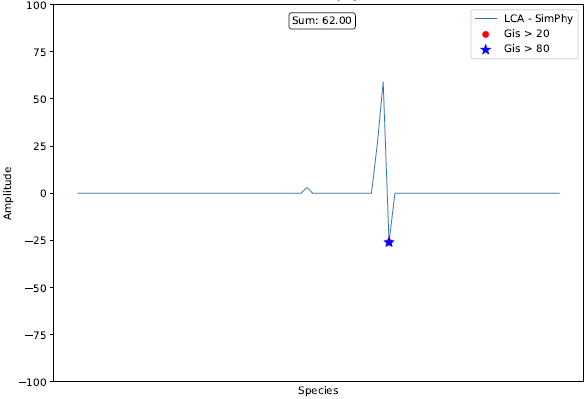
\includegraphics[width=\textwidth]{figs/LCA-amp.PNG}
        \caption{Amplitude plot for species using LCA mapping.}
        \label{fig:amp-a}
    \end{subfigure}
    
    % Two subplots in the second row
    \begin{subfigure}[b]{0.48\textwidth}
        \centering
        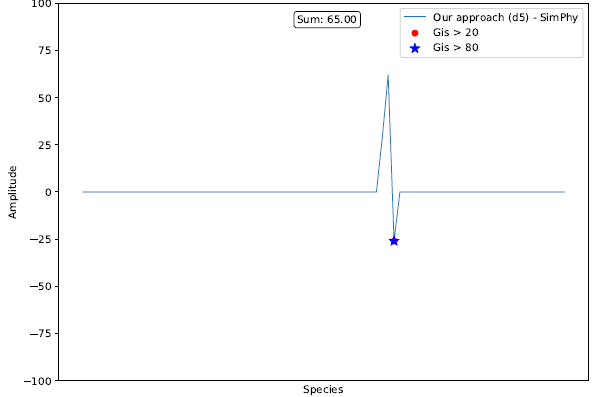
\includegraphics[width=\textwidth]{figs/greedy5-amp.PNG}
        \caption{Amplitude plot for species using our approach with duplication cost $d=5$.}
        \label{fig:amp-b}
    \end{subfigure}
    \hfill
    \begin{subfigure}[b]{0.48\textwidth}
        \centering
        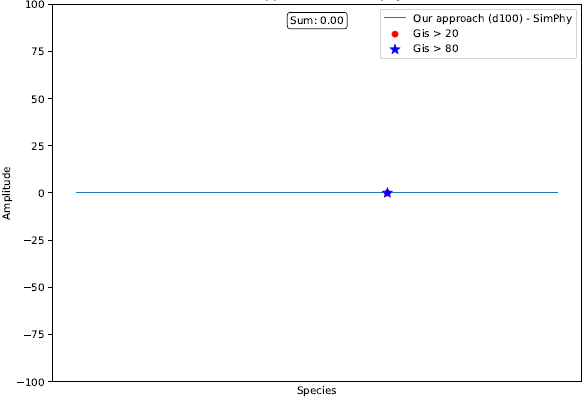
\includegraphics[width=\textwidth]{figs/greedy100-amp.PNG}
        \caption{Amplitude plot for species using our approach with duplication cost $d=100$.}
        \label{fig:amp-c}
    \end{subfigure}
    
    \caption{
    Amplitude plots from a single simulation with duplication and loss rates set to $F:1e-11$. These plots illustrate the differences in the number of duplications across gene trees for each species. We apply thresholds to classify duplication events as either whole genome duplications (WGD) or segment duplications (SD). Specifically, a species with duplications in more than 80\% of gene trees is classified as experiencing a WGD, indicated by a blue star in the figure. Conversely, a species with duplications in more than 20\% but less than 80\% of gene trees is classified as an SD, indicated by a red circle. The Sum value in each plot represents the sum of all y-values, where a positive number indicates that the algorithm identified more duplications than the true number, and a negative number indicates fewer. Therefore, the closer the Sum value is to 0, the more accurate the algorithm is in detecting duplications. This visualization helps to compare the performance of LCA mapping against our approach under different duplication cost settings.
    }
    \label{fig:amp}
\end{figure}





\subsection{Recall and Precision}
In this section, we define Recall and Precision for our approach. To do so, we first need to establish the concepts of True Positives, False Negatives, and False Positives. Additionally, before introducing these measures, it is essential to clarify how we define Whole Genome Duplication (WGD) and Segmental Duplication (SD) within our simulations.

\textbf{Whole Genome Duplication (WGD):} A species is considered to have undergone a WGD if it exhibits duplication in more than 80\% of the gene trees.

\textbf{Segmental Duplication (SD):} A species is considered to have undergone SD if it shows duplication in more than 20\% but less than 80\% of the gene trees.

\textbf{True Positives (TP):} A species is counted as a true positive if it has a WGD in the true simulation and is also identified as having a WGD in our approach or LCA.

\textbf{False Negatives (FN):} A species is counted as a false negative if it has a WGD in the true simulation but is not identified as having a WGD in our approach or LCA.

\textbf{False Positives (FP):} A species is counted as a false positive if it does not have a WGD in the true simulation but is incorrectly identified as having a WGD in our approach or LCA.

The same definitions apply when evaluating SD events.

\textbf{Recall}, also known as sensitivity or true positive rate, is a metric that quantifies the ability of our approach to correctly identify positive instances out of all the actual positive cases. It reflects the completeness of the positive predictions. A high recall indicates that the method successfully captures most of the true positive events, minimizing the number of false negatives.

$$
\text{Recall} = \frac{\text{TP}}{\text{TP+FN}}
$$

\textbf{Precision} measures the accuracy of the positive predictions made by the approach. It is the proportion of true positive cases among all cases predicted as positive. Precision reflects the reliability of the positive predictions, indicating how often the positive predictions are actually correct. A high precision means that when the method predicts a positive case, it is likely to be correct, reducing the occurrence of false positives.

$$
\text{Precision} = \frac{\text{TP}}{\text{TP+FP}}
$$

Finally, since all these metrics—Recall, Precision, and others—are calculated for a single simulation, and we have 100 repeated simulations for each duplication and loss rate in SimPhy, we take the average of these metrics across all 100 simulations for each specific duplication and loss rate. This averaging process allows us to obtain a more robust and reliable estimate of the algorithm's performance, and we can better understand how our approach performs under different conditions and gain insights into the overall trends across varying duplication and loss rates.

\begin{figure}[h!]
    \centering
    % First subplot at the top
    \begin{subfigure}[b]{0.48\textwidth}
        \centering
        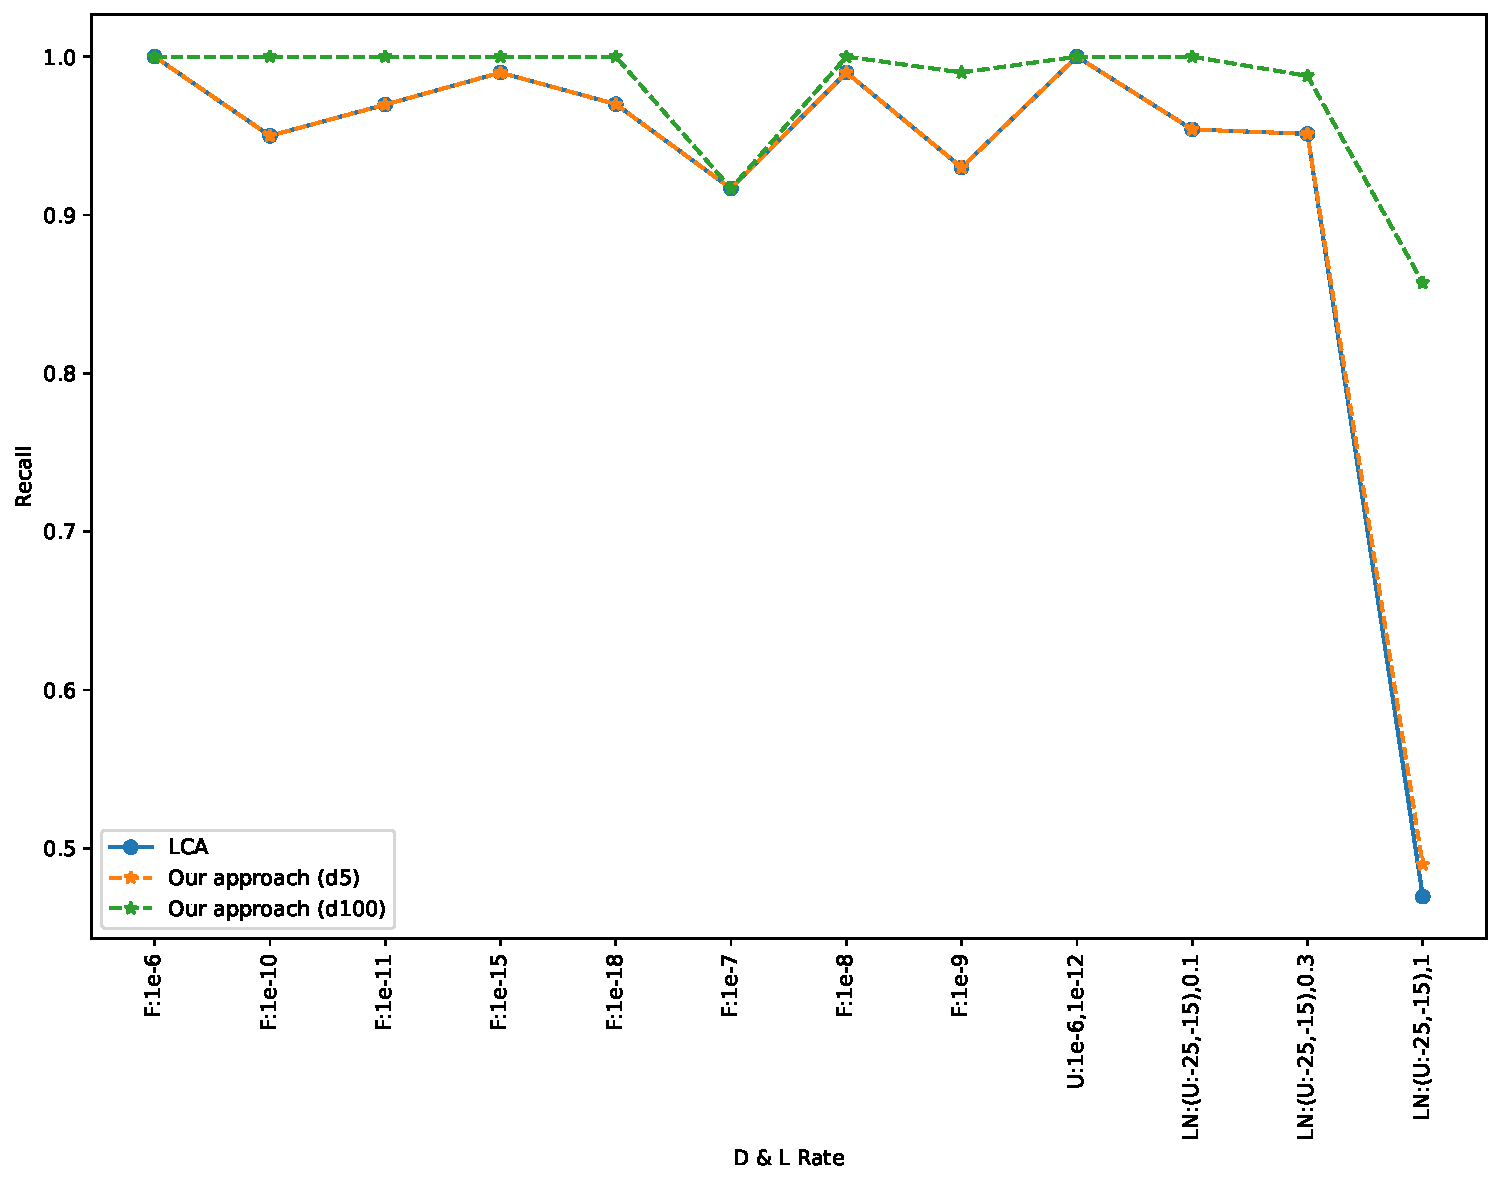
\includegraphics[width=\textwidth]{figs/recall-WGD-t10-t80-Avg.pdf}
        \caption{Recall of WGD for simulations with 1 WGD, averaged over 100 runs.}
        \label{fig:recall-wgd-1wgd_old}
    \end{subfigure}
    \hfill
    \begin{subfigure}[b]{0.48\textwidth}
        \centering
        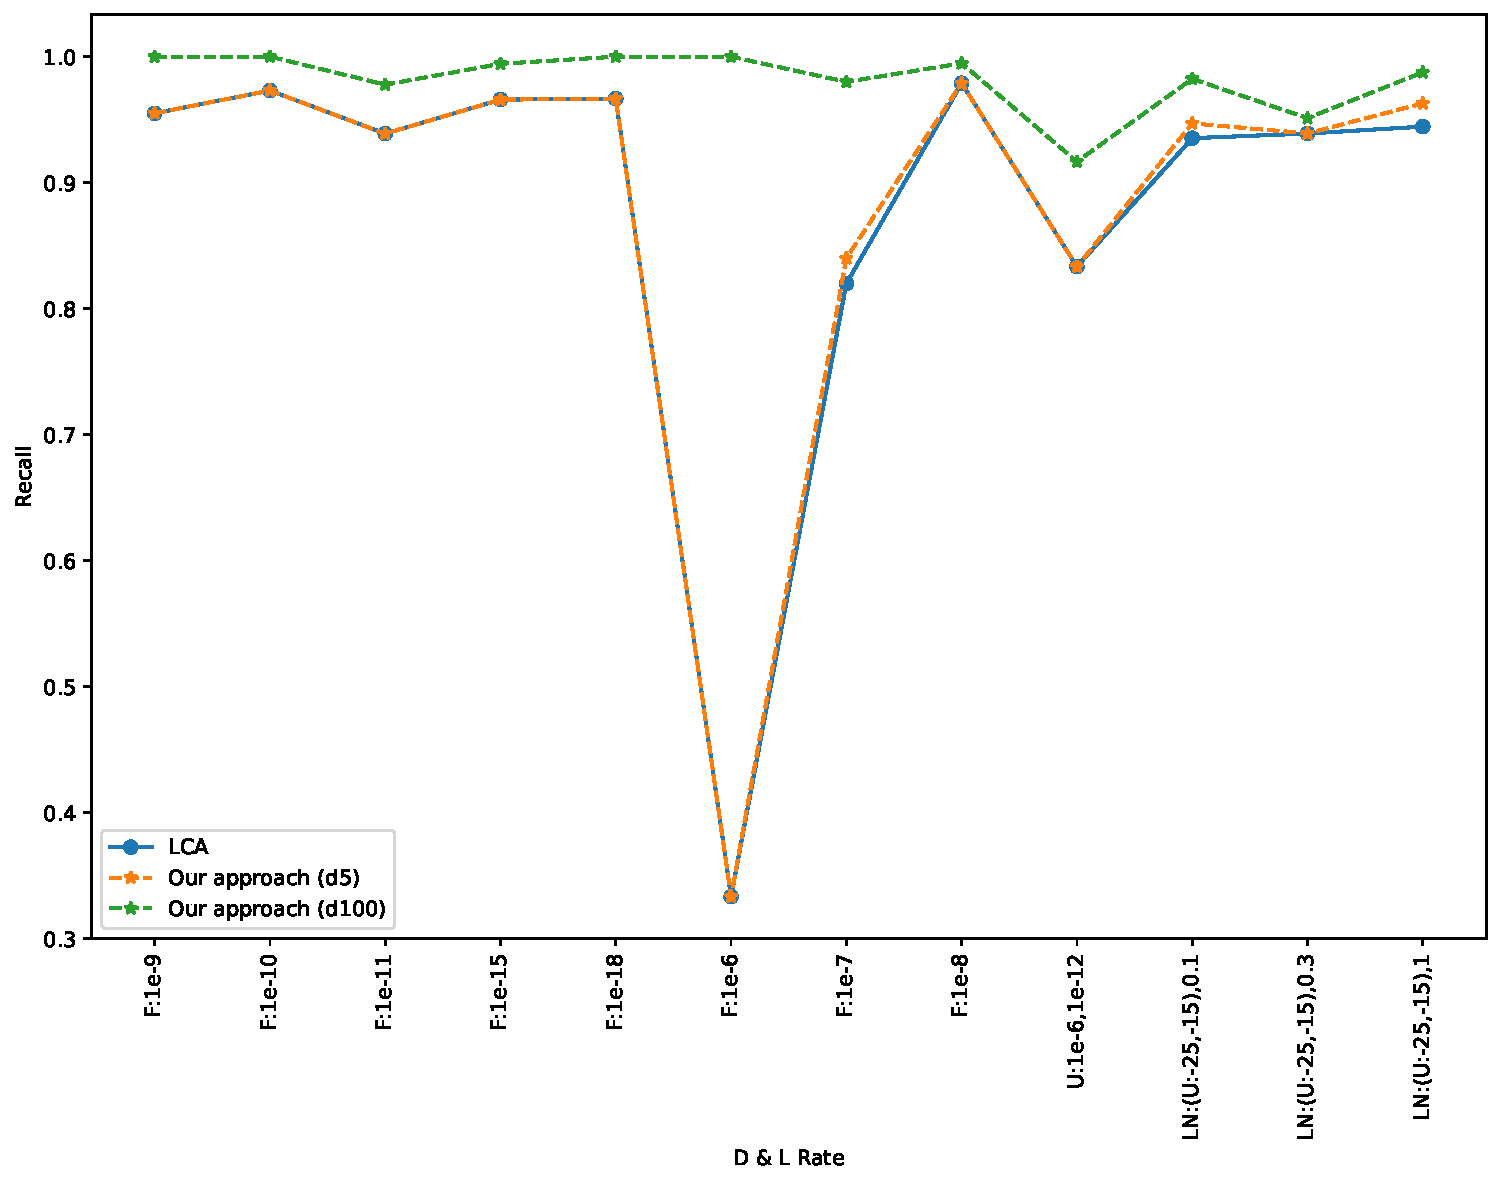
\includegraphics[width=\textwidth]{figs/recall-2W-WGD-t20-t80-Avg.pdf}
        \caption{Recall of WGD for simulations with 2 WGDs, averaged over 100 runs.}
        \label{fig:recall-wgd-2wgd}
    \end{subfigure}
    
    % Two subplots in the second row
    \begin{subfigure}[b]{0.48\textwidth}
        \centering
        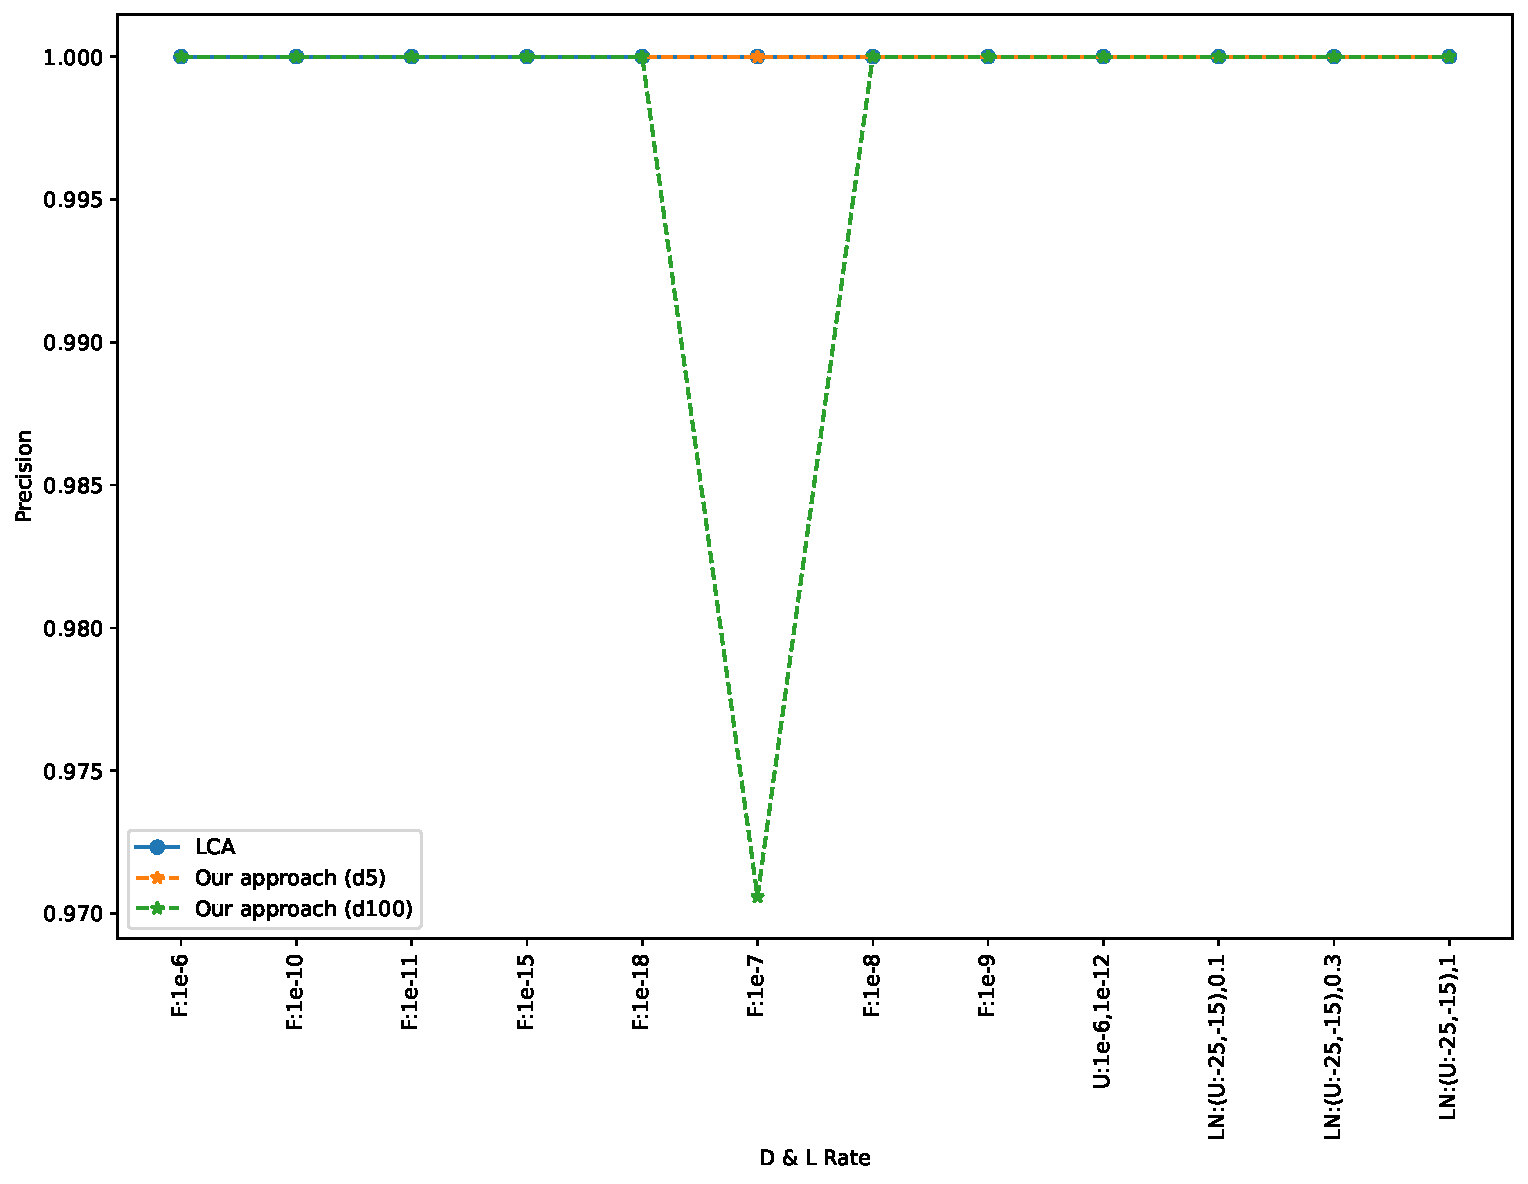
\includegraphics[width=\textwidth]{figs/precision-WGD-t10-t80-Avg.pdf}
        \caption{Precision of WGD for simulations with 1 WGD, averaged over 100 runs.}
        \label{fig:precision-wgd-1wgd_old}
    \end{subfigure}
    \hfill
    \begin{subfigure}[b]{0.48\textwidth}
        \centering
        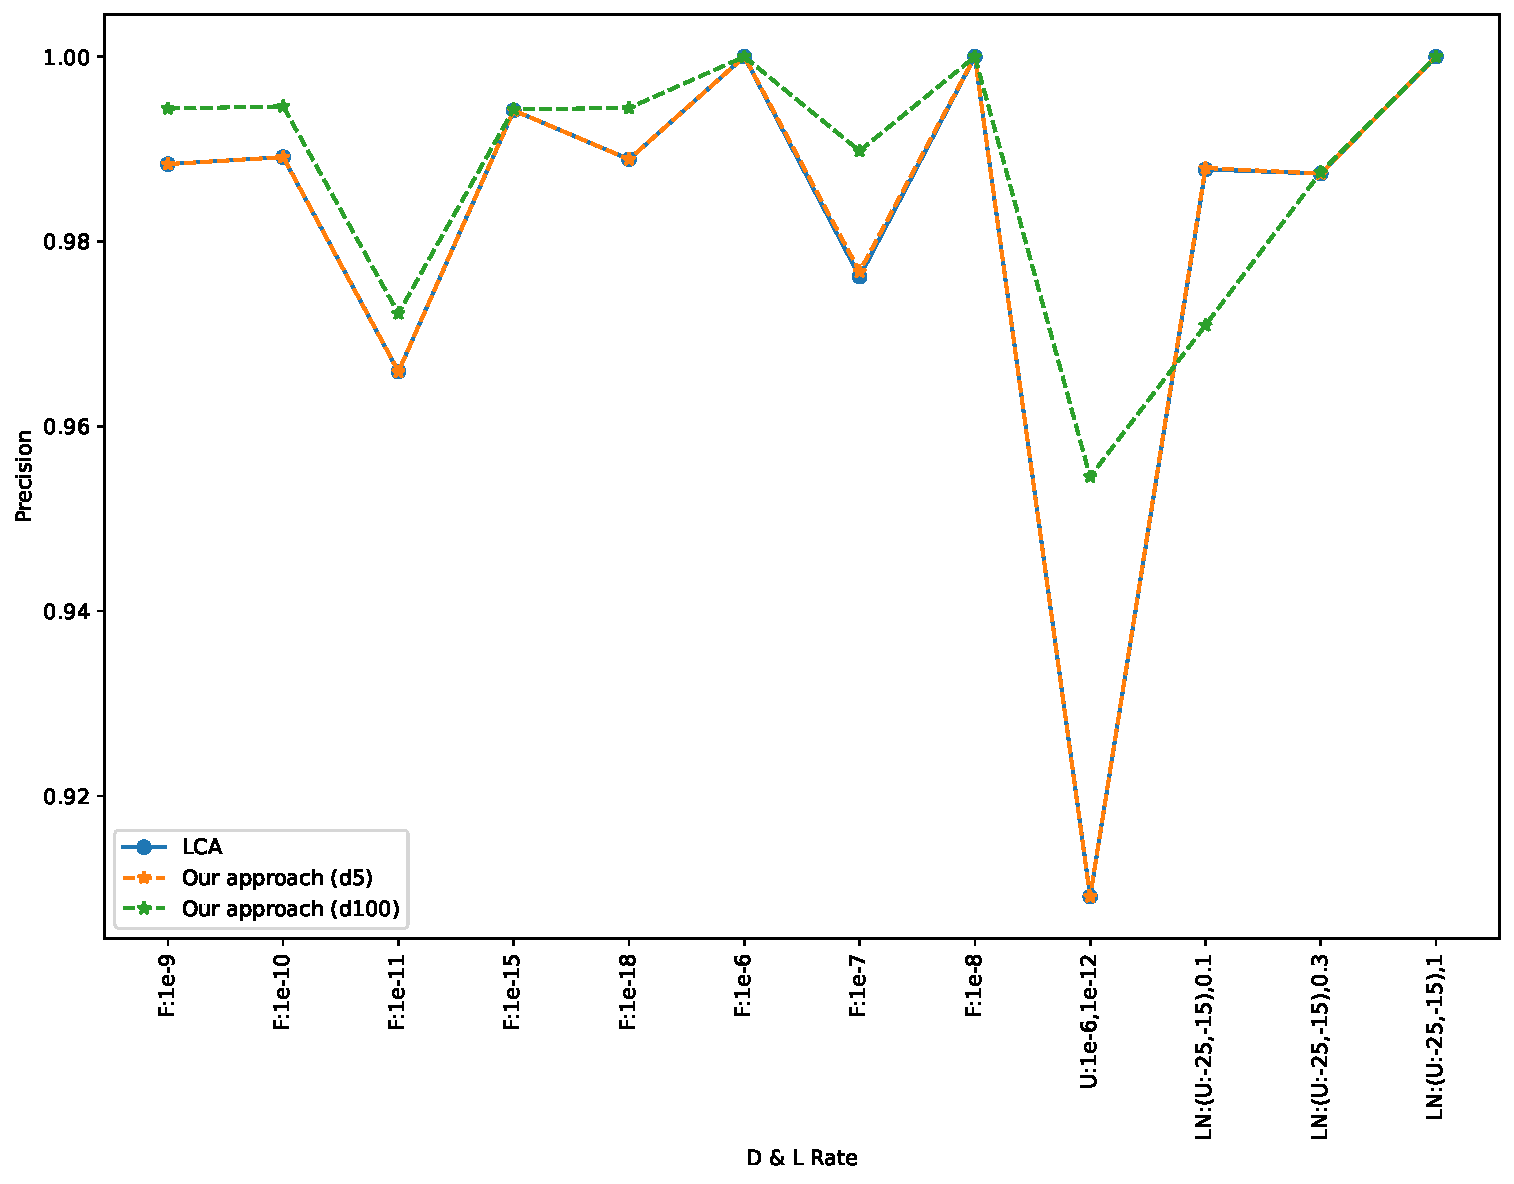
\includegraphics[width=\textwidth]{figs/precision-2W-WGD-t20-t80-Avg.pdf}
        \caption{Precision of WGD for simulations with 2 WGDs, averaged over 100 runs.}
        \label{fig:precision-wgd-2wgd}
    \end{subfigure}
    
    \caption{
Recall and Precision metrics for detecting Whole Genome Duplication (WGD) events in simulations containing either one or two WGDs, analyzed under varying duplication and loss rates. Each result is an average derived from 100 simulation runs, ensuring reliability and robustness of the findings. Subfigure (a) shows the Recall metric for simulations with a single WGD, while subfigure (b) presents the Recall for simulations with two WGDs. Subfigures (c) and (d) display the Precision metrics for simulations with one and two WGDs, respectively.
    }
    \label{fig:recall-precision-wgd_old}
\end{figure}





\begin{figure}[h!]
    \centering
    % First subplot at the top
    \begin{subfigure}[b]{0.48\textwidth}
        \centering
        \includegraphics[width=\textwidth]{figs/recall-sd-t20-t80-Avg.pdf}
        \caption{Recall of SD for simulations with 1 WGD, averaged over 100 runs.}
        \label{fig:recall-sd-1wgd}
    \end{subfigure}
    \hfill
    \begin{subfigure}[b]{0.48\textwidth}
        \centering
        \includegraphics[width=\textwidth]{figs/recall-2W-sd-t20-t80-Avg.pdf}
        \caption{Recall of SD for simulations with 2 WGDs, averaged over 100 runs.}
        \label{fig:recall-sd-2wgd}
    \end{subfigure}
    
    % Two subplots in the second row
    \begin{subfigure}[b]{0.48\textwidth}
        \centering
        \includegraphics[width=\textwidth]{figs/precision-sd-t20-t80-Avg.pdf}
        \caption{Precision of SD for simulations with 1 WGD, averaged over 100 runs.}
        \label{fig:precision-sd-1wgd}
    \end{subfigure}
    \hfill
    \begin{subfigure}[b]{0.48\textwidth}
        \centering
        \includegraphics[width=\textwidth]{figs/precision-2W-sd-t20-t80-Avg.pdf}
        \caption{Precision of SD for simulations with 2 WGDs, averaged over 100 runs.}
        \label{fig:precision-sd-2wgd}
    \end{subfigure}
    
    \caption{
        Recall and Precision metrics for predicting Segmental Duplications (SDs) in simulations featuring either one or two Whole Genome Duplications (WGDs), evaluated under different duplication and loss rates. Each metric is averaged over 100 simulation runs to ensure robust statistical significance. Subfigures (a) and (b) display the Recall for simulations with 1 and 2 WGDs, respectively, while subfigures (c) and (d) present the corresponding Precision metrics. These plots provide insights into the algorithm's ability to accurately predict SDs under varying evolutionary scenarios.
    }
    \label{fig:recall-precision-sd}
\end{figure}


\subsection{Results under Nearest Neighbor Interchanges (NNI) Event}

In this section, we analyze the performance of our approach when Nearest Neighbor Interchanges (NNI) events are introduced into the gene trees. NNI is a tree rearrangement method that swaps the subtrees around an internal node, effectively altering the tree topology without changing the leaf labels. By applying NNIs, we simulate more complex evolutionary scenarios that challenge the accuracy of ancestral mapping.

We conducted a series of experiments where NNI events were applied to the gene trees after simulating duplications and losses with SimPhy. These tests allow us to evaluate the robustness of our algorithm in dealing with uncertainties introduced by such topological changes. Specifically, we analyze how the introduction of NNI events impacts the recall and precision metrics for WGDs and SDs in both one and two WGD simulations.

We define a value $k$ in NNI, representing the number of Nearest Neighbor Interchanges applied to each gene tree. To assess the impact of varying degrees of tree rearrangement, we tested three different values of $k$: a low NNI rate ($k=1$), a medium NNI rate ($k=5$), and a high NNI rate ($k=15$). These values correspond to increasing levels of topological alteration in the gene trees, simulating various degrees of evolutionary complexity.

In Figures \ref{fig:recall-precision-wgd-NNI} and \ref{fig:recall-precision-2wgd-NNI}, we present the recall and precision metrics for simulations containing one and two WGDs, respectively. In terms of recall, we observe that across all NNI rates, our approach consistently outperforms the LCA method, particularly when two WGD events are present. This suggests that even under significant gene tree rearrangements, our method is better at recovering true WGD events compared to the LCA-based mapping.

However, in terms of precision, we note that for scenarios with high duplication and loss rates, our approach exhibits a lower precision rate, particularly as the NNI rate increases. This indicates that, while our method successfully identifies many true positives, it also introduces more false positives under high NNI and complex duplication scenarios. This trend is more pronounced in simulations with higher duplication rates and complex topological rearrangements, where over-estimating WGD events may become an issue.

These results highlight the robustness of our approach in recovering WGD events under varying levels of tree rearrangement, while also pointing out potential areas for improvement in precision, particularly under high duplication rates and extensive tree modifications.



\begin{figure}[h!]
    \centering
    % First row of three subplots
    \begin{subfigure}[b]{0.31\textwidth}
        \centering
        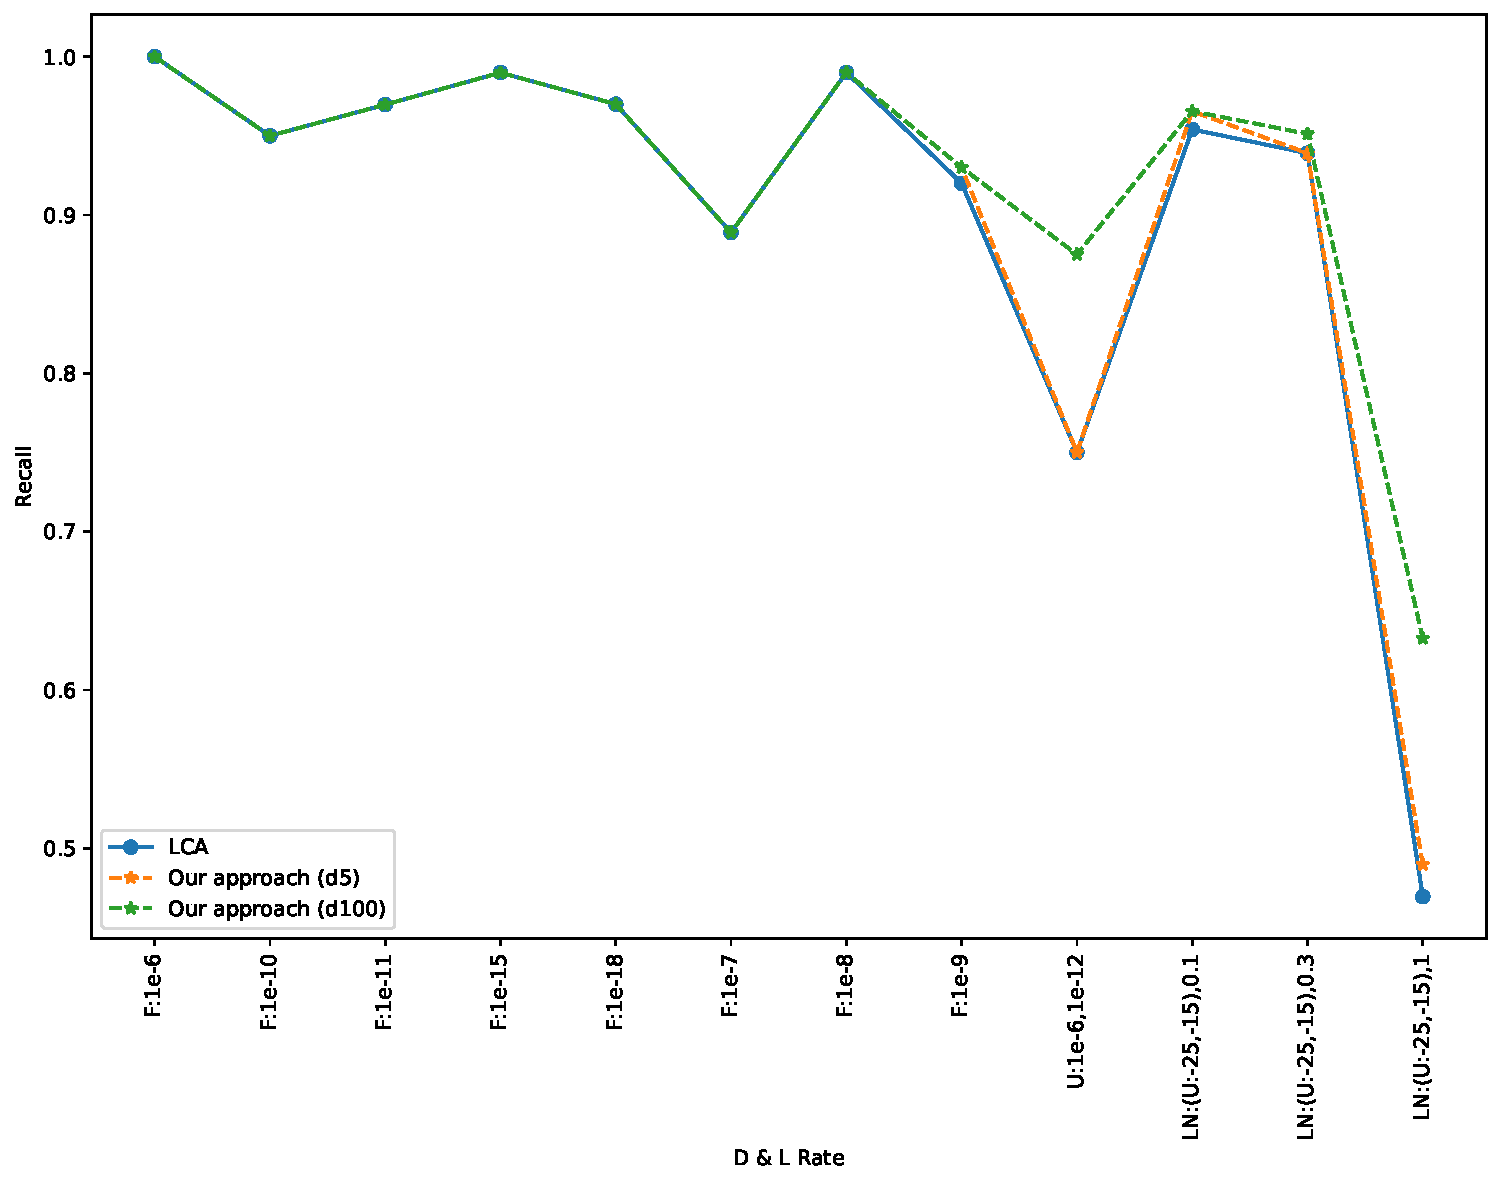
\includegraphics[width=\textwidth]{figs/recall-NNI-K1-WGD-t20-t80-Avg.pdf}
        \caption{Recall of WGDs for simulations with 1 WGD under NNI when k=1, averaged over 100 runs.}
        \label{fig:recall-NNI-k1-wgd}
    \end{subfigure}
    \hfill
    \begin{subfigure}[b]{0.31\textwidth}
        \centering
        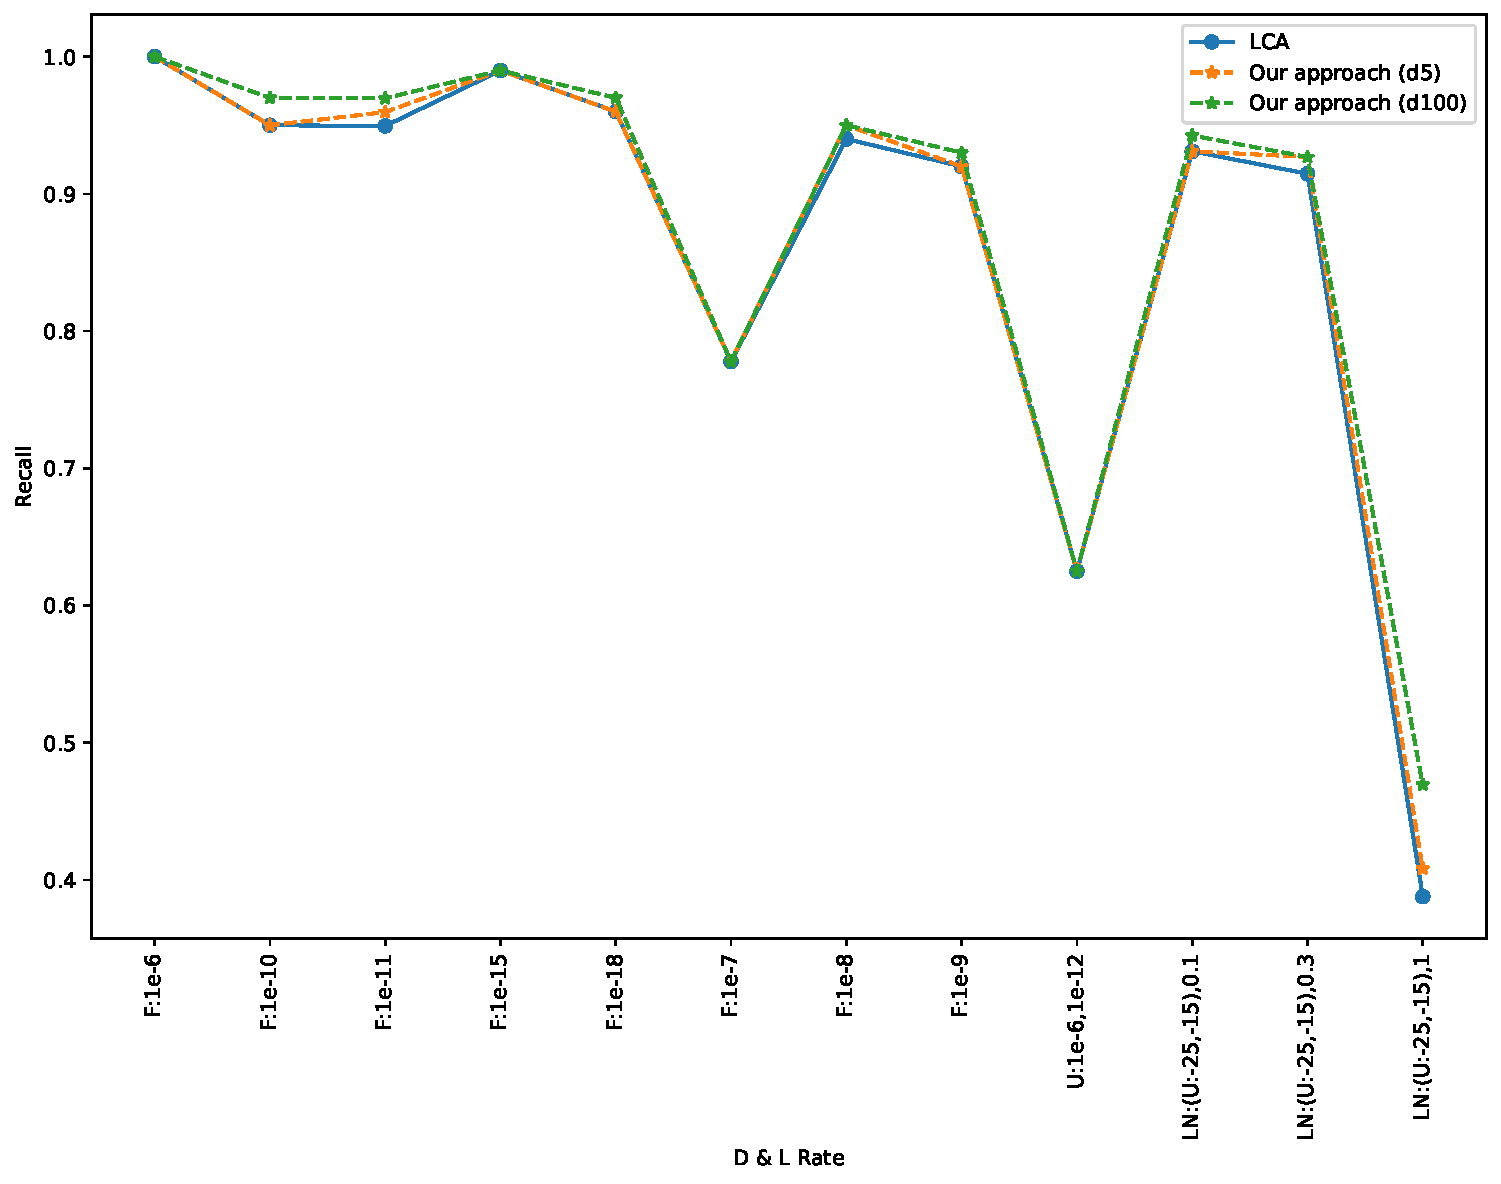
\includegraphics[width=\textwidth]{figs/recall-NNI-K5-WGD-t20-t80-Avg.pdf}
        \caption{Recall of WGDs for simulations with 1 WGD under NNI when k=5, averaged over 100 runs.}
        \label{fig:recall-NNI-k5-wgd}
    \end{subfigure}
    \hfill
    \begin{subfigure}[b]{0.31\textwidth}
        \centering
        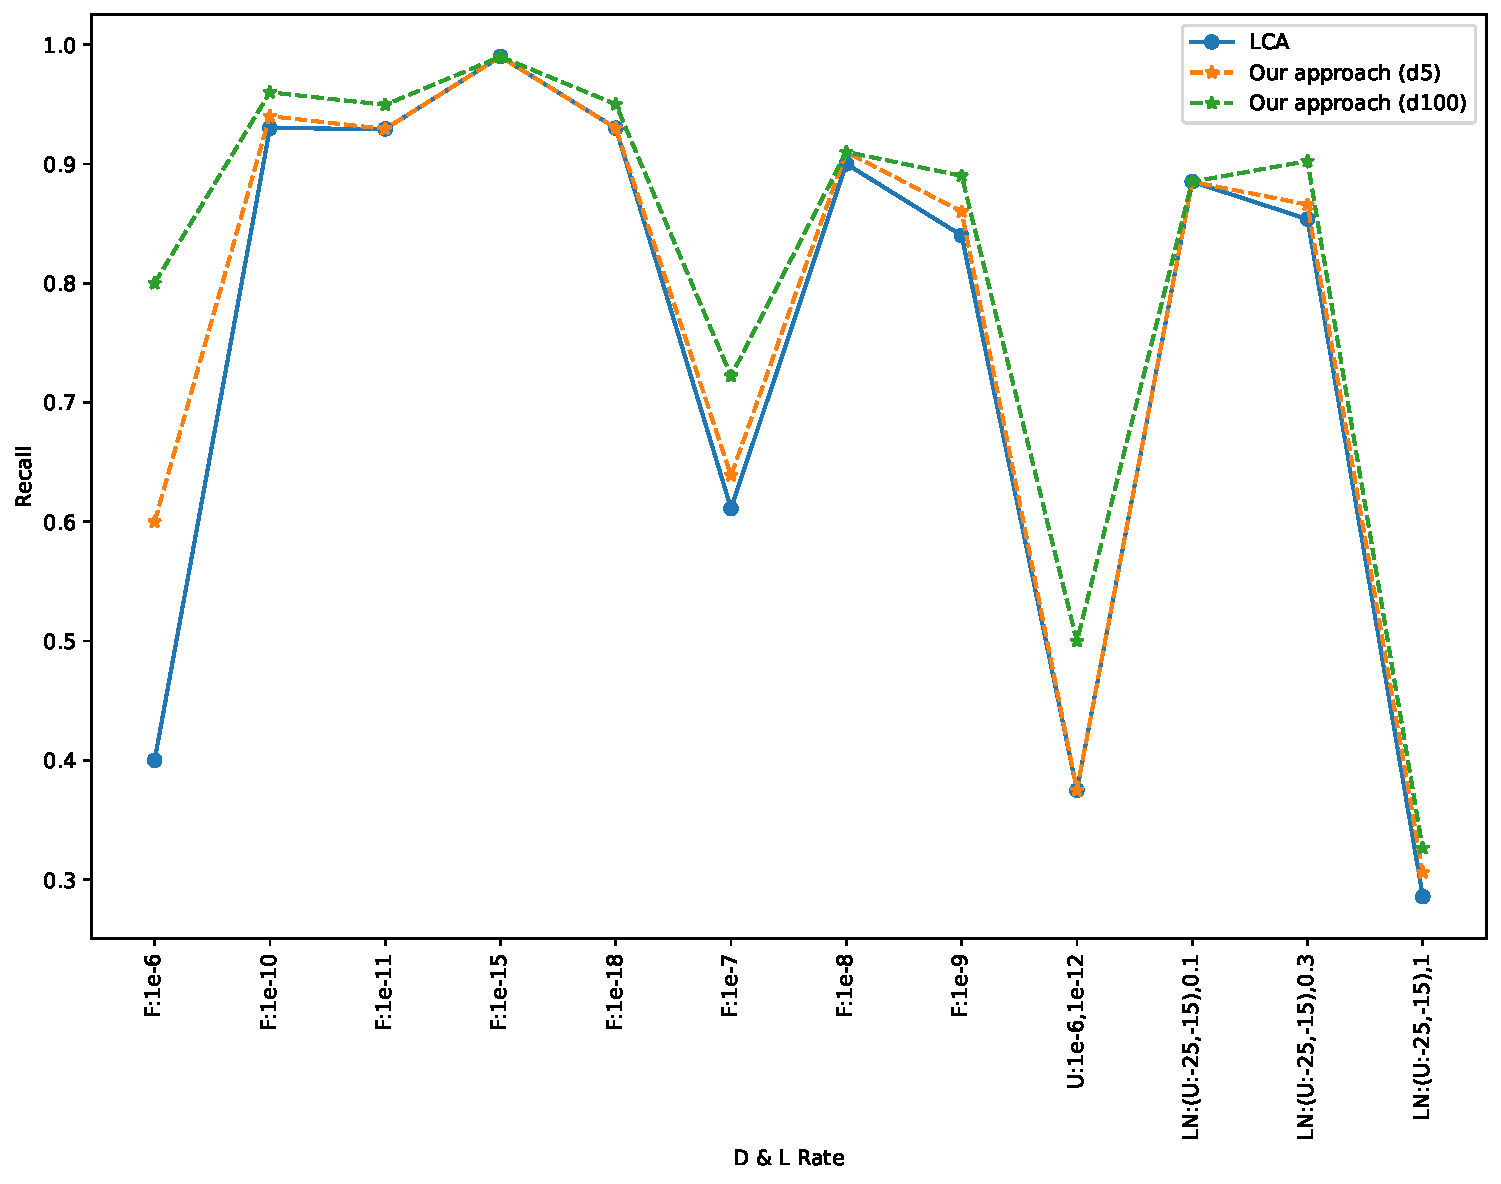
\includegraphics[width=\textwidth]{figs/recall-NNI-K15-WGD-t20-t80-Avg.pdf}
        \caption{Recall of WGDs for simulations with 1 WGD under NNI when k=15, averaged over 100 runs.}
        \label{fig:recall-NNI-k15-wgd}
    \end{subfigure}
    
    \vspace{1em} % Adds space between the two rows

    % Second row of three subplots
    \begin{subfigure}[b]{0.31\textwidth}
        \centering
        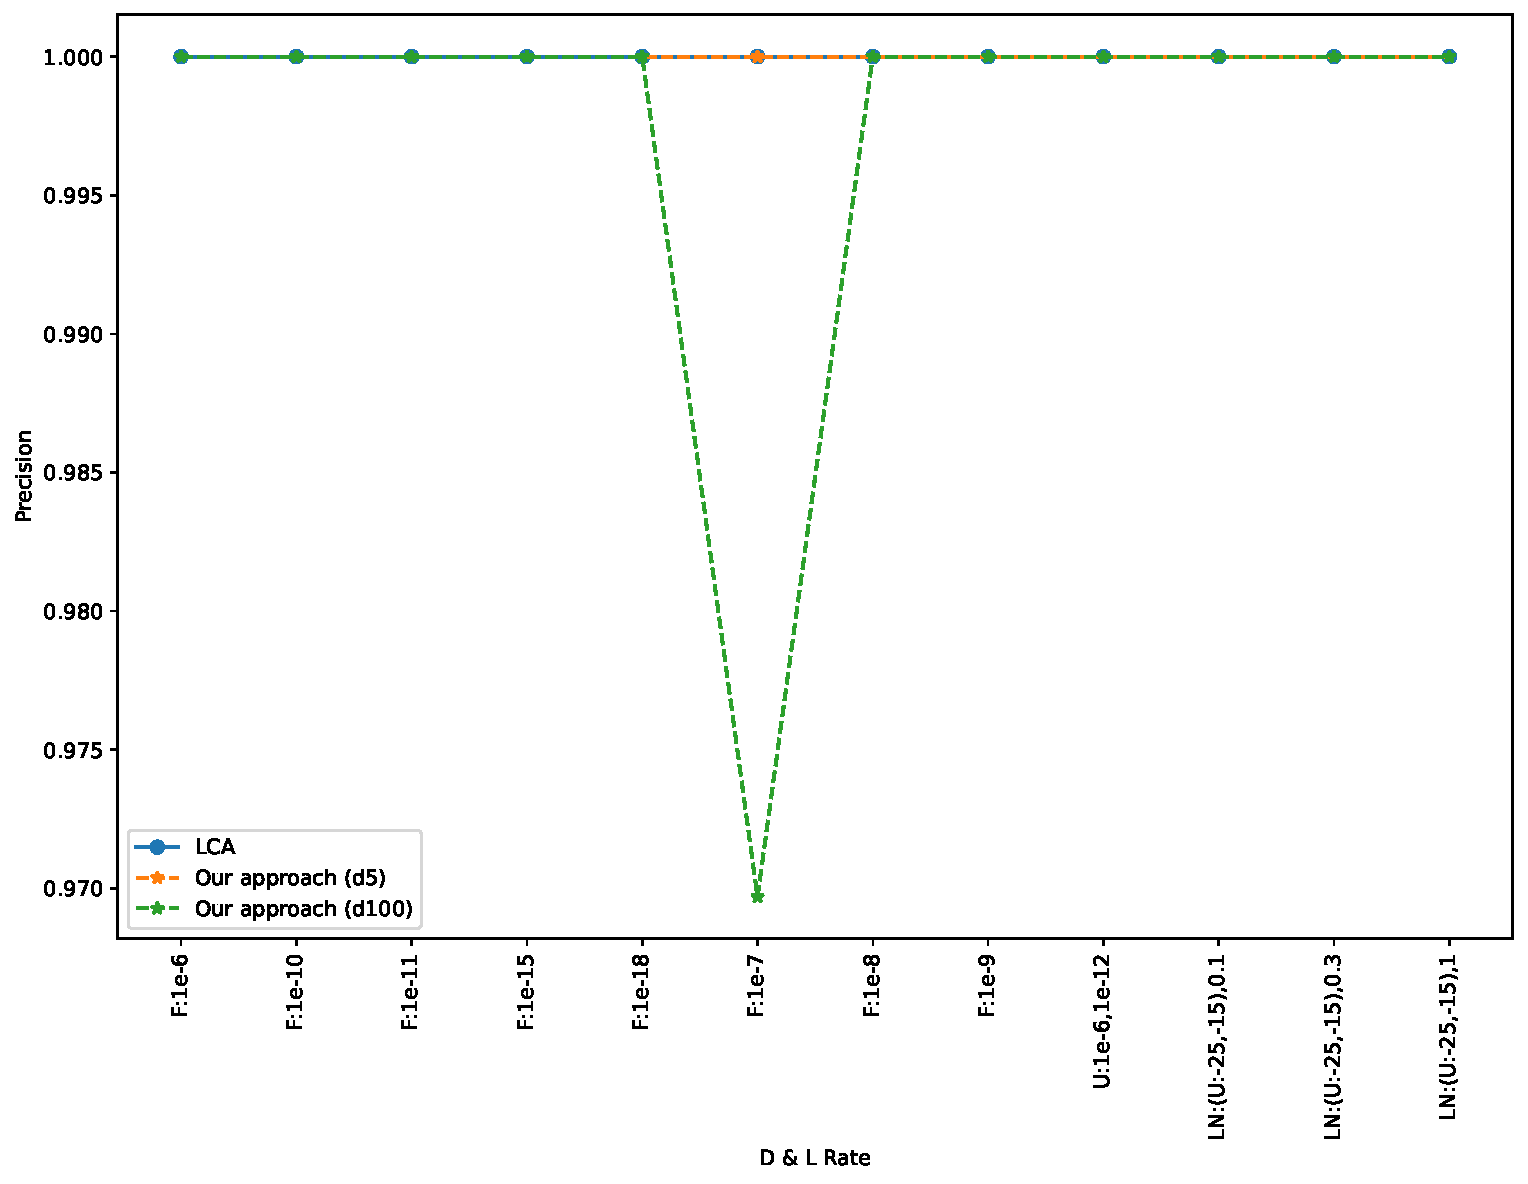
\includegraphics[width=\textwidth]{figs/precision-NNI-K1-WGD-t20-t80-Avg.pdf}
        \caption{Precision of WGDs for simulations with 1 WGD under NNI when k=1, averaged over 100 runs.}
        \label{fig:precision-NNI-k1-wgd}
    \end{subfigure}
    \hfill
    \begin{subfigure}[b]{0.31\textwidth}
        \centering
        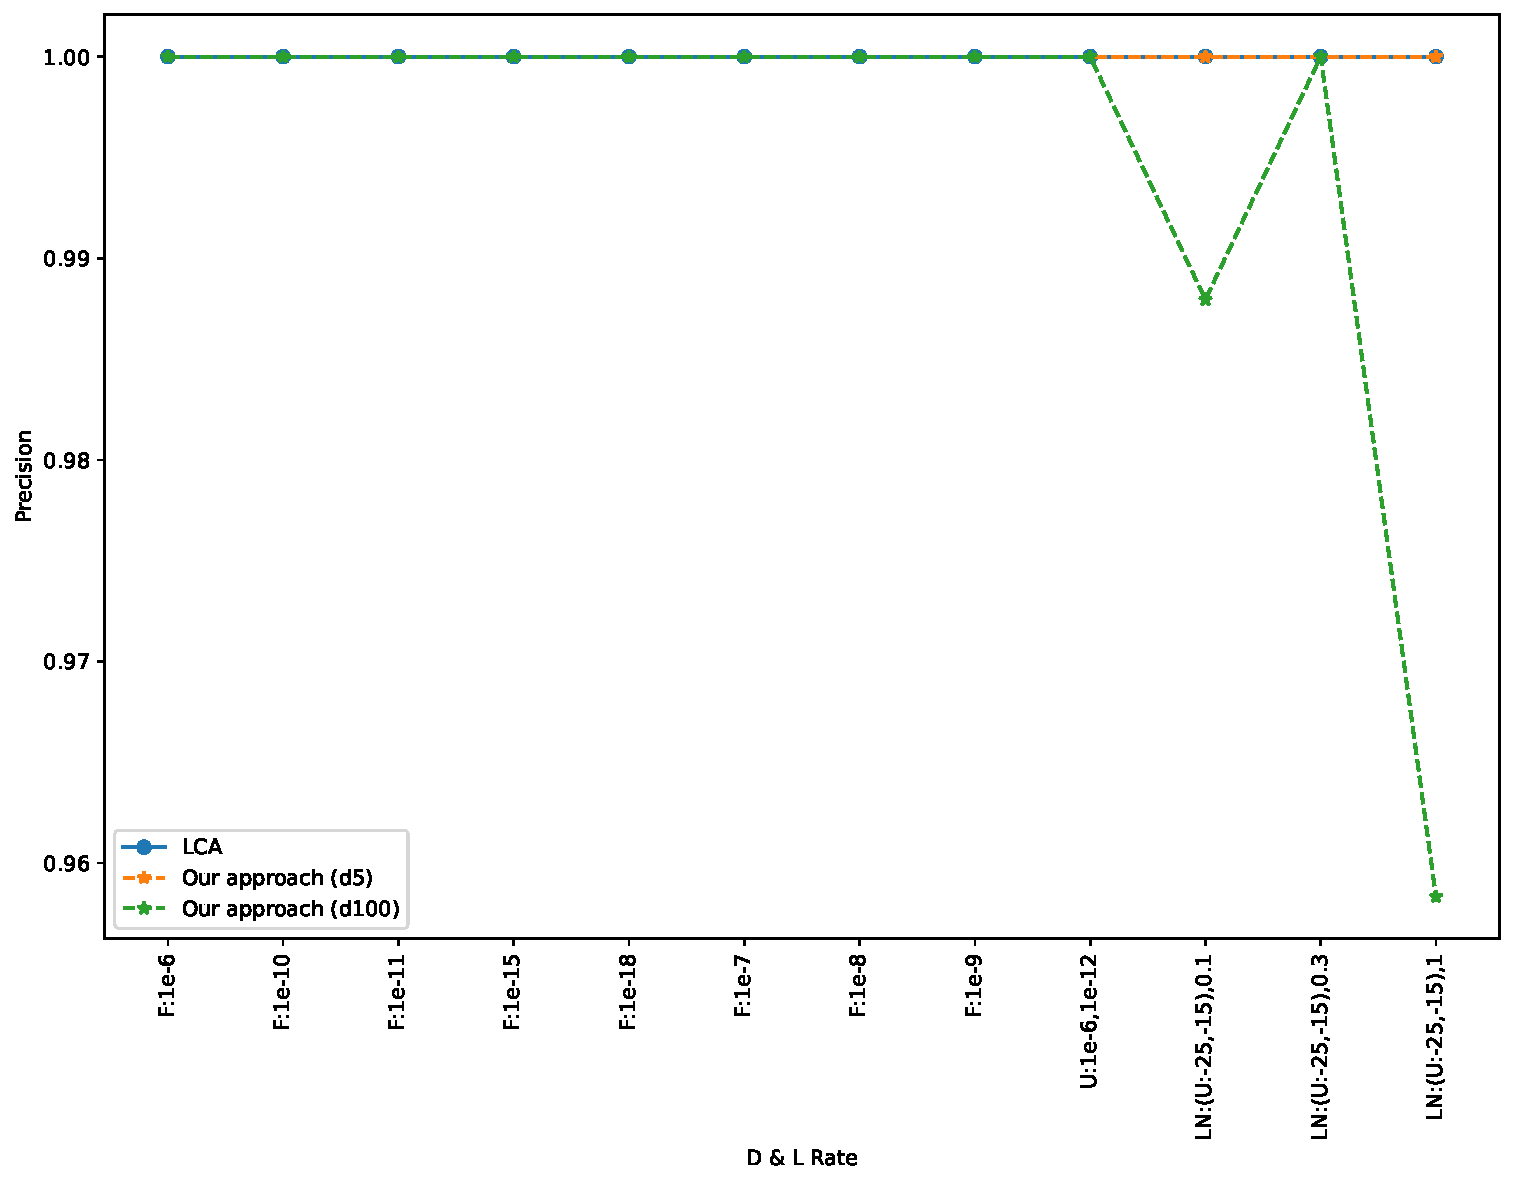
\includegraphics[width=\textwidth]{figs/precision-NNI-K5-WGD-t20-t80-Avg.pdf}
        \caption{Precision of WGDs for simulations with 1 WGD under NNI when k=5, averaged over 100 runs.}
        \label{fig:precision-NNI-k5-wgd}
    \end{subfigure}
    \hfill
    \begin{subfigure}[b]{0.31\textwidth}
        \centering
        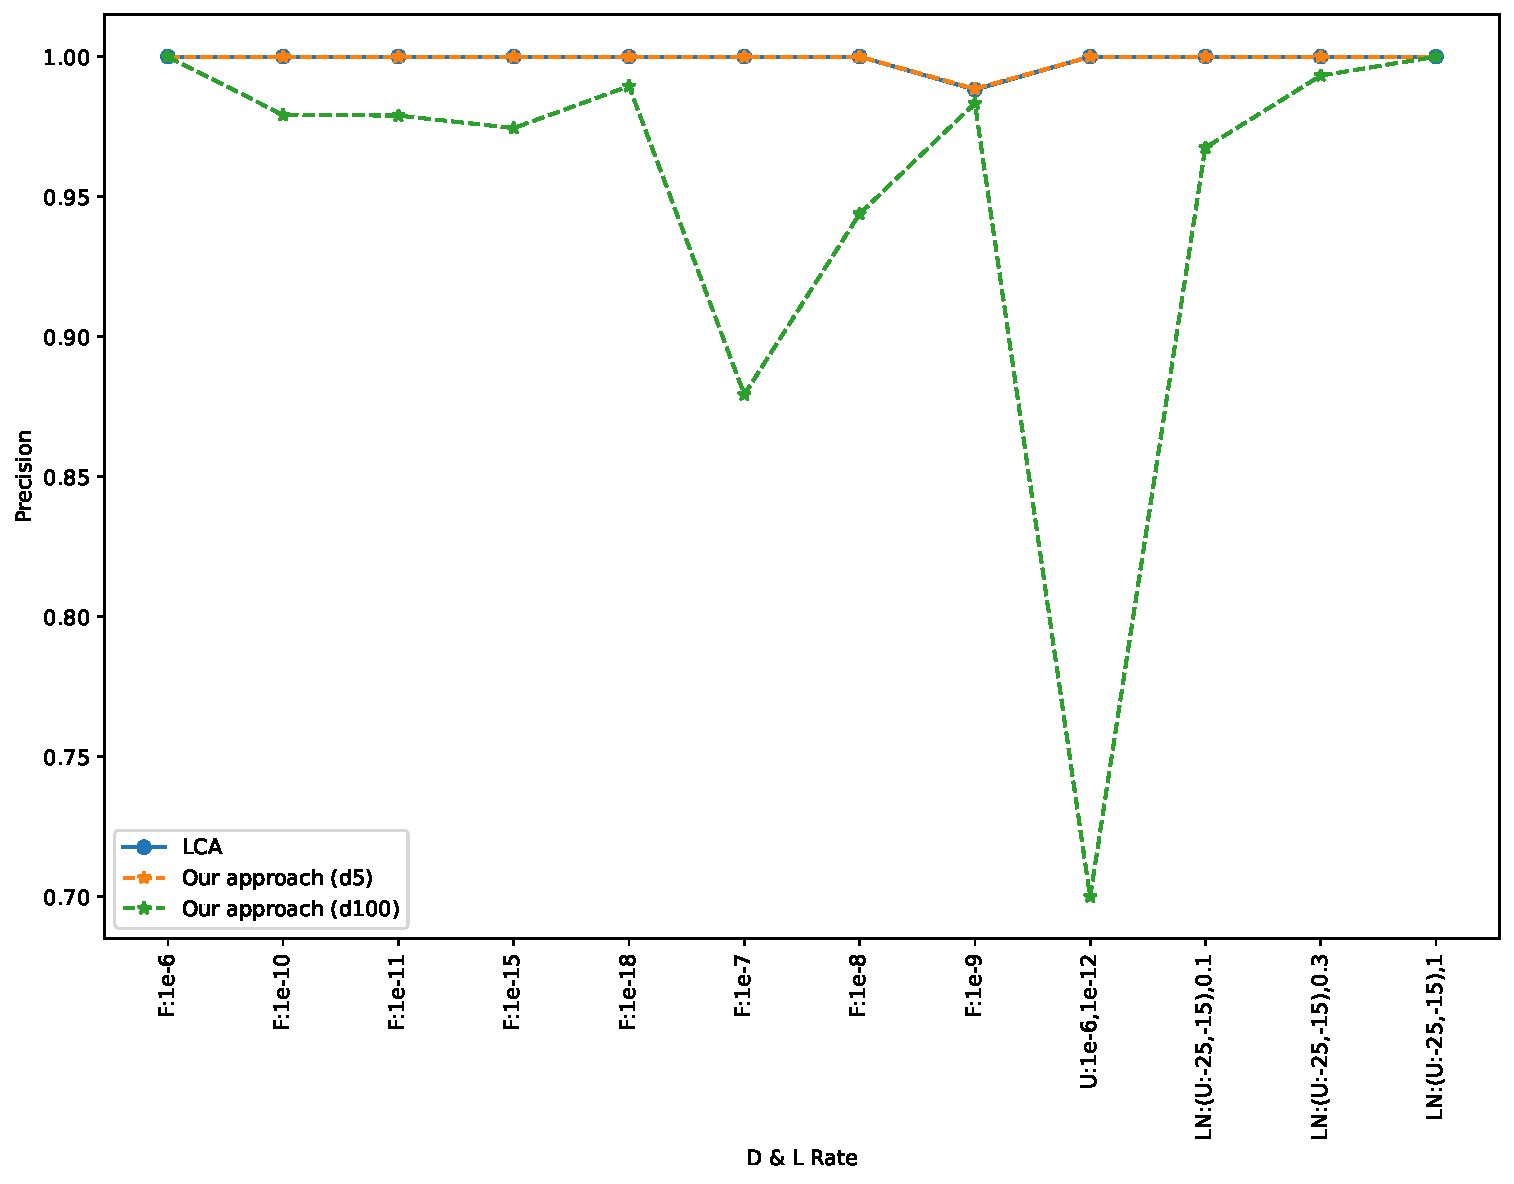
\includegraphics[width=\textwidth]{figs/precision-NNI-K15-WGD-t20-t80-Avg.pdf}
        \caption{Precision of WGDs for simulations with 1 WGD under NNI when k=15, averaged over 100 runs.}
        \label{fig:precision-NNI-k15-wgd}
    \end{subfigure}
    
    \caption{
        Comparison of Recall and Precision metrics for predicting Whole Genome Duplications (WGDs) in simulations with 1 WGD under Nearest Neighbor Interchanges (NNI) events. The parameter $k$ represents the number of NNIs applied to each gene tree. The simulations span varying duplication and loss rates and are averaged over 100 runs. Subfigures (a), (b), and (c) show Recall metrics for $k=1$, $k=5$, and $k=15$ NNIs, respectively. Subfigures (d), (e), and (f) present the corresponding Precision metrics under the same conditions.
    }
    \label{fig:recall-precision-wgd-NNI}
\end{figure}


\begin{figure}[h!]
    \centering
    % First row of three subplots
    \begin{subfigure}[b]{0.31\textwidth}
        \centering
        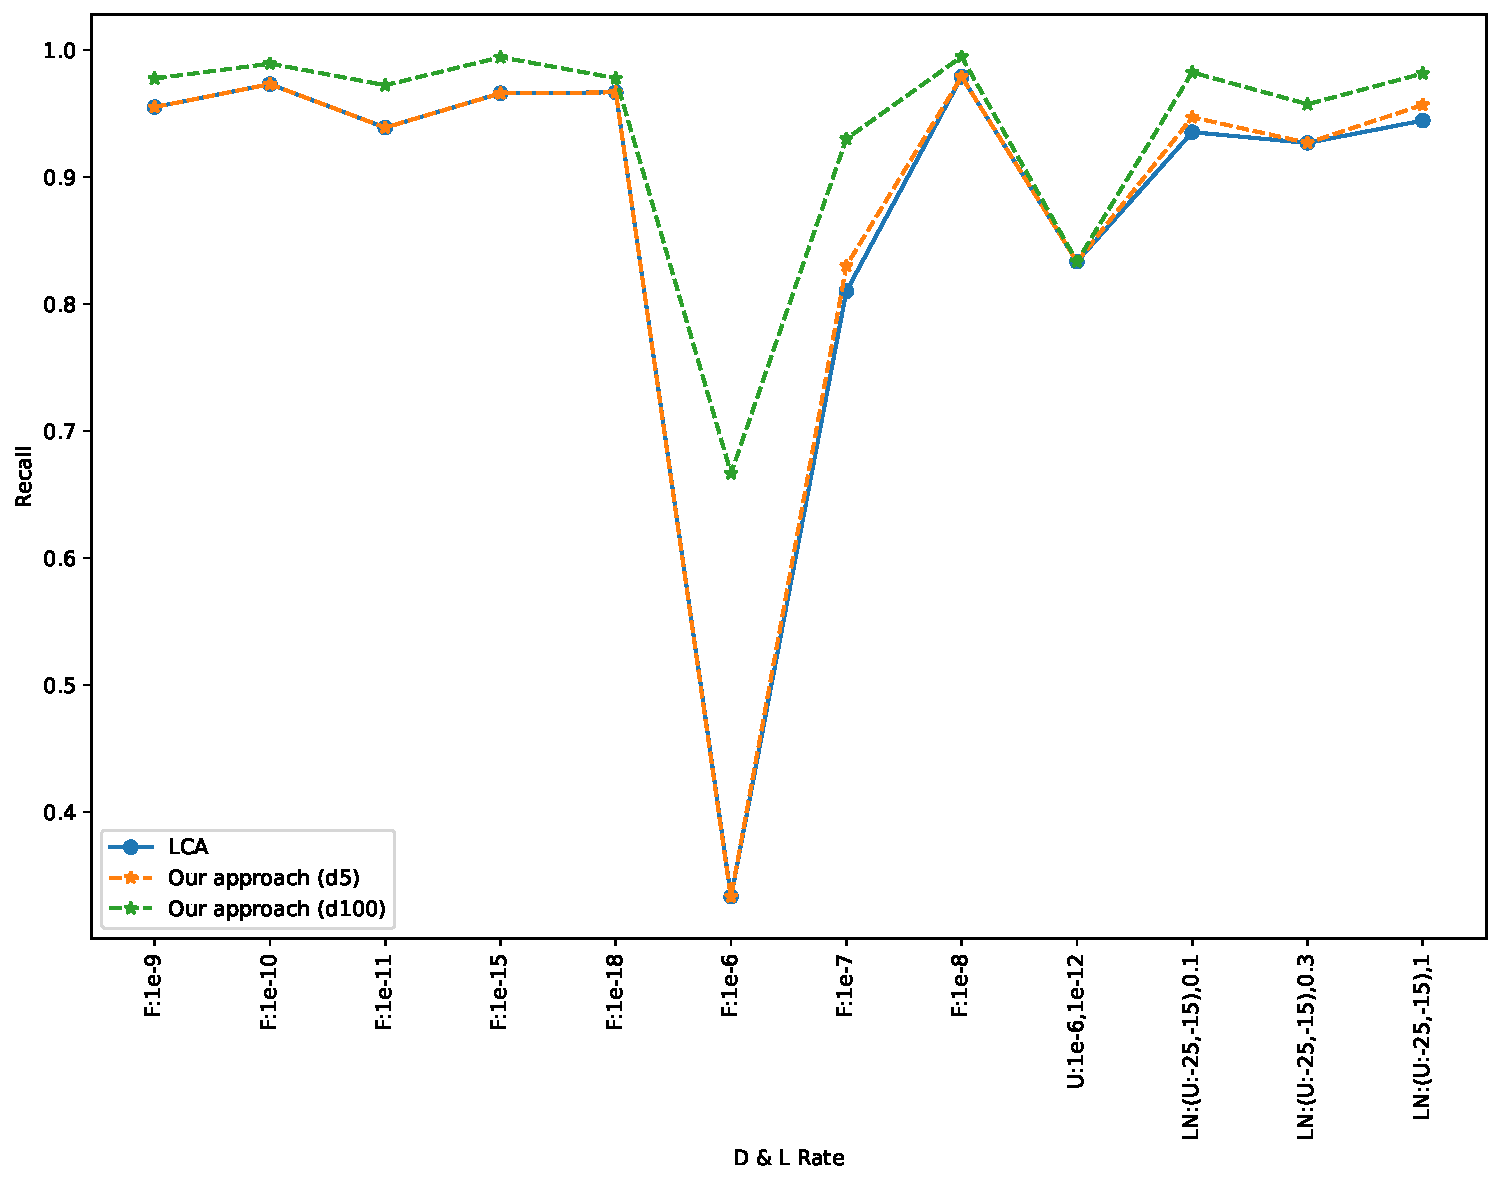
\includegraphics[width=\textwidth]{figs/recall-2W-NNI-K1-WGD-t20-t80-Avg.pdf}
        \caption{Recall of WGDs for simulations with 2 WGD under NNI when k=1, averaged over 100 runs.}
        \label{fig:recall-NNI-k1-2wgd}
    \end{subfigure}
    \hfill
    \begin{subfigure}[b]{0.31\textwidth}
        \centering
        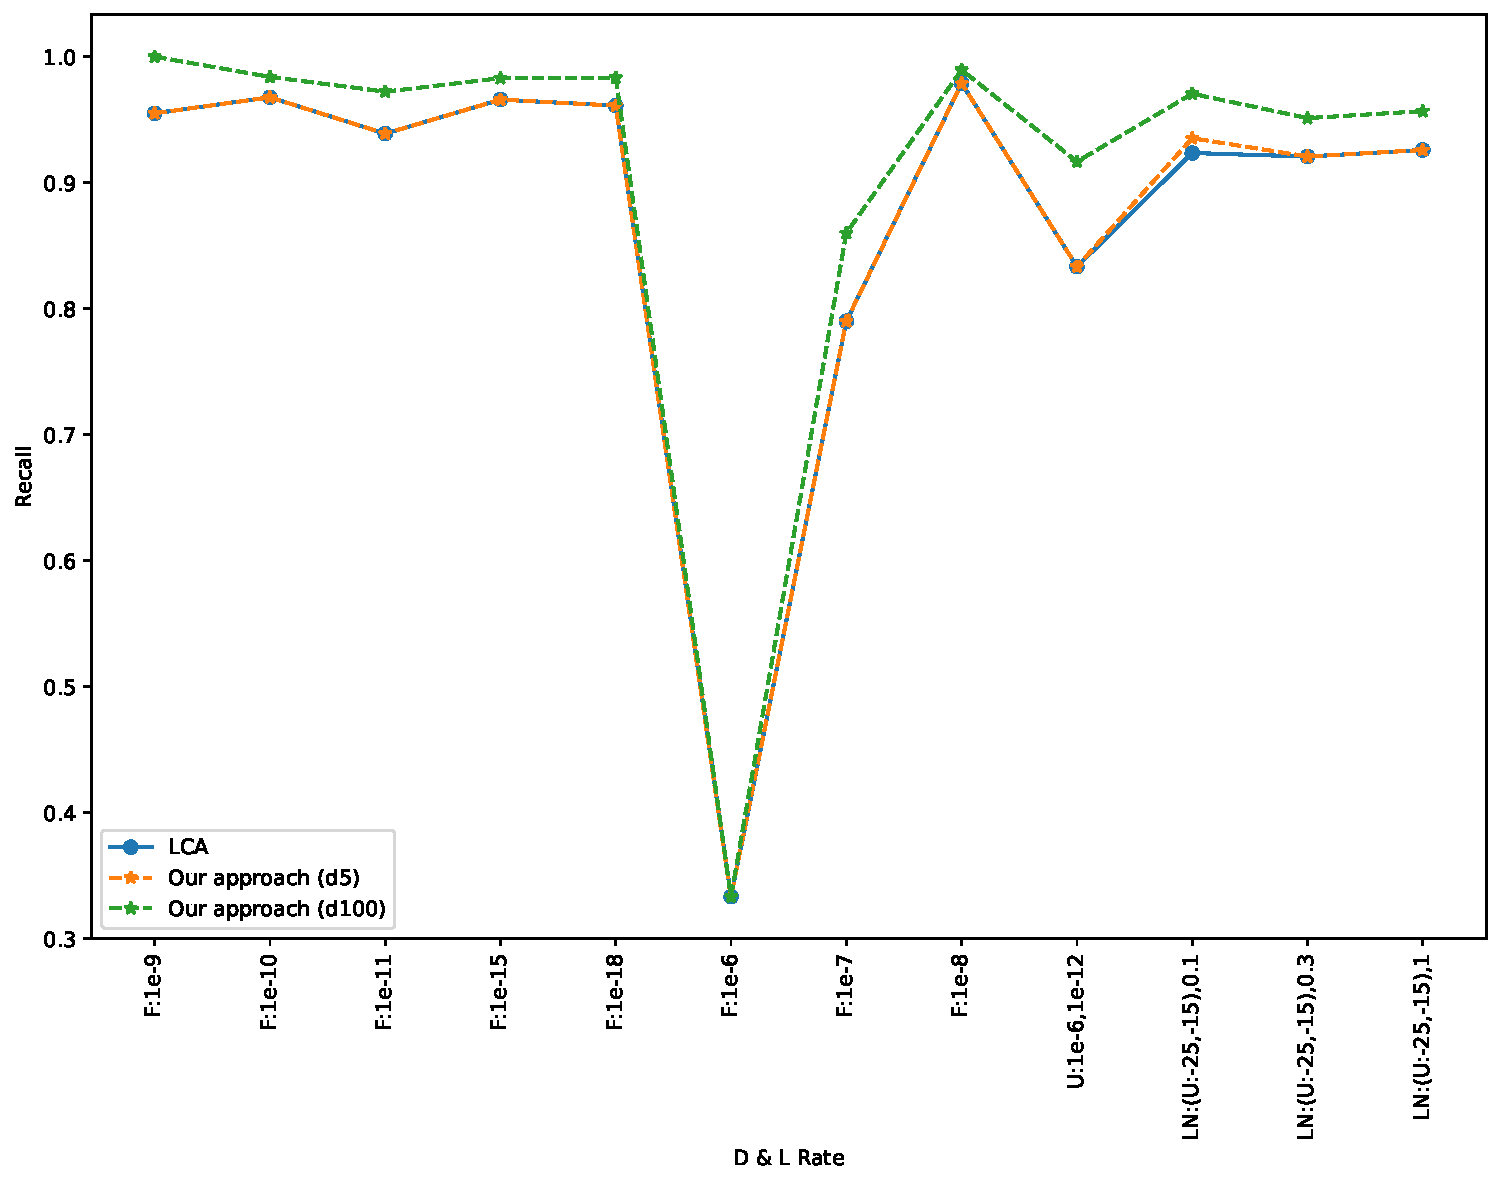
\includegraphics[width=\textwidth]{figs/recall-2W-NNI-K5-WGD-t20-t80-Avg.pdf}
        \caption{Recall of WGDs for simulations with 2 WGD under NNI when k=5, averaged over 100 runs.}
        \label{fig:recall-NNI-k5-2wgd}
    \end{subfigure}
    \hfill
    \begin{subfigure}[b]{0.31\textwidth}
        \centering
        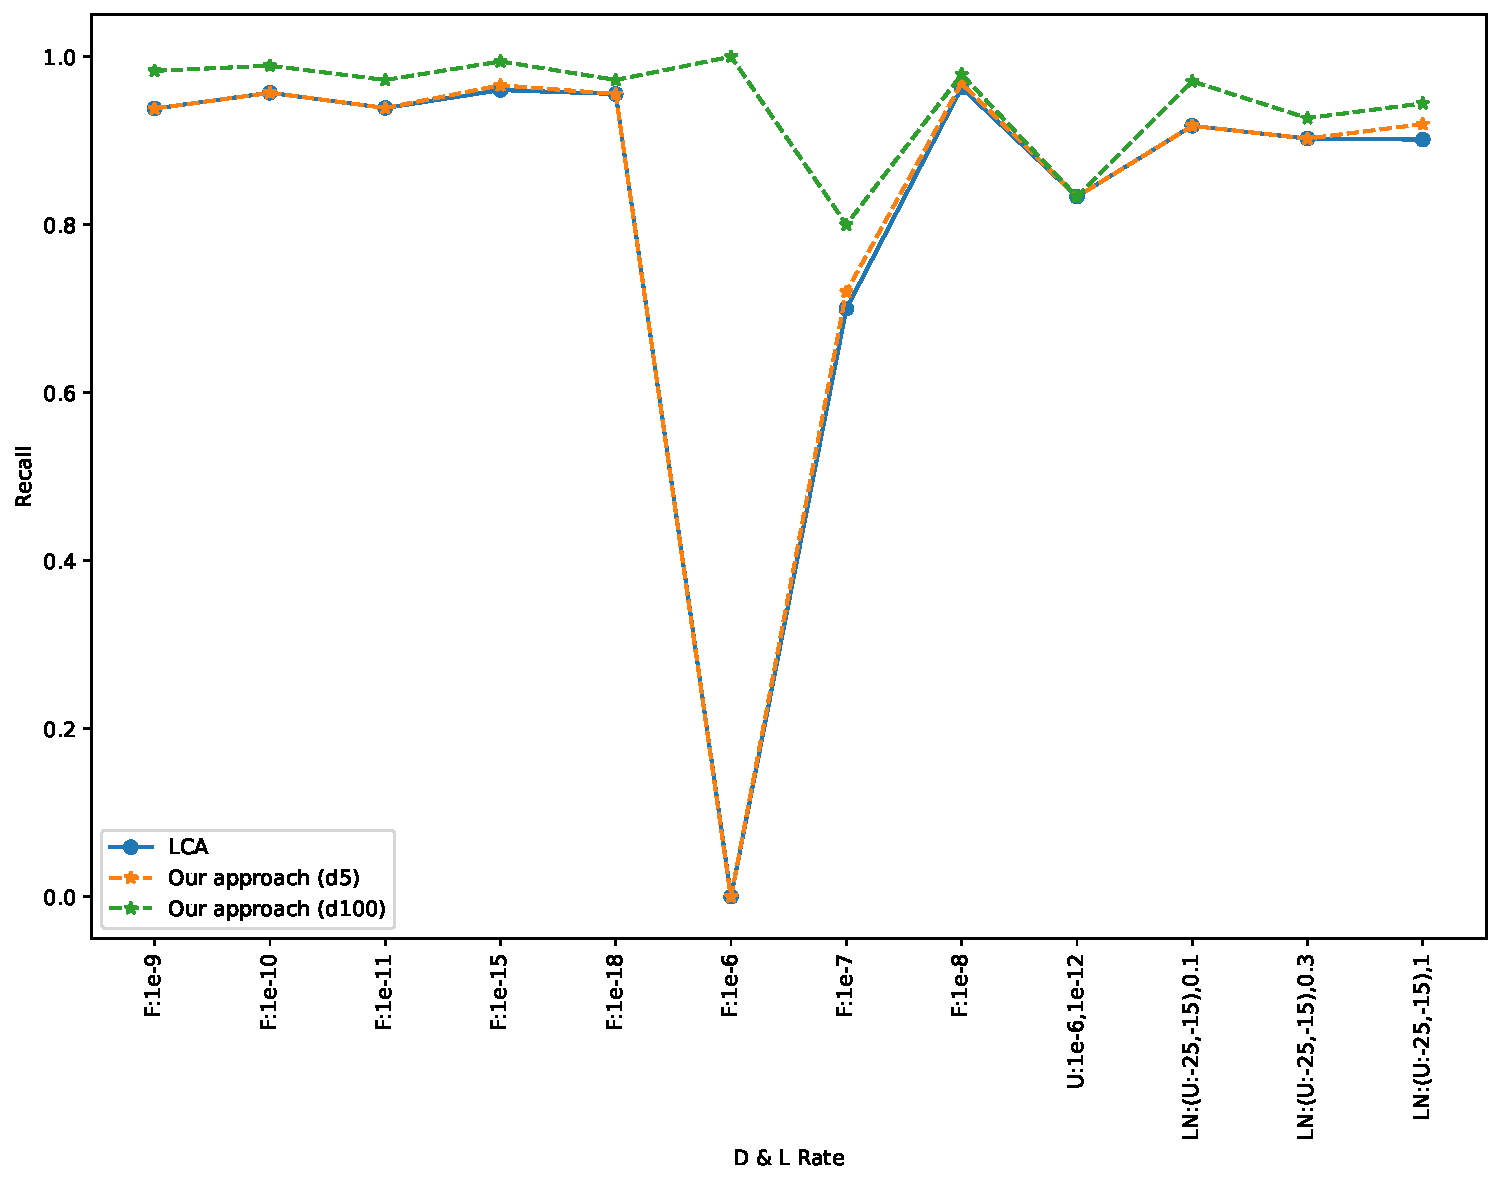
\includegraphics[width=\textwidth]{figs/recall-2W-NNI-K15-WGD-t20-t80-Avg.pdf}
        \caption{Recall of WGDs for simulations with 2 WGD under NNI when k=15, averaged over 100 runs.}
        \label{fig:recall-NNI-k15-2wgd}
    \end{subfigure}
    
    \vspace{1em} % Adds space between the two rows

    % Second row of three subplots
    \begin{subfigure}[b]{0.31\textwidth}
        \centering
        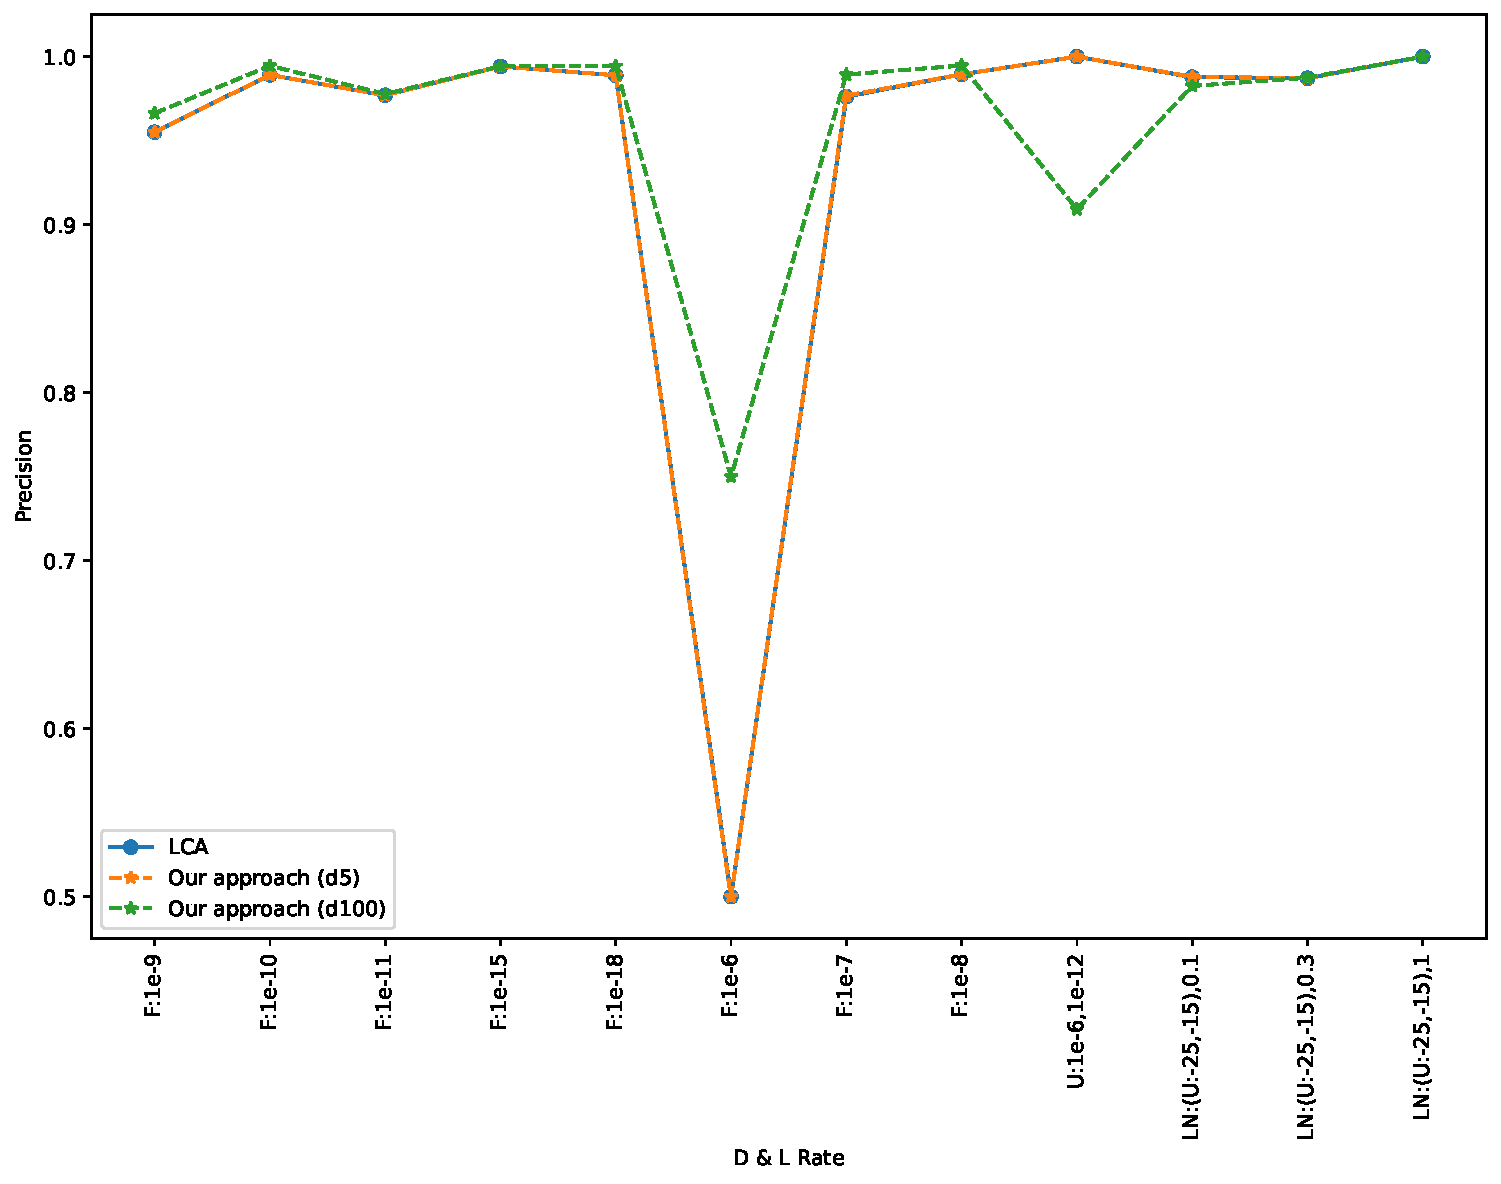
\includegraphics[width=\textwidth]{figs/precision-2W-NNI-K1-WGD-t20-t80-Avg.pdf}
        \caption{Precision of WGDs for simulations with 2 WGD under NNI when k=1, averaged over 100 runs.}
        \label{fig:precision-NNI-k1-2wgd}
    \end{subfigure}
    \hfill
    \begin{subfigure}[b]{0.31\textwidth}
        \centering
        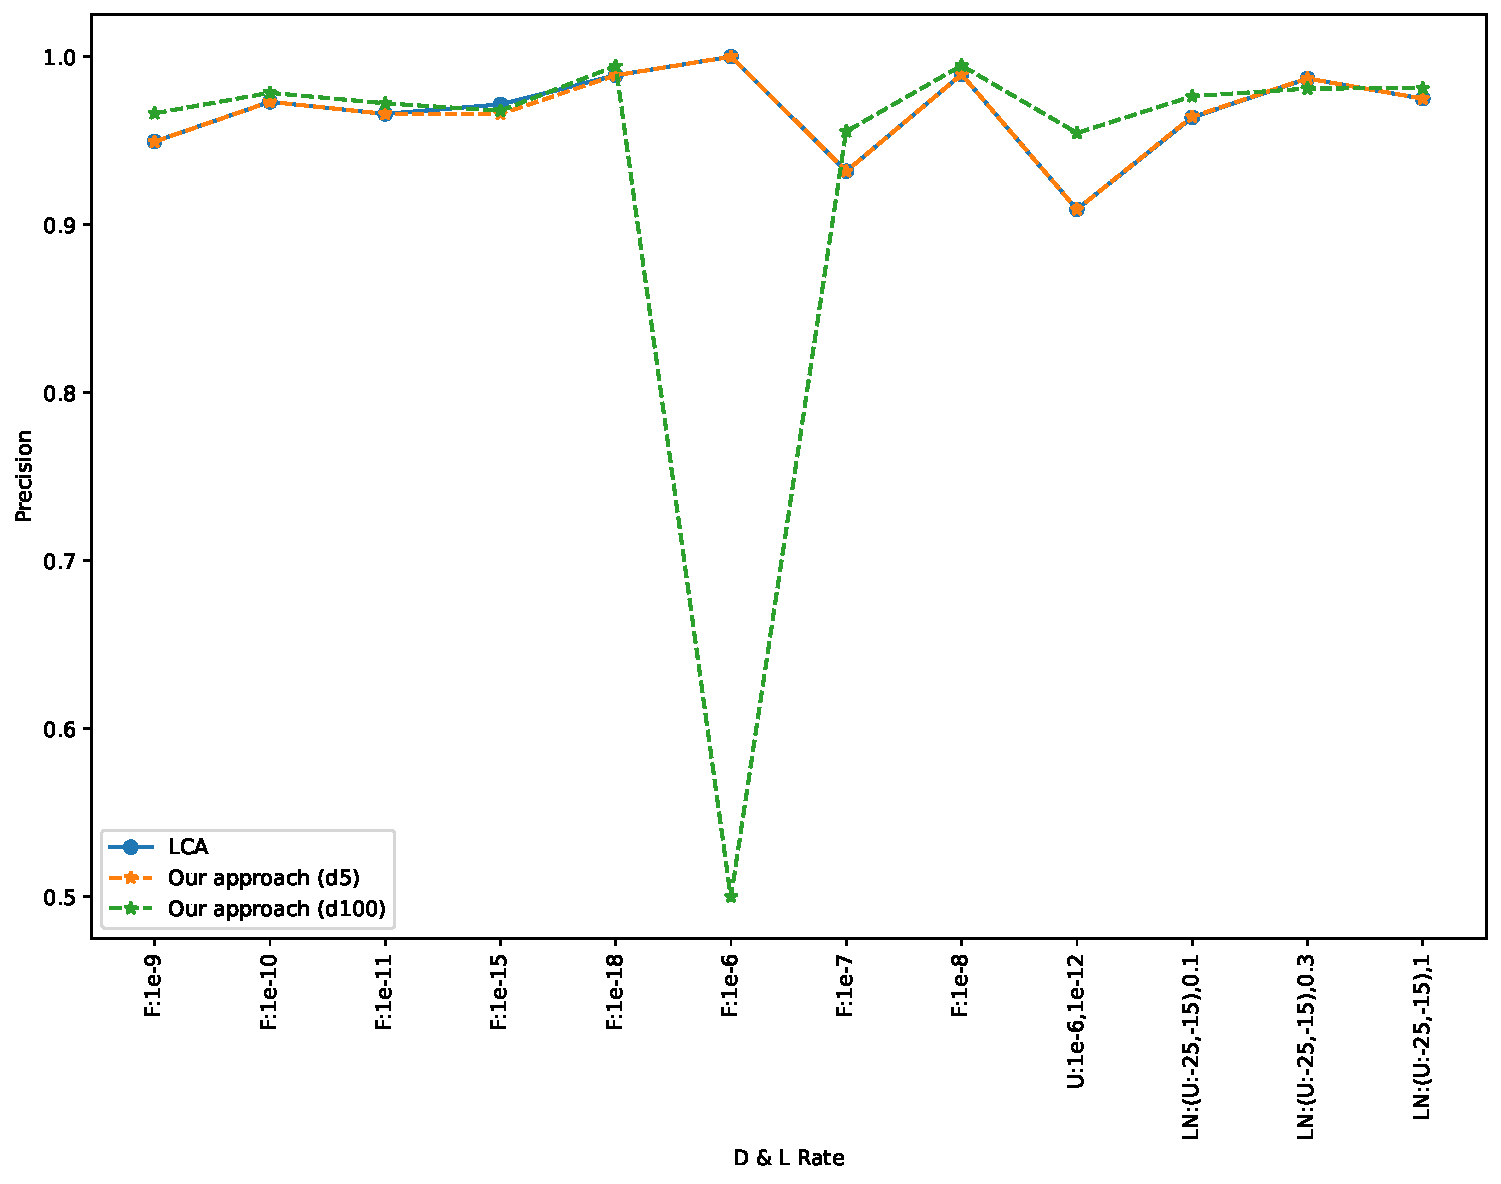
\includegraphics[width=\textwidth]{figs/precision-2W-NNI-K5-WGD-t20-t80-Avg.pdf}
        \caption{Precision of WGDs for simulations with 2 WGD under NNI when k=5, averaged over 100 runs.}
        \label{fig:precision-NNI-k5-2wgd}
    \end{subfigure}
    \hfill
    \begin{subfigure}[b]{0.31\textwidth}
        \centering
        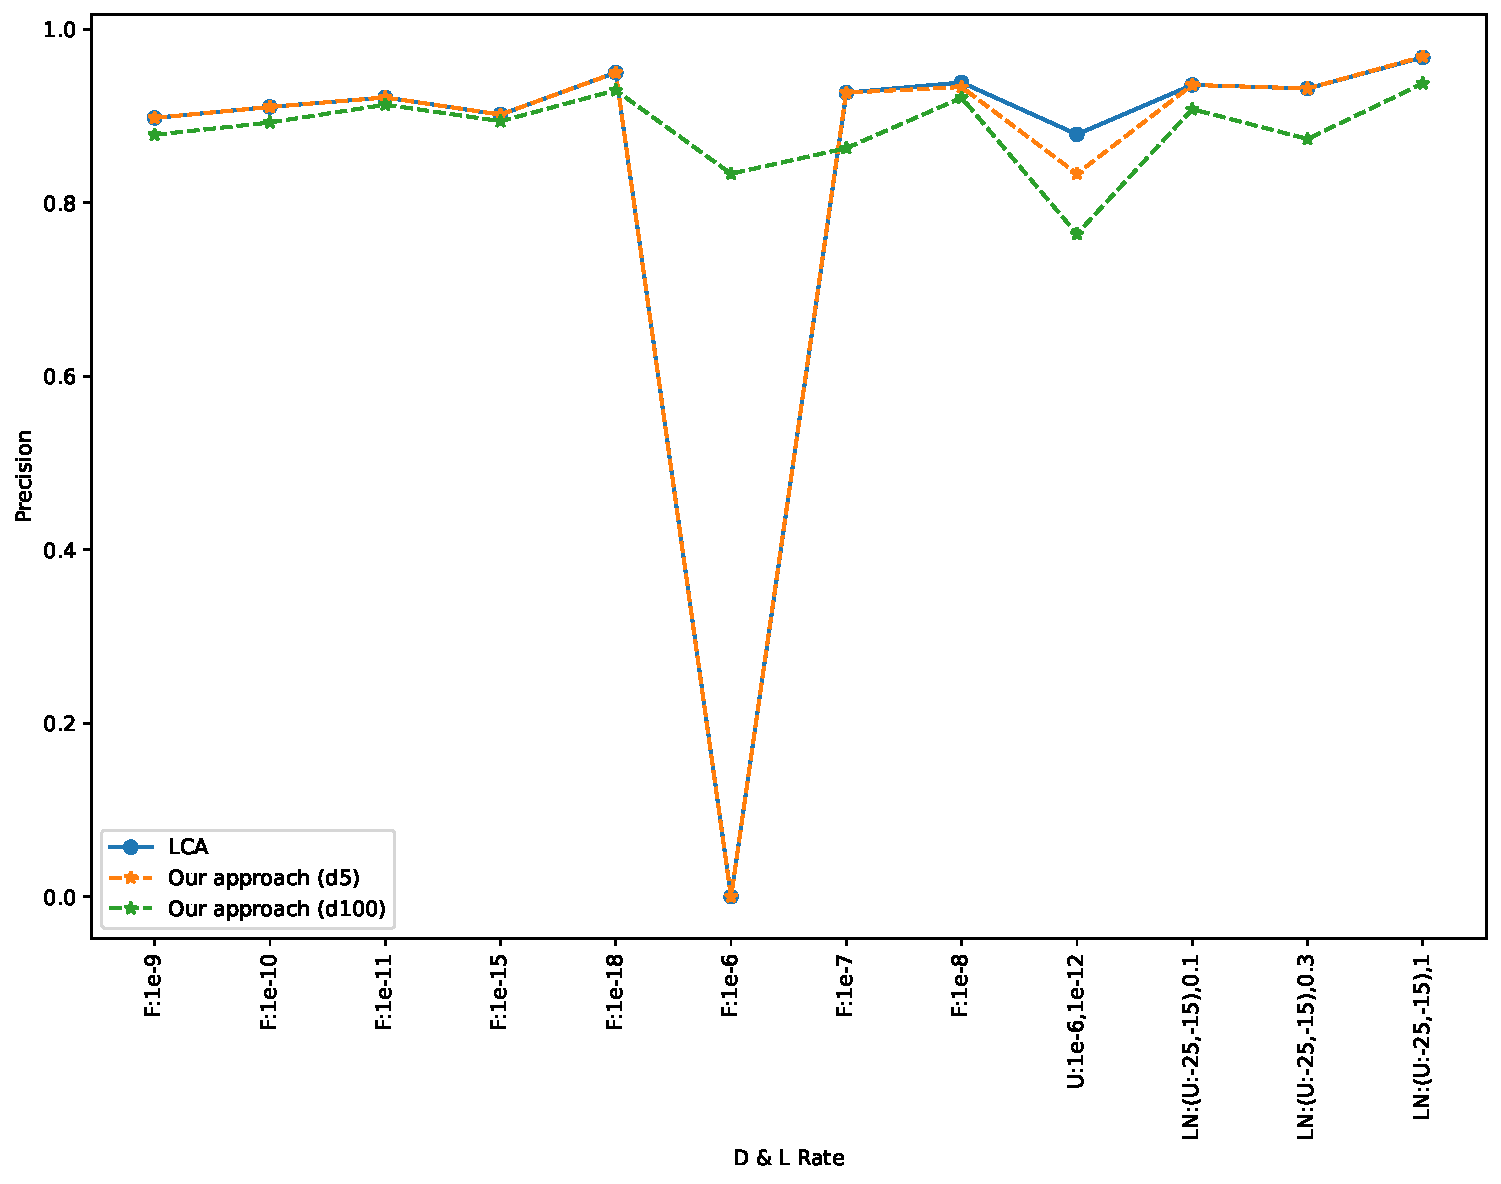
\includegraphics[width=\textwidth]{figs/precision-2W-NNI-K15-WGD-t20-t80-Avg.pdf}
        \caption{Precision of WGDs for simulations with 2 WGD under NNI when k=15, averaged over 100 runs.}
        \label{fig:precision-NNI-k15-2wgd}
    \end{subfigure}
    
    \caption{
        Comparison of Recall and Precision metrics for predicting Whole Genome Duplications (WGDs) in simulations with 2 WGD under Nearest Neighbor Interchanges (NNI) events. The parameter $k$ represents the number of NNIs applied to each gene tree. The simulations span varying duplication and loss rates and are averaged over 100 runs. Subfigures (a), (b), and (c) show Recall metrics for $k=1$, $k=5$, and $k=15$ NNIs, respectively. Subfigures (d), (e), and (f) present the corresponding Precision metrics under the same conditions.
    }
    \label{fig:recall-precision-2wgd-NNI}
\end{figure}

\newpage






\section{Acknowledgments}
This work was supported by French Agence Nationale de la Recherche through the CoCoAlSeq project (ANR-19-CE45-0012). This is the contribution ISEM 2024-XXX of the Institut des Sciences de l’Evolution de Montpellier.


\bibliographystyle{plain}
\bibliography{ref}

\end{document}

